% Options for packages loaded elsewhere
\PassOptionsToPackage{unicode}{hyperref}
\PassOptionsToPackage{hyphens}{url}
%
\documentclass[
]{book}
\usepackage{amsmath,amssymb}
\usepackage{iftex}
\ifPDFTeX
  \usepackage[T1]{fontenc}
  \usepackage[utf8]{inputenc}
  \usepackage{textcomp} % provide euro and other symbols
\else % if luatex or xetex
  \usepackage{unicode-math} % this also loads fontspec
  \defaultfontfeatures{Scale=MatchLowercase}
  \defaultfontfeatures[\rmfamily]{Ligatures=TeX,Scale=1}
\fi
\usepackage{lmodern}
\ifPDFTeX\else
  % xetex/luatex font selection
\fi
% Use upquote if available, for straight quotes in verbatim environments
\IfFileExists{upquote.sty}{\usepackage{upquote}}{}
\IfFileExists{microtype.sty}{% use microtype if available
  \usepackage[]{microtype}
  \UseMicrotypeSet[protrusion]{basicmath} % disable protrusion for tt fonts
}{}
\makeatletter
\@ifundefined{KOMAClassName}{% if non-KOMA class
  \IfFileExists{parskip.sty}{%
    \usepackage{parskip}
  }{% else
    \setlength{\parindent}{0pt}
    \setlength{\parskip}{6pt plus 2pt minus 1pt}}
}{% if KOMA class
  \KOMAoptions{parskip=half}}
\makeatother
\usepackage{xcolor}
\usepackage{longtable,booktabs,array}
\usepackage{calc} % for calculating minipage widths
% Correct order of tables after \paragraph or \subparagraph
\usepackage{etoolbox}
\makeatletter
\patchcmd\longtable{\par}{\if@noskipsec\mbox{}\fi\par}{}{}
\makeatother
% Allow footnotes in longtable head/foot
\IfFileExists{footnotehyper.sty}{\usepackage{footnotehyper}}{\usepackage{footnote}}
\makesavenoteenv{longtable}
\usepackage{graphicx}
\makeatletter
\def\maxwidth{\ifdim\Gin@nat@width>\linewidth\linewidth\else\Gin@nat@width\fi}
\def\maxheight{\ifdim\Gin@nat@height>\textheight\textheight\else\Gin@nat@height\fi}
\makeatother
% Scale images if necessary, so that they will not overflow the page
% margins by default, and it is still possible to overwrite the defaults
% using explicit options in \includegraphics[width, height, ...]{}
\setkeys{Gin}{width=\maxwidth,height=\maxheight,keepaspectratio}
% Set default figure placement to htbp
\makeatletter
\def\fps@figure{htbp}
\makeatother
\setlength{\emergencystretch}{3em} % prevent overfull lines
\providecommand{\tightlist}{%
  \setlength{\itemsep}{0pt}\setlength{\parskip}{0pt}}
\setcounter{secnumdepth}{5}
\usepackage{booktabs}
\usepackage{amsthm}
\makeatletter
\def\thm@space@setup{%
  \thm@preskip=8pt plus 2pt minus 4pt
  \thm@postskip=\thm@preskip
}
\makeatother
\ifLuaTeX
  \usepackage{selnolig}  % disable illegal ligatures
\fi
\usepackage[]{natbib}
\bibliographystyle{apalike}
\IfFileExists{bookmark.sty}{\usepackage{bookmark}}{\usepackage{hyperref}}
\IfFileExists{xurl.sty}{\usepackage{xurl}}{} % add URL line breaks if available
\urlstyle{same}
\hypersetup{
  pdftitle={MAT 121 E-Pack: Statistics I},
  pdfauthor={Cheng Peng},
  hidelinks,
  pdfcreator={LaTeX via pandoc}}

\title{MAT 121 E-Pack: Statistics I}
\author{Cheng Peng}
\date{West Chester University}

\begin{document}
\maketitle

{
\setcounter{tocdepth}{1}
\tableofcontents
}
\hypertarget{introduction}{%
\chapter{Introduction}\label{introduction}}

This \emph{E-Pack} is a self-contained homegrown Ebook that contains all topics covered in current MAT 121 at WCU.

All technical terms used in this Ebook are consistent with those used in the \emph{required} textbook. There several benefits of using this \emph{E-Pack}:

\begin{itemize}
\item
  All technical terms used in this eBook are consistent with those used in the \emph{required} textbook.
\item
  Three formats (PDF, HTML, and EPub) of the E-Pack are accessible from different devices.
\item
  In the HTML version, there are many animated graphics as well as decorative visual aids such as font size, colors, etc. to make some concepts more intuitive.
\item
  The supplement course website {[}\url{https://pengdsci.github.io/MAT121/}{]} has topic-wise online practice problems for most of the topics.
\item
  17 homegrown interactive statistics learning apps (ISLA) {[}\url{https://pengdsci.github.io/ISLA/}{]} covers all topics in this course. These apps can be used in two ways:

  \begin{itemize}
  \tightlist
  \item
    play around with the apps associated with each topic to enhance your understanding of the topics;
  \item
    use these apps as \textbf{solution generator} to check your work. Yes. They can generator answers to your questions! I used these apps generated answers to many examples
  \end{itemize}
\end{itemize}

\hypertarget{frequency-tables-and-charts}{%
\chapter{Frequency Tables and Charts}\label{frequency-tables-and-charts}}

\hypertarget{basic-statistical-terminologies}{%
\section{Basic Statistical Terminologies}\label{basic-statistical-terminologies}}

In this note, we introduce basic terminology of statistics and methods for summarizing a given data set.

\hypertarget{what-is-statistics}{%
\subsection{What is statistics?}\label{what-is-statistics}}

\begin{quote}
Statistics is the science of collecting, organizing, visualizing, analyzing, and interpreting data in order to make decision.
\end{quote}

\hypertarget{population-vs-sample}{%
\subsection{Population vs Sample}\label{population-vs-sample}}

\begin{itemize}
\item
  \textbf{Population}: The collection of \textbf{all} outcomes, responses, measurements, or counts that are of interest (the right group in the following figure).
\item
  \textbf{Sample}: A subset of the population (the left group in the following figure).
\end{itemize}

\begin{center}
\includegraphics[width=0.6\linewidth]{week01/popSample} \end{center}

\begin{itemize}
\item
  \textbf{Parameter}: the numeric characteristic of the population. For example, the average height of \textbf{all} students at WCU. Here \texttt{all\ WCU\ students} is a population.
\item
  \textbf{Statistic}: the numeric characteristic of the sample (i.e., a subset of the population). For example, the average height of \textbf{subset of} students at WCU. Here \texttt{the\ subset\ of\ WCU\ students} is a sample taken from the population of all WCU students.
\end{itemize}

\hypertarget{types-statistics-and-data}{%
\subsection{Types Statistics and Data}\label{types-statistics-and-data}}

\begin{itemize}
\item
  \textbf{Descriptive Statistics} involves organizing, summarizing, and displaying data. For example, we can use tables, charts, averages, etc. All topics in this note and next note will focus on descriptive statistics.
\item
  \textbf{Inferential Statistics} uses the sample data to make inferences about the underlying population. For example, all topics from week \#3 are inferential statistics.
\item
  \textbf{Data Types}: There different ways for classifying data in statistics. The following diagram given one of the simple bu widely used methods.
\end{itemize}

\begin{center}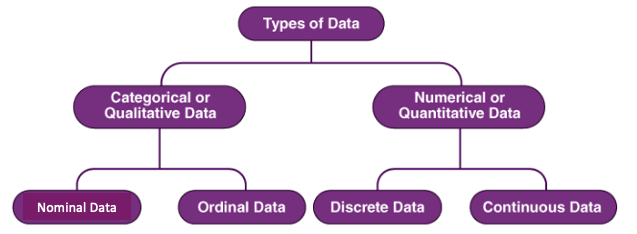
\includegraphics[width=0.7\linewidth]{week01/dataTypes} \end{center}

\begin{itemize}
\item
  \textbf{Data Types} examples

  \begin{itemize}
  \tightlist
  \item
    Nominal Data (also called unordered data): the place of birth, major, eye color, etc.
  \item
    Ordinal Data: Military Rank (private, corporal, etc.), Course Grade (A, B, C, D, F), etc.
  \item
    Discrete (a subset of which is ``counting''): Number of children in a family, Shoe Size, etc.
  \item
    Continuous: Weight, Height, temperature, income, GPA, etc.
  \end{itemize}
\end{itemize}

\hypertarget{summarizing-qualitative-data}{%
\section{Summarizing Qualitative Data}\label{summarizing-qualitative-data}}

For a given categorical data, we can use frequency tables and charts to summarize the distribution of the data. Note that the given data set could either be a population or a sample.

\hypertarget{frequency-tables}{%
\subsection{Frequency Tables}\label{frequency-tables}}

Since each distinct data value represents a category, the number of values in each category is the frequency of the category. \texttt{An\ ordinary\ frequency\ table} is a two-column table in which the left column lists the category labels and the right column lists the corresponding frequencies.

There are four types of frequency tables. The other three frequency tables are relative frequency table, cumulative frequency table, cumulative relative frequency table.

\texttt{a\ relative\ frequency\ =\ ordinary\ frequency\ /\ total}

\texttt{a\ cumulative\ frequeny\ table} is constructed based on the cumulatively combined categories. See the following example for more detail.

\textbf{Example 1}: In a class of 20 students, 3 students received a grade of ``A'', 6 students received a ``B'', 7 students received a ``C'', 3 students received a ``D'', and 1 student received an ``F''. These results are summarized, in a variety of ways, in the following table: (Note that for the ordered categorical variable ``Grade'' we also create the discrete quantitative variable ``Grade-point''.)

\textbf{Solution}: The raw data might be in the following form:

\begin{verbatim}
A,  C,  B,  F,  D,  B,  C,  B,  C,  C,  A,  D,  C,  B,  C,  B,  A,  C,  B,  D
\end{verbatim}

The resulting frequency tables is given by

\begin{center}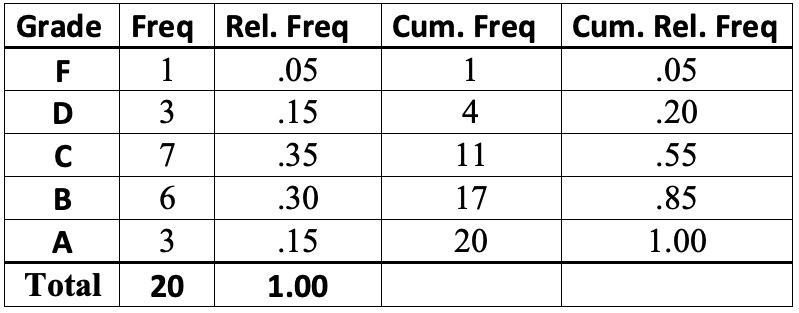
\includegraphics[width=0.6\linewidth]{week01/Grade-Freq-Table} \end{center}

\textbf{Remarks}: (1). The cumulative categories are defined to be F, D or below, C or below, etc. (2). For a nominal data, the cumulative frequency table may not be practically meaningful because the combined categories may not make practical sense.

\hypertarget{charting-categorical-data}{%
\subsection{Charting Categorical Data}\label{charting-categorical-data}}

Two major charts are used to characterize the distribution of a given categorical data set: bar chart and pie chart. Both chart are geometric representations of the frequency table discussed earlier.

\hypertarget{bar-chart}{%
\subsubsection{Bar Chart}\label{bar-chart}}

\textbf{Example 2:} We convert the frequency table of the course grade data in the following

\begin{center}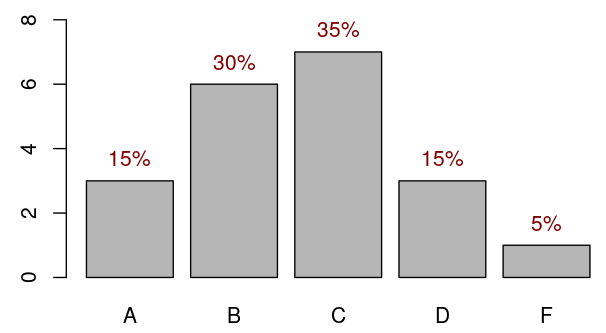
\includegraphics[width=0.6\linewidth]{week01/barChart} \end{center}

\textbf{Remark}: We can rearrange the vertical bars in ascending or descending order to get pare-to chart.

\begin{center}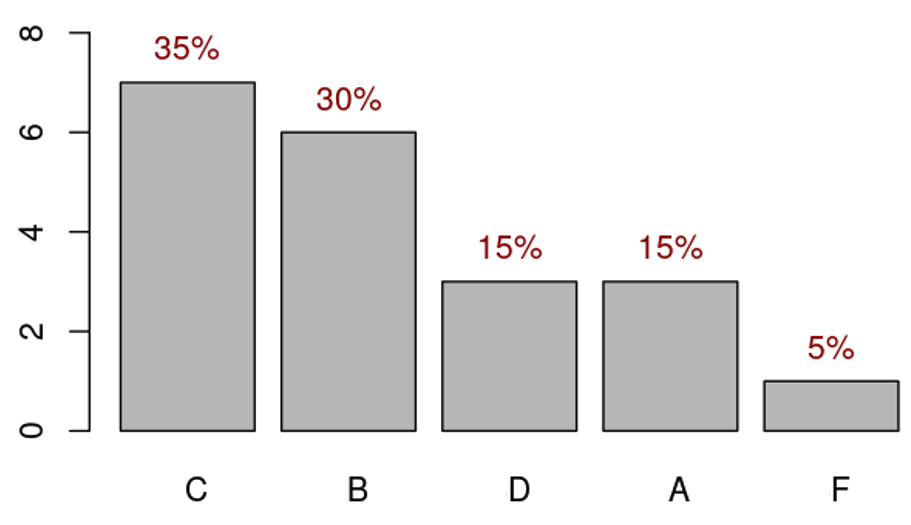
\includegraphics[width=0.6\linewidth]{week01/paretoChart} \end{center}

\hypertarget{pie-chart}{%
\subsubsection{Pie Chart}\label{pie-chart}}

To construct a pie chart manually, we need to calculate the degrees of the central angle of the circle and then slice it based on the degrees of the central angle.

\textbf{Example 3}: we still use the course grade frequency table (relative frequency) to to calculate the degrees of the corresponding central angle in the following table.

\begin{center}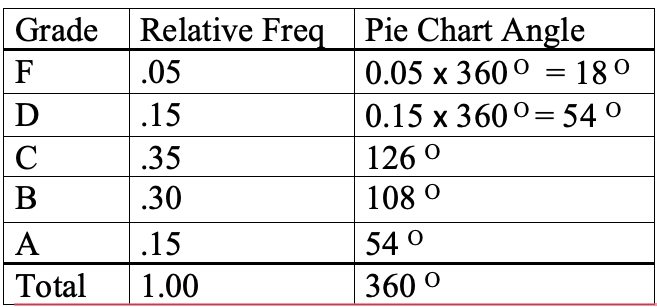
\includegraphics[width=0.5\linewidth]{week01/pieChartTable} \end{center}

The corresponding pie chart is given by

\begin{center}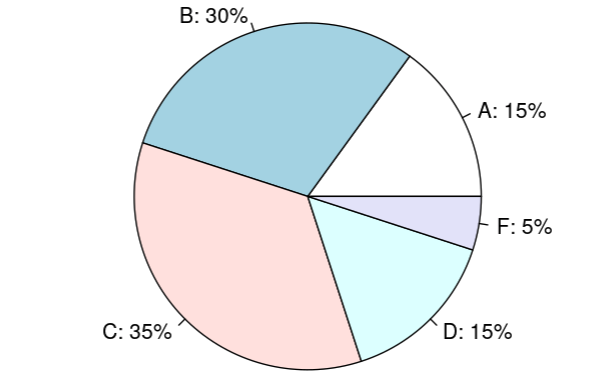
\includegraphics[width=0.5\linewidth]{week01/pieChart} \end{center}

\hypertarget{summary-of-numerical-data}{%
\section{Summary of Numerical Data}\label{summary-of-numerical-data}}

There are primarily two methods that are commonly used to summarize a given numerical data: Frequency tables and histograms.

\hypertarget{frequency-table}{%
\subsection{Frequency Table}\label{frequency-table}}

A histogram displays numerical data by grouping data into ``bins'' of equal width. Each bin is plotted as a bar whose height corresponds to how many data points are in that bin. Bins are also sometimes called ``intervals'', ``classes'', or ``buckets''.

There are several steps to follow when creating bins (with equal width):

\begin{itemize}
\item
  Determine the number of bins
\item
  Extend data window (from the smallest to the largest data values) if necessary to get ``convenient'' end values of the extended window. Caution: never shrink the data window because we must include all data values in one and only one of the bins!
\item
  Find the boundary values (cut-offs) so that all bins have equal width which is equal to \textbf{data-window-width/number-of-bins}.
\item
  The number of data values in each bin is the frequency of the bin.
\end{itemize}

\textbf{Example 4 - Length of CD: } Listed below are the lengths (in minutes) of randomly selected CDs of country, rock, and movie soundtracks.

\begin{verbatim}
20.5, 29, 32, 32, 32, 33, 36, 37, 38, 39, 39, 43, 47, 48, 49, 49, 49, 
50, 50, 51, 51, 52, 52, 52, 53, 54, 54, 54, 56, 56, 57, 58, 60, 61, 62, 
62, 69, 73, 74, 74.5 
\end{verbatim}

\textbf{Solution: } we follow the above suggested steps to define bins illustrated in the following figure.

\begin{center}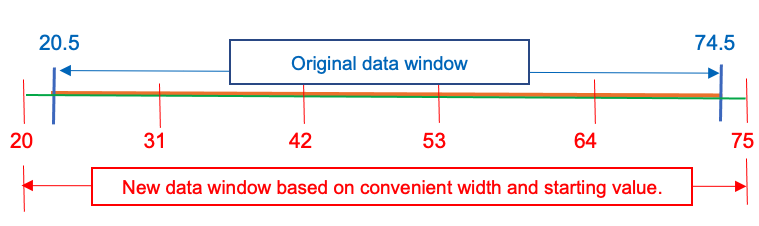
\includegraphics[width=0.8\linewidth]{week01/findingBins} \end{center}

\begin{itemize}
\item
  The number of bins chosen for this frequency table is 5.
\item
  The original data window is `{[}20.5, 74.5{]}'. The two end values are decimals. We extended the data window on both sides and get a an extended window {[}20, 75{]}.
\item
  The bin width = (75-20)/5 = 11.
\item
  The boundaries of the 5 bins are: 20, 31, 42, 53, 64, 75.
\item
  the five bins are: {[}20, 31{]}, (31, 42{]}, (42, 53{]}, (53, 64{]}, (64, 75{]}. Note that the boundary values must be included in one and only one bins. We use \texttt{"{[}"} and \texttt{")"} to denote inclusion and exclusion respectively. For example, in the second bin {[}31, 42), 31 is included in {[}31, 42) but 42 is NOT included in {[}31, 42). It is included in {[}42, 53).
\item
  with the above defined bins, the resulting frequency tables are given by
\end{itemize}

\begin{center}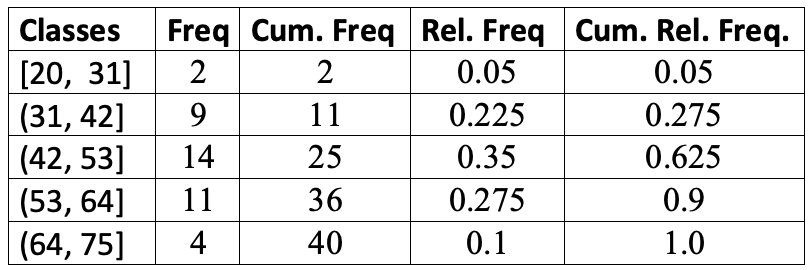
\includegraphics[width=0.6\linewidth]{week01/numFreqTable} \end{center}

\hypertarget{histogram}{%
\subsection{Histogram}\label{histogram}}

Similar to the bar chart and pie chat, a histogram is also a geometric representation of the frequency table constructed above. Since the bins are defined based on the numerical boundaries, they must be placed on the correct scales when constructing a histogram. This also means that the histogram is different from the bar chart in different perspectives:

\begin{itemize}
\item
  There is no gaps between the adjacent vertical bars because the horizontal axis is a numerical axis.
\item
  We cannot rearrange the vertical bars as we did in a bar chart to make a pareto chart since we cannot shuffle the boundaries on the numerical axis.
\end{itemize}

\textbf{Example 5 - Length of CD (cont'd):} The histogram based on the frequency table is given in the following.

\hfill\break

\hypertarget{exercises}{%
\section{Exercises}\label{exercises}}

Summarize the following data sets by using frequency tables (relative frequency, cumulative frequency, etc.) and histogram. You can use \texttt{IntroStatsApps} to check your work.

\textbf{Exercise 1}. Weights of 18- to 24- Year- Old Males. The U. S. National Center for Health Statistics publishes data on weights and heights by age and sex in the document Vital and Health Statistics. The weights shown in the following, given to the nearest tenth of a pound, were obtained from a sample of 18- to 24- year- old males. Use the cut-point grouping to organize these data into frequency and relative- frequency distributions. Use a class width of 20 and a first cut-point of 120.

\begin{verbatim}
129.2, 132.1, 136.7, 142.8, 145.6, 146.4, 149.9, 150.7, 151.3, 155.2, 
158.5, 158.6, 161.0, 161.7, 165.0, 165.8, 167.3, 170.0, 170.1, 172.5, 
173.6, 173.7, 175.4, 175.6, 178.2, 178.7, 182.0, 182.5, 185.3, 187.0, 
187.5, 188.7, 191.1, 209.1, 214.6, 218.1, 278.8
\end{verbatim}

\textbf{Exercise 2}. The following are the miles per gallon.

\begin{verbatim}
22.8, 22.9, 23.3, 23.4, 23.6, 23.7, 23.8, 23.9, 23.9, 24.1, 24.1, 24.2, 
24.3, 24.4, 24.5, 24.5, 24.6, 24.6, 24.7, 24.7, 24.7, 24.8, 24.8, 24.9, 
24.9, 25.0, 25.0, 25.1, 25.2, 25.3
\end{verbatim}

\textbf{Exercise 3}. Following are 80 measurements of the iron-solution index of tin-plate specimens, designed to measure the corrosion resistance of tin-plated steel. The original data set has been sorted in an ascending order as:

\begin{verbatim}
14,  26,  28,  28,  28,  28,  30,  32,  34,  35,  36,  36,  37,  37,  40, 
40,  40,  41,  41,  41,  42,  42,  42,  43,  43,  43,  44,  44,  44,  44,  
45, 45,  45,  45,  45,  45,  46,  46,  46,  46,  47,  47,  47,  48,  49,  
49,  49, 50,  50,  50,  51,  52,  52,  52,  52,  52,  53,  53,  54,  54,  
54,  54,  55, 55,  55,  55,  55,  55,  55,  56,  56,  56,  56,  56,  56,  
57,  57,  57,  57, 57,  58,  58,  58,  58,  58,  59,  59,  60,  60,  60,  
60,  61,  61,  61,  61, 61,  62,  62,  62,  62,  62,  62,  63,  63,  63,  
63,  63,  63,  64,  65,  66, 66,  67,  68,  68,  69,  69,  70,  70,  70,  
70,  70,  70,  71,  71,  72,  72, 72,  73,  74,  74,  74,  76,  76,  77,  
77,  79,  80,  81,  81,  83,  83,  84, 86,  86,  86,  87,  89,  92,  95
\end{verbatim}

\textbf{Exercises 4}. From the 140 children whose urinary concentration of lead were investigated 40 were chosen who were aged at least 1 year but under 5 years. The following concentrations of copper were found.

\begin{verbatim}
0.70, 0.45, 0.72, 0.30, 1.16, 0.69, 0.83, 0.74, 1.24, 0.77, 0.65, 0.76, 
0.42, 0.94, 0.36, 0.98, 0.64, 0.90, 0.63, 0.55, 0.78, 0.10, 0.52, 0.42,
0.58, 0.62, 1.12, 0.86, 0.74, 1.04, 0.65, 0.66, 0.81, 0.48, 0.85, 0.75, 
0.73, 0.50, 0.34, 0.88
\end{verbatim}

\textbf{Exercise 5} The following data set represents the shoe sizes of 100 random selected students from a large university.

\begin{verbatim}
8.0, 13.0, 8.5, 9.0, 11.0, 9.5, 10.0, 8.0, 11.0, 8.0, 10.0, 11.0, 10.0, 
11.0, 6.0, 9.0, 8.0, 8.0, 12.0, 10.5, 9.5, 11.0, 6.0, 8.0, 10.0, 11.5, 
11.0, 7.0, 10.5, 15.0, 12.0, 8.5, 8.0, 10.0, 8.0, 7.0, 10.5, 10.0, 5.0, 
7.0, 10.0, 14.0, 14.0, 8.5, 8.0, 13.0, 11.0, 6.0, 8.0, 11.5, 8.5, 7.0, 
12.5, 8.5, 15.0, 10.0, 6.0, 11.0, 11.0, 10.0, 10.5, 11.0, 7.5, 7.0, 7.5, 
10.5, 10.0, 11.0, 9.5, 11.0, 9.5, 10.5, 7.5, 11.0, 13.0, 10.0, 9.0, 12.0, 
8.0, 8.0, 9.0, 12.0, 8.5, 8.0, 11.0, 9.0, 9.0, 7.0, 9.0, 12.0, 5.5,
9.5, 8.0, 9.0, 12.0, 9.5, 9.0, 11.0, 13.0, 7.5
\end{verbatim}

\texttt{Caution}: The data values are given in the numeric form, but they are labels shoe sizes. Therefore, this is a categorical data set.

\hypertarget{use-of-technology}{%
\section{Use of Technology}\label{use-of-technology}}

In this class, I created several StatsApps to facilitate your learning of statistical concepts. The following screenshot gives the list of the available apps that cover about 90\% topics in this class.

\begin{center}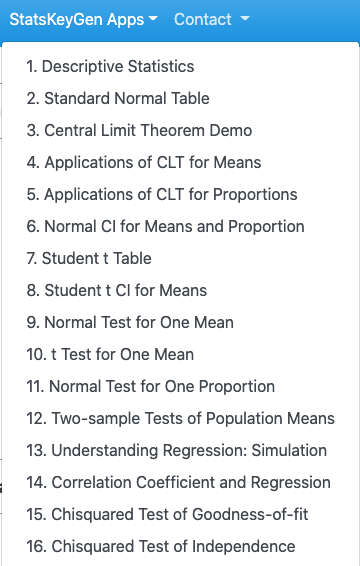
\includegraphics[width=0.3\linewidth]{week01/listApps} \end{center}

Next we use the first App to produce the answers to the two examples that we used in this note. The App can found at \url{https://wcupeng.shinyapps.io/DescriptiveStats/}. You need to type in data values and relevant information to generate frequency tables and charts.

\hypertarget{course-grade-data}{%
\subsection{Course Grade Data}\label{course-grade-data}}

The following show the frequency table generated from the App using the course letter grades. You can try to generate bar charts and pie charts using this app.

\begin{center}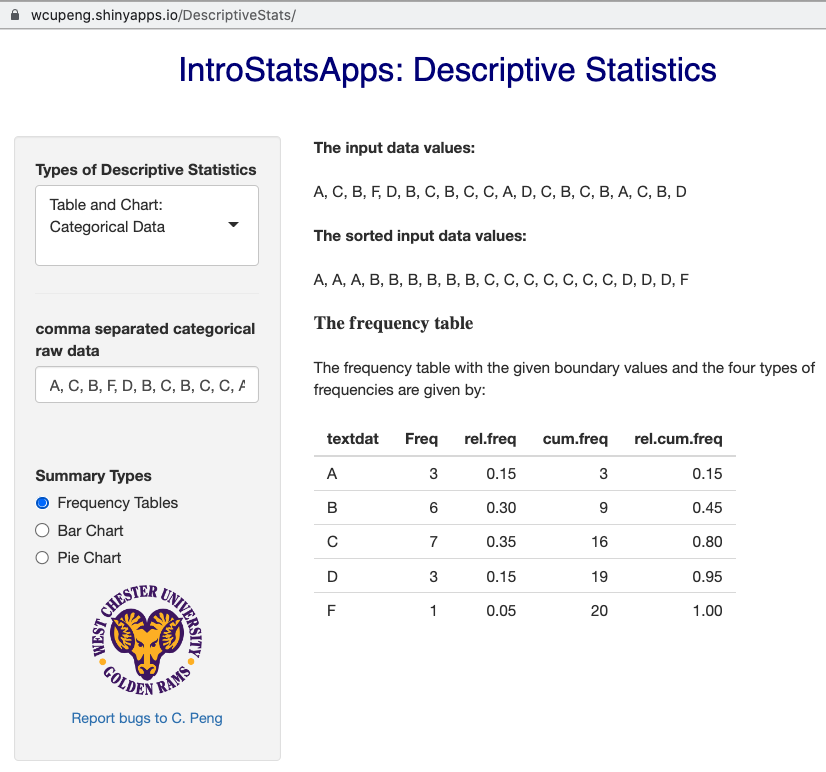
\includegraphics[width=0.8\linewidth]{week01/cateFreq} \end{center}

\hypertarget{length-of-cd-data}{%
\subsection{Length of CD data}\label{length-of-cd-data}}

The following show the frequency table generated from the App using the length of CD data in the example. You can try to generate histograms using this app. Please keep in mind the boundary values MUST be provided to obtain the appropriate frequency tables and histograms.

\begin{center}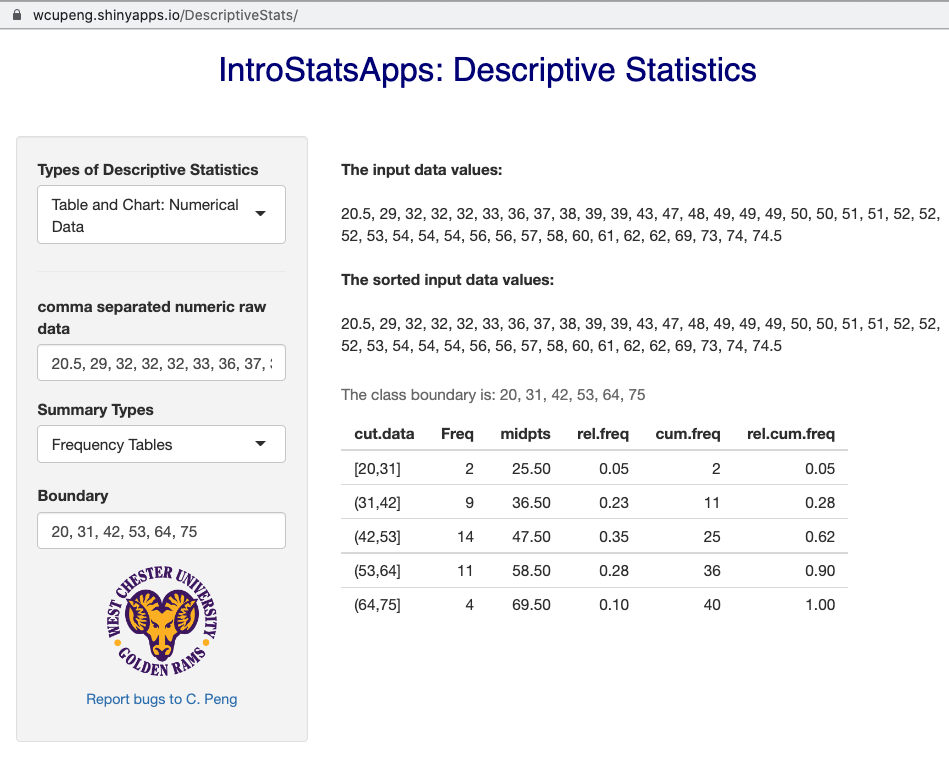
\includegraphics[width=0.8\linewidth]{week01/numFreq} \end{center}

\hypertarget{numerical-measures}{%
\chapter{Numerical Measures}\label{numerical-measures}}

This note focuses on using numerical measures to characterize numerical data sets. The numerical measures are used to describe the features such as mean, variance, and percentiles of a given numerical data set. These numeric measures are classified into three categories: central tendency, variation, and locations.

\hypertarget{notations-using-greek-letters-for-parameters}{%
\section{Notations Using Greek Letters for Parameters}\label{notations-using-greek-letters-for-parameters}}

Every data set has a name. For example, the set of heights of a group of WCU students is a data set that can be named \texttt{h} or \texttt{height}. We can give each data value has a ``generic name'' such as \(h_1, h_2, \cdots, h_5\), etc. The following figure gives other examples of generic names of values in different data sets.

\begin{center}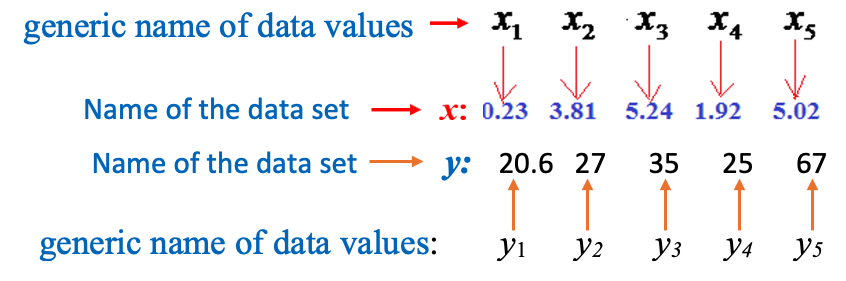
\includegraphics[width=0.6\linewidth]{week02/genericNames} \end{center}

\hypertarget{big-sigma-sigma-notation}{%
\subsection{\texorpdfstring{Big Sigma (\(\Sigma\)) Notation}{Big Sigma (\textbackslash Sigma) Notation}}\label{big-sigma-sigma-notation}}

These ``generic names'' were used to make compact formulas in some numeric measures. The sum of all data values in the data set with the name x (in the above figure) is given by the following \textbf{big sigma} notation.

\begin{center}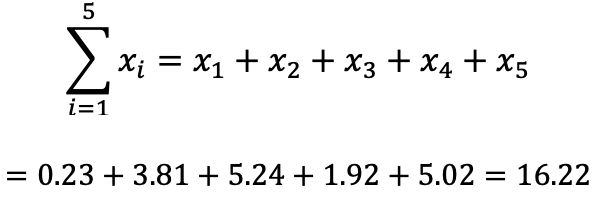
\includegraphics[width=0.5\linewidth]{week02/bigSigmaNotation} \end{center}

\textbf{Example 1}: Consider the following two data sets with names \textbf{x} and \textbf{y}, we want to take the product of the corresponding values and sum up the product of the corresponding values. The following is the \textbf{big sigma} notation of the \textbf{sum of the cross-product}.

\begin{center}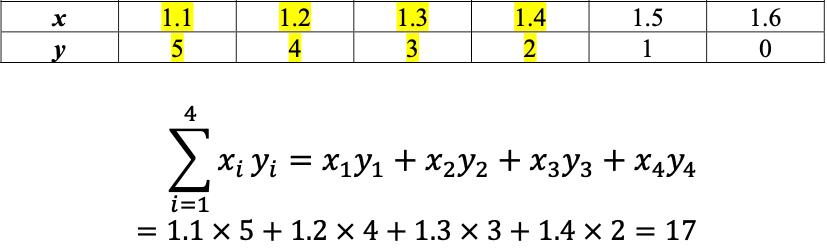
\includegraphics[width=0.7\linewidth]{week02/crossProductNotation} \end{center}

\hypertarget{notations-for-parameters-and-statistics}{%
\subsection{Notations for Parameters and Statistics}\label{notations-for-parameters-and-statistics}}

We use Greek letters to denote the population parameters of populations and English letters to denote statistics from the samples.

\begin{center}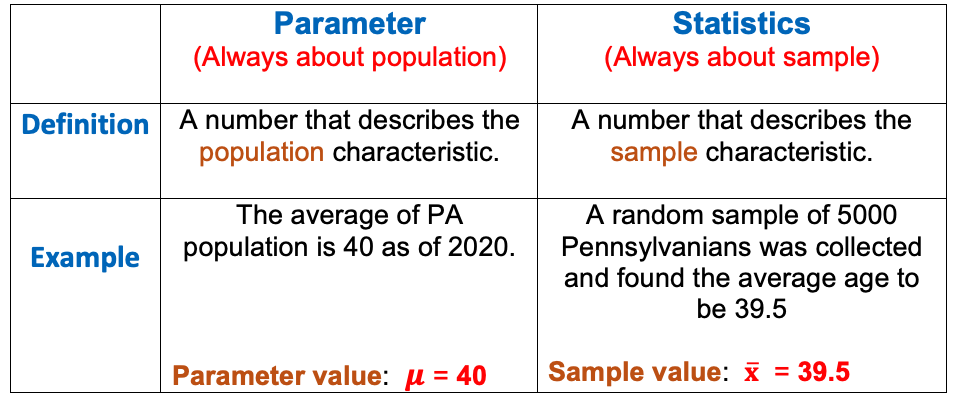
\includegraphics[width=0.7\linewidth]{week02/samplePopMeans} \end{center}

\hfill\break

\hypertarget{measures-of-center}{%
\section{Measures of Center}\label{measures-of-center}}

Three measures are used as the center of a given numeric data set.

\begin{center}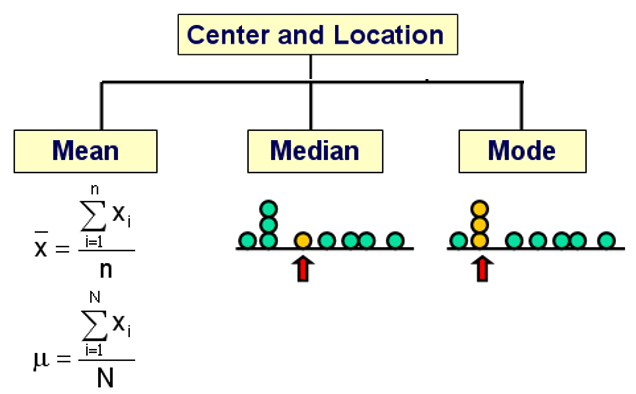
\includegraphics[width=0.6\linewidth]{week02/measuresOfCenter} \end{center}

\hypertarget{mean}{%
\subsection{Mean}\label{mean}}

The mean of a given data set is defined as the average of all data values. The big sigma notations of sample and population means are given by

\begin{center}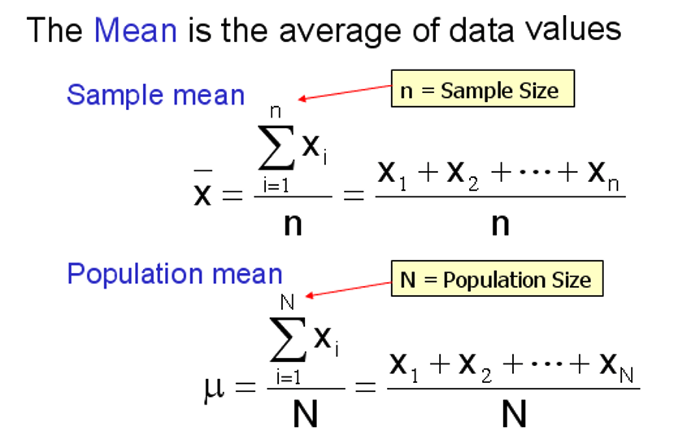
\includegraphics[width=0.5\linewidth]{week02/mean} \end{center}

\textbf{Remark}: the mean can be affected significantly by outliers (extreme values). For example,

\hypertarget{median}{%
\subsection{Median}\label{median}}

The middle value of a sorted data set is called the median of the data set.

\begin{itemize}
\item
  If a data set has an \textbf{odd number} of data values, there is a unique ``middle'' value in the \textbf{sorted data} set.
\item
  If a data set has an \textbf{even number} of data values, there will be two \textbf{middle} values in the \textbf{sorted data} set, in this case, the \textbf{average} of the two ``middle** values is defined to be the median.
\end{itemize}

For example,

\begin{itemize}
\item
  \{2, 6, 7\} \(\to\) median = 6
\item
  \{1, 2, 6, 7\} \(\to\) median = (2 + 6) / 2 = 4.
\end{itemize}

\hypertarget{mode}{%
\subsection{Mode}\label{mode}}

The mode(s) is (are) the data value(s) with highest frequency.

\begin{itemize}
\tightlist
\item
  If there is only one mode, the data set is unimodal.
\item
  If there are two modes, the data set is bimodal.
\item
  If there are more than two modes, the data is multi-modal.
\end{itemize}

\begin{center}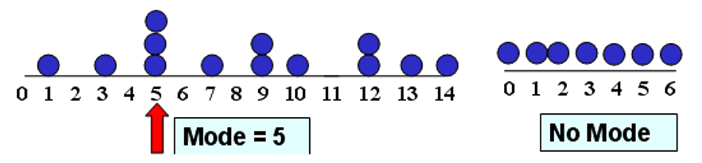
\includegraphics[width=0.55\linewidth]{week02/mode} \end{center}

\hypertarget{relationship-between-mean-median-and-mode}{%
\subsection{Relationship between Mean, Median, and Mode}\label{relationship-between-mean-median-and-mode}}

The relationship between mean, median, and mode is dependent on the shape of the distribution. The following figure illustrates this relationship.

\begin{center}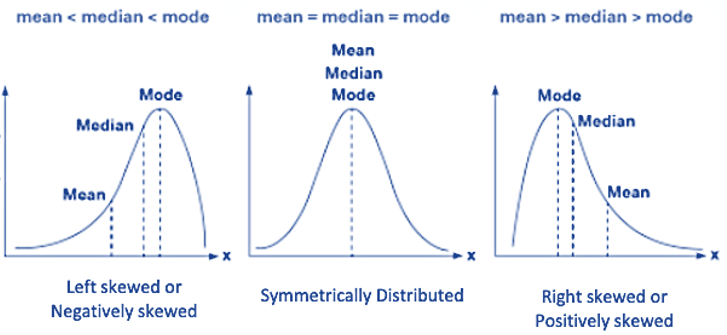
\includegraphics[width=0.7\linewidth]{week02/skewness} \end{center}

\hypertarget{measures-of-variation}{%
\section{Measures of Variation}\label{measures-of-variation}}

Measures of variation are used to characterize the shape of the distribution. There are some different measures used in different situations. We only introduce the variance and the standard deviation in this course. We will also briefly introduce IQR in the applications of numerical measures.

\hypertarget{variance}{%
\subsection{Variance}\label{variance}}

Since the definitions of sample and population variances are different, we need to choose an appropriate formula based on whether the data set is a population or a sample. This information is provided to you before you select a formula to calculate the variances. The exact definitions using big sigma notation are given below

\begin{itemize}
\tightlist
\item
  Population Variance
\end{itemize}

\[
\sigma^2 = \frac{\Sigma_{i=1}^N (x_i-\mu)^2}{N}=\frac{(x_1-\mu)^2 + (x_2-\mu)^2+\cdots+(x_N-\mu)^2}{N}
\]

\begin{itemize}
\tightlist
\item
  Sample Variance
\end{itemize}

\[
s^2 = \frac{\Sigma_{i=1}^n (x_i-\bar{x})^2}{n-1}=\frac{(x_1-\bar{x})^2 + (x_2-\bar{x})^2+\cdots+(x_n-\bar{x})^2}{n-1}
\]

We can see the only difference is in the denominator of the two definitions.

\hypertarget{standard-deviation}{%
\subsection{Standard Deviation}\label{standard-deviation}}

Once the variance is calculated, we simply take the square root to obtain the standard deviation

\begin{itemize}
\tightlist
\item
  Population standard deviation
\end{itemize}

\[
\sigma = \sqrt{\frac{\Sigma_{i=1}^N (x_i-\mu)^2}{N}} = \sqrt{\frac{(x_1-\mu)^2 + (x_2-\mu)^2+\cdots+(x_N-\mu)^2}{N}}
\]

\begin{itemize}
\tightlist
\item
  Sample Standard Deviation
\end{itemize}

\[
s = \sqrt{\frac{\Sigma_{i=1}^n (x_i-\bar{x})^2}{n-1}}=\sqrt{\frac{(x_1-\bar{x})^2 + (x_2-\bar{x})^2+\cdots+(x_n-\bar{x})^2}{n-1}}
\]

\hypertarget{steps-for-calculating-variance}{%
\subsection{Steps for Calculating Variance}\label{steps-for-calculating-variance}}

The following are steps for calculating the variance of a data set.

\begin{center}\includegraphics[width=0.65\linewidth]{week02/calcVariance} \end{center}

\textbf{Example 2} The following table illustrates how to use the above steps to calculate the variance of a small \textbf{sample} toy data set: A = \{1,4,7\}.

\begin{center}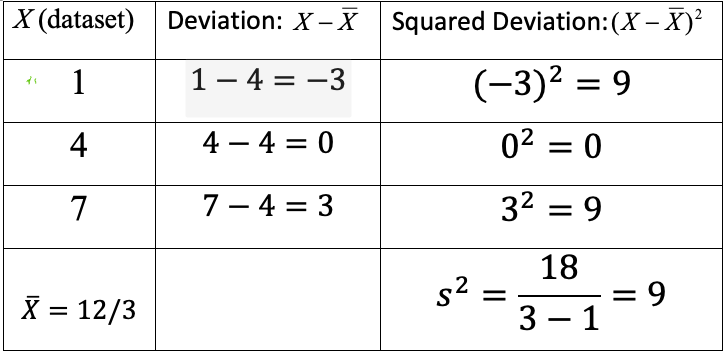
\includegraphics[width=0.55\linewidth]{week02/varCalc} \end{center}

Based on the above table, we can see that the standard deviation is \(\sqrt{9} = 3\) .

\hypertarget{measures-of-location}{%
\section{Measures of Location}\label{measures-of-location}}

Two important types of measures of location will be introduced in this course: z-score and percentiles.

\hypertarget{z-score}{%
\section{z-score}\label{z-score}}

A Z-score of a value of a \textbf{sample} data set is a standardized score that is defined by

\[
z = \frac{x - \bar{x}}{s}.
\]

We can easily adjust the above formula for a population as

\[
z = \frac{x - \mu}{\sigma}.
\]
\textbf{Example 3}: We still use the same sample toy data, A = \{1,4,7\}, used in \textbf{Example 2} to illustrate how to find z-scores of corresponding data values.

\textbf{Solution: } We know from \textbf{Example 2} that \(\bar{x} = 4\) and \(s = 3\). Therefore, the z-scores of the corresponding data values are calculated in the following.

\(x_1 = 1 \to z_1 = \frac{1 - 4}{3} = -1\)

\(x_2 = 4 \to z_2 = \frac{4 - 4}{3} = 0\)

\(x_3 = 7 \to z_3 = \frac{7 - 4}{3} = 1\)

That is, the standardized set of z-scores is \(\{ -1, 0, 1\}\). Note this is a set of sample z-scores. We can easily verify that the mean and standard deviation of the above three z-scores are 0 and 1 respectively.

\hypertarget{percentile}{%
\subsection{Percentile}\label{percentile}}

A \textbf{percentile} indicates the percentage of scores that fall below a particular value.

\textbf{Example 4} Consider the following PSAT percentile table.

\begin{center}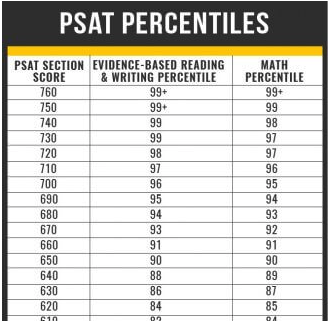
\includegraphics[width=0.45\linewidth]{week02/percentileChart} \end{center}

If you took PSAT and scored 640 in the MATH section, according to the above table, your MATH percentile is 89\% meaning that 89\% of all examinees scored below 640 in the PSAT. This also means that you did better than 89\% of your peers on the PSAT.

\textbf{Steps for Calculating Percentiles}

Assume that we have a data set \(\{ x_1, x_2, \cdots, x_n \}\). we want to find \(k-th\) percentile, denoted by \(P_k\).

\textbf{Step 1:} Sort the data in ascending order: \(\{ x_{(1)}, x_{(2)}, \cdots, x_{(n)} \}\).

\textbf{Step 2:} Calculate the \texttt{rough\ location} of the \(k-th\) percentile
\[L = \frac{k}{100}\times n.\]

\textbf{Step 3:} The \(k^{th}\) percentile is obtained depending on the form of \(L\).

\begin{itemize}
\item
  if \(L\) is a whole number, then the \(k^{th}\) percentile is the average of the number in position \(L\) and the number in position \(L+1\) in the sorted data set.
\item
  if \(L\) is NOT a whole number, round it \textbf{up} to the next higher whole number. The \(k^{th}\) percentile is the number in the position corresponding to the \textbf{rounded-up} value.
\end{itemize}

\textbf{Example 5:} Consider the following data set

\begin{verbatim}
9, 13, 7, 7, 12, 15, 10, 10, 6, 19, 17, 10, 15, 9, 14, 12, 9, 13, 7, 
7, 4, 8, 19, 5, 18, 20, 14, 1, 23, 10, 10, 7, 22, 9, 1
\end{verbatim}

Find \(P_{40}\) and \(P_{55}\) percentiles respectively.

\textbf{Solution} we first sort the data in ascending order.

\begin{verbatim}
1, 1, 4, 5, 6, 7, 7, 7, 7, 7, 8, 9, 9, 9, 9, 10, 10, 10, 10, 10, 12, 12,
13, 13, 14, 14, 15, 15, 17, 18, 19, 19, 20, 22, 23
\end{verbatim}

\textbf{To find 40th percentile},

\[
L = \frac{40}{100}\times 35 = 14.
\]
Since \(L = 14\) is an integer, the 20th percentile is the average of 14th and 15th data values in the sorted data set. That is, (9 + 9)/2 = 9.

\textbf{To find 55th percentile},

\[
L = \frac{55}{100}\times 35 = 19.25.
\]

Since \(L=19.25\) is NOT an integer, we round up L to get \textbf{20}. The 55th percentile is the 20th data value in the sorted data set which is 10.

\hypertarget{applications-of-numeric-measures}{%
\subsection{Applications of Numeric Measures}\label{applications-of-numeric-measures}}

Three concepts based on the numeric measures will be introduced in the following.

\hypertarget{five-number-summary}{%
\subsubsection{Five Number Summary}\label{five-number-summary}}

The five number summary consists of the minimum, 25th, 50th, 75th percentiles, and the maximum. The 25th, 50th, and 75th percentiles are also called the first (\(Q_1\)), second (\(Q_2\)) and third quartiles (\(Q_3\)), respectively.

\textbf{Example 6: } We use the \textbf{length of CD} data to show the five-number-summary. The unit of data values is minute. The following is the sorted data.

\begin{verbatim}
20.5, 29, 32, 32, 32, 33, 36, 37, 38, 39, 39, 43, 47, 48, 49, 49, 49, 
50, 50, 51, 51, 52, 52, 52, 53, 54, 54, 54, 56, 56, 57, 58, 60, 61, 62, 
62, 69, 73, 74, 74.5 
\end{verbatim}

\textbf{Solution}, The minimum and maximum are 20.5 and 74.5 minutes. The quartiles are calculated in the following.

\(Q_1: L = (25/100) \times 40 = 10\), \(Q_1\) is the average of the 10th and 11th data values \(= (39+39)/2 = 39\).

\(Q_2: L = (50/100) \times 40 = 20\), \(Q_1\) is the average of the 20th and 21st data values \(= (51 + 51)/2 = 51\).

\(Q_3: L = (75/100) \times 40 = 30\), \(Q_1\) is the average of the 30th and 31st data values \(= (56+57)/2 = 56.5\).

Therefore, the five-number-summary is given by

\begin{verbatim}
     Min      Q1       Q2        Q3        Max
    20.5      39       51       56.5       74.5
\end{verbatim}

\hypertarget{box-plot}{%
\subsubsection{Box-plot}\label{box-plot}}

The box-plot is a geometric representation of the five-number-summary given in the following figure

\begin{center}\includegraphics[width=0.6\linewidth]{week02/boxPlot} \end{center}

Box-plots are used to describe the distribution of data. The following three box-plots represent three different types of distributions:

\begin{center}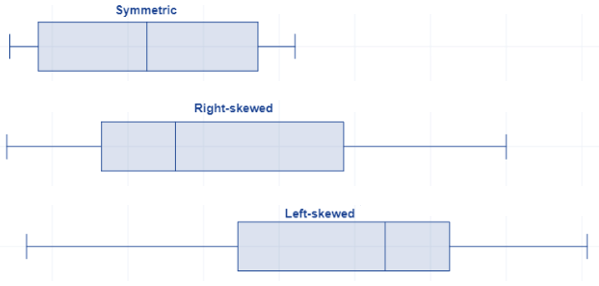
\includegraphics[width=0.6\linewidth]{week02/interpretationBoxPlot} \end{center}

\textbf{Example 7: (Length of CS Continued)} The box-plot is given by

\begin{center}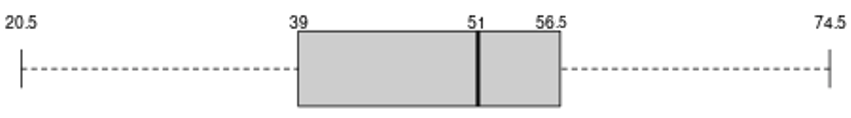
\includegraphics[width=0.7\linewidth]{week02/boxPlotExample} \end{center}

\hypertarget{inter-quartile-range-iqr}{%
\subsubsection{Inter-quartile Range (IQR)}\label{inter-quartile-range-iqr}}

The inter-quartile range of data is defined by \(IQR = Q3 - Q1\). IQR is used to measure the variation of the data set. It is NOT sensitive to extremely large and small values since IQR is defined only based on the ``middle 50\% of data values''.

\begin{center}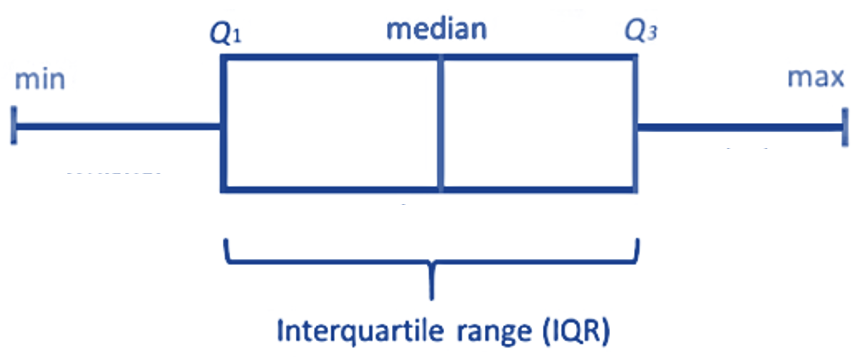
\includegraphics[width=0.55\linewidth]{week02/IQR} \end{center}

\hfill\break

\hypertarget{use-of-technology-1}{%
\section{Use of Technology}\label{use-of-technology-1}}

We still use the same app that we used in the previous note to find various numerical measures to summarize a given data set. The app can be found at \url{https://wcupeng.shinyapps.io/DescriptiveStats/}. The next screenshot illustrates the measures of variations in the length of CD data. You can choose to find other numerical measures of the data.

\begin{center}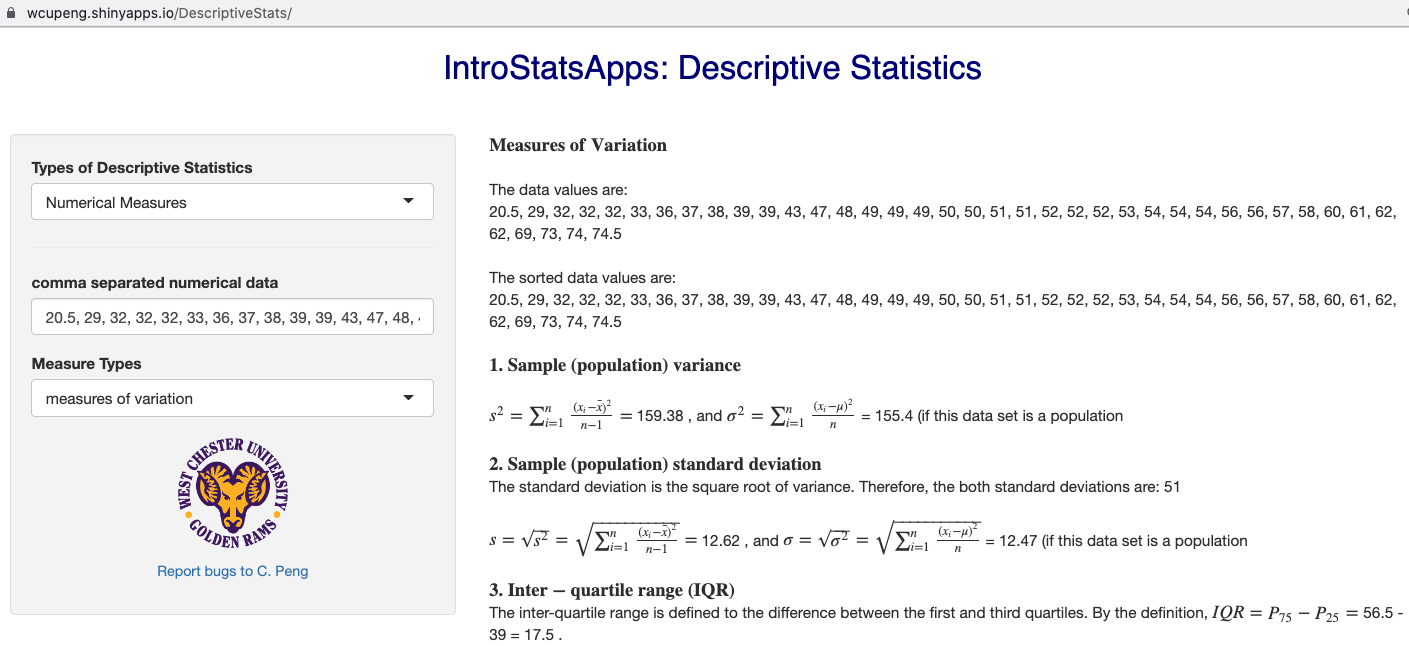
\includegraphics[width=0.95\linewidth]{week02/techSpread} \end{center}

\hypertarget{concepts-of-probability}{%
\chapter{Concepts of Probability}\label{concepts-of-probability}}

\hfill\break

\textbf{Q}: Why do we need to study probability?

\textbf{A}: We can build a bridge between a sample and its population so that one can make inferences about the population from its samples.

In this note, we introduce the definitions of probability, random variables, and problems associated with a distribution based on a special distribution: uniform distribution.

\hypertarget{definitions-of-probability}{%
\section{Definitions of Probability}\label{definitions-of-probability}}

We need to use the following concepts to define or approximate the probability of an event.

\hypertarget{experiment-and-event}{%
\subsection{Experiment and Event}\label{experiment-and-event}}

\textbf{An experiment} is any process that generates well-defined outcomes. On any single repetition of an experiment, one and only one of the possible experimental outcomes will occur.

Example 1. The following table gives several examples of experiments.

\begin{center}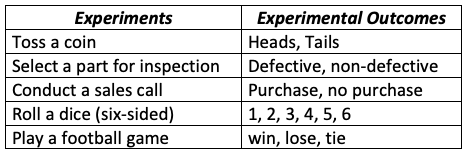
\includegraphics[width=0.55\linewidth]{week03/experiments} \end{center}

\textbf{The Sample Space} of an experiment is the set of all possible outcomes. We usually use a capital letter in Greek or English to denote the sample space. For example, \(\Omega\), \(S\), or \(U\).

Example 2. Consider the experiment of tossing a balanced coin sequentially for 2 times. We use H to denote the heads and T to denote the tails.

\begin{center}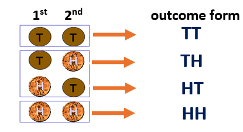
\includegraphics[width=0.4\linewidth]{week03/coinTossing} \end{center}

Therefore, the sample space of this experiment is \(\Omega = \{ TT, TH, HT, HH \}\).

\textbf{An Event} is a subset of outcomes from the sample space. We usually use a capital letter to denote an event.

Example 3. We define Event E to be at least one H is observed in the coin tossing example.

\textbf{Solution: } The outcomes in the subset \(\{HT, TH, HH\}\) satisfy the requirement in the definition. Therefore, event E is defined by \(E = \{ HT, TH, HH\}\).

\hypertarget{definition-of-probabilities}{%
\section{Definition of Probabilities}\label{definition-of-probabilities}}

\textbf{Notations: } We use \(P\) or \(Pr\) to denote the probability and \(A, B, C, \cdot,\) to denote specific events. \(P(A)\) is the probability that event A occurs.

\hypertarget{definitions-of-probability-1}{%
\subsection{Definitions of Probability}\label{definitions-of-probability-1}}

\begin{itemize}
\tightlist
\item
  \textbf{Method 1:} Relative Frequency Approximation of Probability.
\end{itemize}

Conduct or observe an experiment a large number of times and count the number of times that event A occurs. Based on these actual results, P(A) is estimated as follows:

\begin{verbatim}
            P(A)= (# of times of A being observed) / (# of repeated trials)
\end{verbatim}

\begin{itemize}
\tightlist
\item
  \textbf{Method 2:} Classical Approach to Probability (Requires Equally Likely Outcomes of the experiment)
\end{itemize}

\begin{verbatim}
              P(A) = (# of outcomes in A) / (# of outcome in S) 
\end{verbatim}

\hypertarget{some-examples}{%
\subsection{Some Examples}\label{some-examples}}

Example 4. \textbf{Guessing Answers on an ACT:} A typical multiple-choice question has 5 possible answers. If you make a random guess on one question, what is the probability that your response is wrong?

\textbf{Solution}: Method 2 classical approach applies to this question since each of the choices is random, that is, each of the 5 letters A, B, C, D, and E are equally likely to be selected as the correct answer.

\begin{verbatim}
                Pr(wrong answer) = 4 / 5 =0.8
\end{verbatim}

\hfill\break

Example 5. \textbf{Gender of Children}: Find the probability that a randomly selected couple with 3 children will have exactly 2 boys. Assume that boys and girls are equally likely, and the gender of any child is not influenced by the gender of any other child.

\textbf{Solution} Based on the given condition, this is an equally likely experiment. We first use a table to list all possible outcomes in the sample space. Let B = boy and G = girl. Then the following table lists all possible outcomes of this experiment.

\begin{center}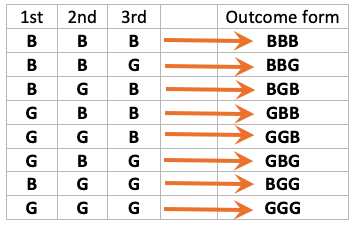
\includegraphics[width=0.4\linewidth]{week03/threeKidFamily} \end{center}

We list the sample space as follows

\begin{verbatim}
                S = { BBB   BBG   BGB   GBB   GGB   GBG   BGG   GGG }
                E =  having exactly 2 boys = { BBG   BGB   GBB }. 
\end{verbatim}

The desired probability can be calculated as

\begin{verbatim}
                     Pr(E)= #E/#S  = 3 / 8 =0.375.
\end{verbatim}

\hypertarget{discrete-probabilities-on-contingency-tables}{%
\subsection{Discrete Probabilities on Contingency Tables}\label{discrete-probabilities-on-contingency-tables}}

Contingency tables classify outcomes in rows and columns. Table cells at the intersections of rows and columns indicate frequencies of both events coinciding.

Example 6. The following table displays events for computer sales at a fictional store.

\begin{center}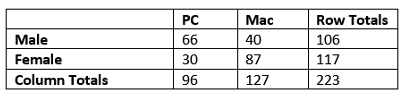
\includegraphics[width=0.5\linewidth]{week03/contingencyTable} \end{center}

Specifically, it describes the frequencies of sales by the customer's gender and the type of computer purchased. The cells' counts represent the number of PCs and Macs purchased by both genders.

Finding the following probabilities:

(1). Randomly select a female customer, what is the probability that she bought a Mac computer?

(2). Randomly select a customer from those who bought a computer from the store, what is the probability that the customer is a male?

(3). Randomly select a customer who bought a computer from the store, what is the probability she/he bought a Windows computer?

(4). Randomly select a customer who bought a computer from the store, what is the probability that the customer is female and bought a Mac computer?

\textbf{Solution} (1). \(P\)(Mac among female) \(= 87/117 = 0.744\)

(2). \(P\)(male among customers who bought a computer) \(= 106/223 = 0.4753\)

(3). \(P\)(windows among all computers sold) \(= 96/223 = 0.4305\)

(4). \(P\)(female \& bought a mac computer) \(= 87/223 = 0.3901\)

\hypertarget{concepts-of-random-variables}{%
\section{Concepts of Random Variables}\label{concepts-of-random-variables}}

\textbf{Random Variable (informal description)}: A random variable is a numerical description of the outcome of an experiment, its value depends on chance.

Example 7. Let Y be a variable denoting the height of WCU students. Before you measure the height of a selected student, Y is unknown. Furthermore, the unknown value is dependent on the chance since selecting a student involves uncertainty! This type of variable is a random variable.

\textbf{Characterization of Random Variables}: We study the behavior of a random variable through its probability distribution function.

\textbf{Use of Random Variables}: We use random variables to characterize the random behavior of real-world problems to inform statistical decisions using probability distributions.

\textbf{Classification of Random Variables}

\begin{center}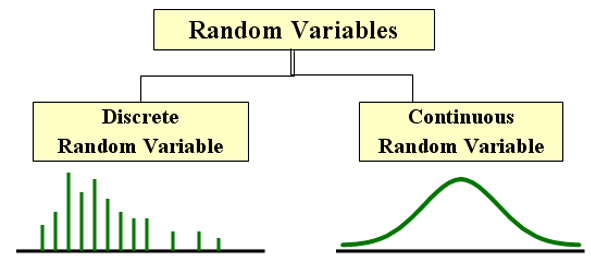
\includegraphics[width=0.5\linewidth]{week03/classificationRV} \end{center}

\hypertarget{discrete-random-variable}{%
\subsection{Discrete Random Variable}\label{discrete-random-variable}}

\textbf{Discrete Random Variable:} A discrete random variable may assume either a finite number of values or an infinite sequence of values such as 1, 2, \ldots, etc.

Example 8. The following table gives several example of discrete random variables.

\begin{center}\includegraphics[width=0.6\linewidth]{week03/discreteRV} \end{center}

We use the probability distribution to characterize a random variable. For convenience, we use a capital letter (such as \(X\)) to denote the name of the random variable and a lower-case letter (\(x\)) to denote the value of the random variable,

\textbf{The probability distribution} of a discrete random variable is a graph, table, or formula that gives the probability for each value of the random variable. For a probability distribution, the following requirements MUST be satisfied.

\begin{enumerate}
\def\labelenumi{\arabic{enumi}.}
\item
  \(\sum P(x) = 1\), where \(x\) assumes all possible values of random variable \(X\).
\item
  \(0 \le P(x) \le 1\), for every value of \(x\).
\end{enumerate}

\textbf{Defining Events Based on Values of A Random Variable}

An event defined based on a discrete random variable is a subset of the collection of all possible values of the discrete random variable!

\hfill\break

Example 9.. Let's consider the experiment of tossing a balanced coin two times. The sample space \(\Omega = \{ TT, TH, HT, HH \}\). We can define a random variable \(X=\) number of \textbf{heads} observed in an experiment.

As an illustration, we define several events based on the above random variable based on various values in the following.

\begin{verbatim}
      E1 = {X = 1} = (TH, HT) ,  then   P(E1) = 2/4 = 0.5
      E2= {X>0} ={TH, HT, HH},   then  P(E2) = 3/4
      E3 = {X !=1} = {HH, TT},   then    P(E3) = 2/4 = 0.5
\end{verbatim}

The complete probability distribution is outlined in the following figure.

\begin{center}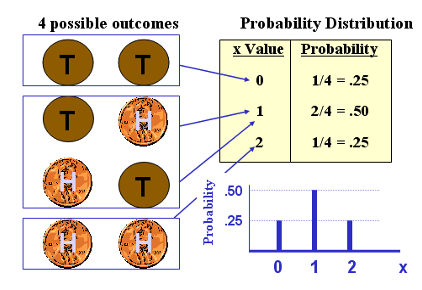
\includegraphics[width=0.5\linewidth]{week03/coinTossingRV} \end{center}

The top-right table is the probability distribution table, and the bottom right is the probability distribution table (geometric representation of the probability distribution table).

Example 10.. \textbf{Gender of Children} If a couple plans to have 3 children. Let \(X =\) the number of sons they may have. What is the probability distribution of \(X\)?

\textbf{Solution:} The possible values of the R.V. X are 0, 1, 2, and 3 which correspond to the four events. Using the definition of class probability, we have Pr(X =0 ) = 1/8, Pr(X = 1) = 3/8, Pr(X = 2) = 3/8 and Pr(X = 3) = 1/8. So, we have the following probability distribution table.

\begin{center}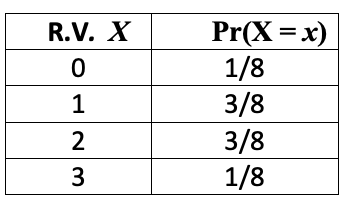
\includegraphics[width=0.3\linewidth]{week03/probDist3Kid} \end{center}

The probability distribution histogram is given by

\begin{center}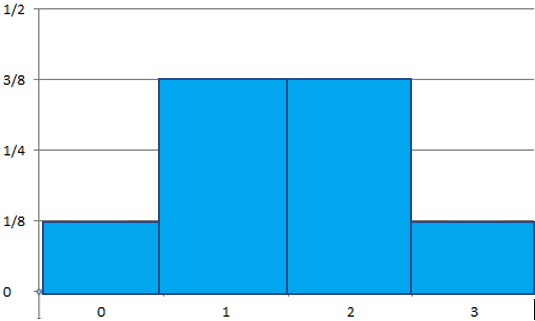
\includegraphics[width=0.4\linewidth]{week03/probHist3Kid} \end{center}

\hfill\break

\hypertarget{continuous-random-variable-and-density-functions}{%
\subsection{Continuous Random Variable and Density Functions}\label{continuous-random-variable-and-density-functions}}

A continuous random variable takes on uncountably infinite values. For example, body temperatures, height, weight, etc.

As opposed to the discrete variables that could be characterized by a probability table or a probability function, for a continuous random variable, we use the probability density function to characterize the distribution.

The probability density function of \(Y\), denoted by \(f(y)\), MUST satisfy the following two conditions that are analogous to the two requirements in the probability distribution function:

\begin{enumerate}
\def\labelenumi{(\arabic{enumi})}
\item
  a non-negative real-valued function is defined on all the real numbers, and such that
\item
  the area between the curve and the horizontal axis is equal to 1.
\end{enumerate}

\begin{center}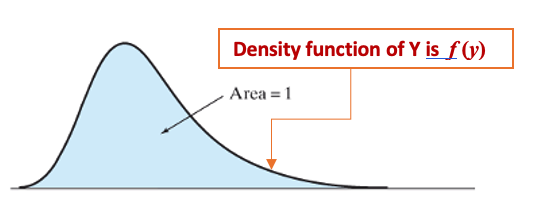
\includegraphics[width=0.5\linewidth]{week03/densityCurve} \end{center}

\hfill\break

\textbf{Definition of Events Using Continuous Variables}

An event defined based on a continuous random variable is one or more intervals of values of the continuous random variable. The probability of the event is equal to the area between the density curve and the interval(s).

The following figure illustrates the definition of an event and its corresponding probability.

\begin{center}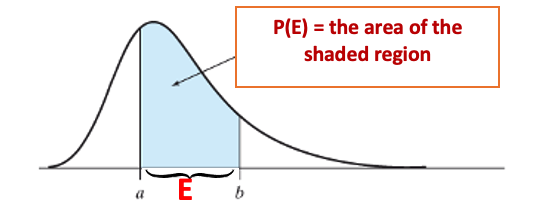
\includegraphics[width=0.5\linewidth]{week03/eventContRVProb} \end{center}

Since the \texttt{area} of a line segment is zero, the probability that a continuous random variable exactly equals any value is always zero.

\hypertarget{uniform-random-variable---a-special-continuous-distribution}{%
\section{Uniform Random Variable - A Special Continuous Distribution}\label{uniform-random-variable---a-special-continuous-distribution}}

A uniform distribution, also called a rectangular distribution, is a probability distribution that has constant probability. The general formula for the probability density function (pdf) for the uniform distribution is

\begin{center}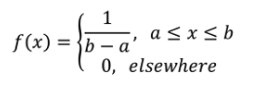
\includegraphics[width=0.3\linewidth]{week03/uniformDensityFun} \end{center}

The density curve is given by

\begin{center}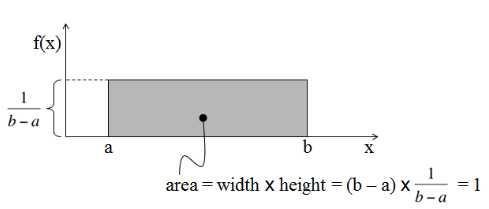
\includegraphics[width=0.55\linewidth]{week03/uniformDensityCurve} \end{center}

Example 11.. Consider the following function defined on interval {[}1,9{]}.

\begin{center}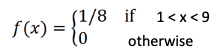
\includegraphics[width=0.3\linewidth]{week03/uniformExample01} \end{center}

Is \(f(x)\) a valid density function of the uniform distribution?

\textbf{Solution}: We only need to check whether the two requirements of continuous density functions are satisfied.

\begin{enumerate}
\def\labelenumi{\arabic{enumi}.}
\item
  \(f(x) \ge 0\) for all \(x\);
\item
  The area between the density curve and the horizontal axis is equal to 1, This is obvious from the following density curve.
\end{enumerate}

Therefore,

is a valid density function.

Example 11.. A shuttle train at a busy airport completes a circuit between two terminals every five minutes. Answer the following questions with the assumption that passengers arrive at a stop at any time in a 5-minute time window (we could assume a uniform arrival time).

\begin{enumerate}
\def\labelenumi{\arabic{enumi})}
\item
  What is the probability that a passenger will wait for less than three minutes for the train?
\item
  What is the probability that a passenger will wait for exactly three minutes for the train?
\item
  What is the probability that a passenger will wait for more than three minutes for a train?
\end{enumerate}

\textbf{Solution:} The brief answers to these questions are given below.

1).

\begin{center}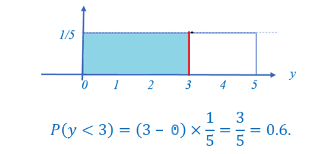
\includegraphics[width=0.5\linewidth]{week03/uniformExample02-1} \end{center}

2).

\begin{center}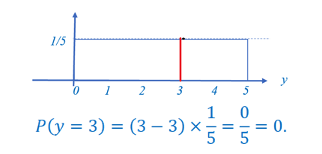
\includegraphics[width=0.5\linewidth]{week03/uniformExample02-2} \end{center}

3).

\begin{center}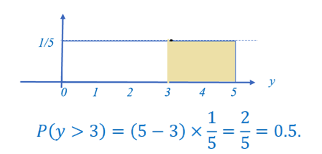
\includegraphics[width=0.5\linewidth]{week03/uniformExample02-3} \end{center}

\hypertarget{normal-distributions}{%
\chapter{Normal Distributions}\label{normal-distributions}}

The standard normal distribution is the most frequently used distribution in this course. We will introduce the general normal distributions and focus on two basic questions: Finding probabilities and percentiles using the standard normal table.

\hfill\break

\hypertarget{standard-normal-distribution}{%
\section{Standard Normal Distribution}\label{standard-normal-distribution}}

The standard normal distribution, \(Z\), has a mean of \(\mu = 0\) and a standard deviation of \(\sigma = 1\). Its probability density curve is

\begin{center}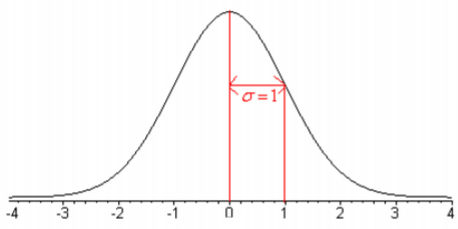
\includegraphics[width=0.6\linewidth]{week04/z-Dist} \end{center}

Two basic types of questions need to be answered for any distribution including the standard normal distribution:

\begin{enumerate}
\def\labelenumi{\arabic{enumi}.}
\item
  Finding probability of events such as P(Z \textless{} a), P(Z \textgreater{} c), P( a \textless{} Z \textless{} b), etc.
\item
  Finding percentiles. For example, finding \(z_0\) for given P(Z \textless{} \(z_0\)) = 0.90.
\end{enumerate}

We have discussed how to find probabilities from the uniform distribution in topic \#3 whose density curve is a rectangle. The probabilities of events defined based on uniform distributions are the areas of rectangles using the area formula of a rectangle. We still need to find the probability of events defined based on the standard normal distribution like P(\(-0.86 < Z < 0\)) which is still the area of the following shaded region (as outlined in the previous note for any general distribution).

\begin{center}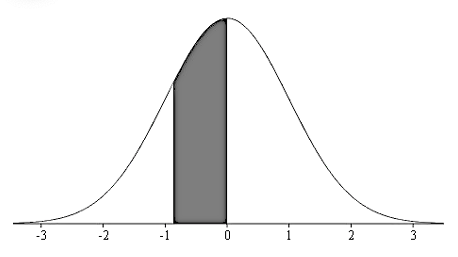
\includegraphics[width=0.6\linewidth]{week04/z-Prob} \end{center}

\hfill\break

\hypertarget{finding-probabilities}{%
\subsection{Finding Probabilities}\label{finding-probabilities}}

Unlike uniform distributions whose density curves are rectangles, we can use the formula to calculate the areas of rectangles. In a standard normal distribution, there is no formula to calculate the area of the shaded irregular region in the above figure.

We will use a standard normal distribution table to find the area of the left-hand side tail regions shown below (part of the table).

\begin{center}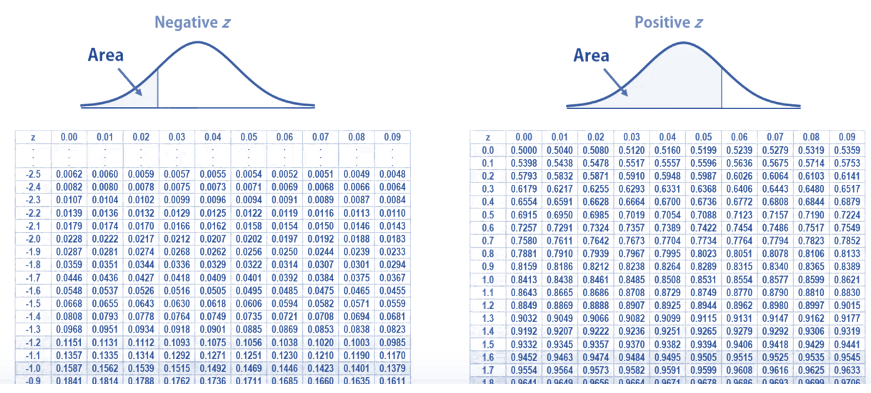
\includegraphics[width=0.6\linewidth]{week04/z-LeftTailArea} \end{center}

Before doing examples, we point out the basic facts of the standard normal distribution.

\begin{enumerate}
\def\labelenumi{\arabic{enumi}.}
\item
  The density curve is symmetric concerning the vertical axis.
\item
  The area between the curve and the horizontal axis is equal to 1. This means that the areas of the left and right regions are equal to 0.5.
\end{enumerate}

Next, we use several examples to illustrate how to use the standard normal table to find the areas of different regions defined based on the standard normal distribution.

Example 1. Find the probabilities indicated, where as always Z denotes a standard normal random variable.

1). P(Z \textless{} - 1.48).

2). P(Z \textless{} 0.25).

\textbf{Solution}. First of all, we only keep two decimal places for the z value (also called z-score). When using the table, we first locate the integral part and the first decimal place of the z score in the \textbf{first column} and the second decimal place in the \textbf{top row}. The \textbf{left tail area} is on the interaction of the aforementioned row and column. This is explained in the following figure.

\begin{center}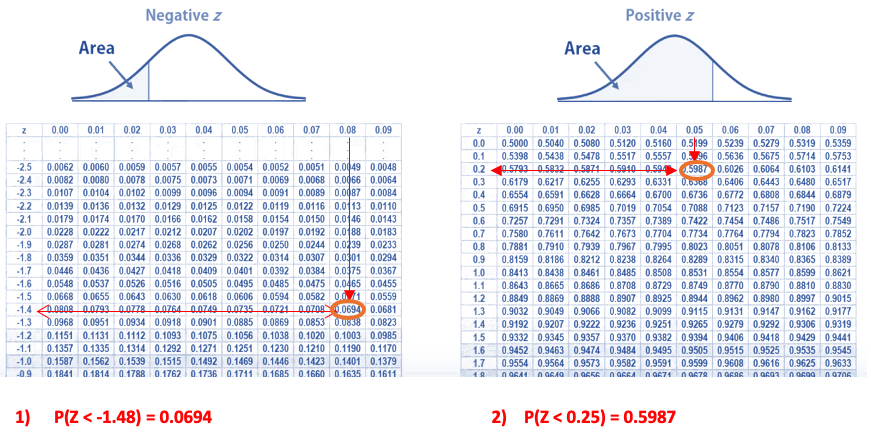
\includegraphics[width=0.6\linewidth]{week04/example01} \end{center}

Example 2. Find the probabilities indicated, where as always Z denotes a standard normal random variable.

1). P(Z \textgreater{} - 1.96).

2). P(Z \textgreater{} 0.75).

\textbf{Solution}: The probabilities to be found represent the areas of right tail regions. We can use the table to find the area of the left tail region and then subtract it from 1 to get the desired probability. The following figure illustrates the idea to get the ``right-tail'' probabilities.

\begin{center}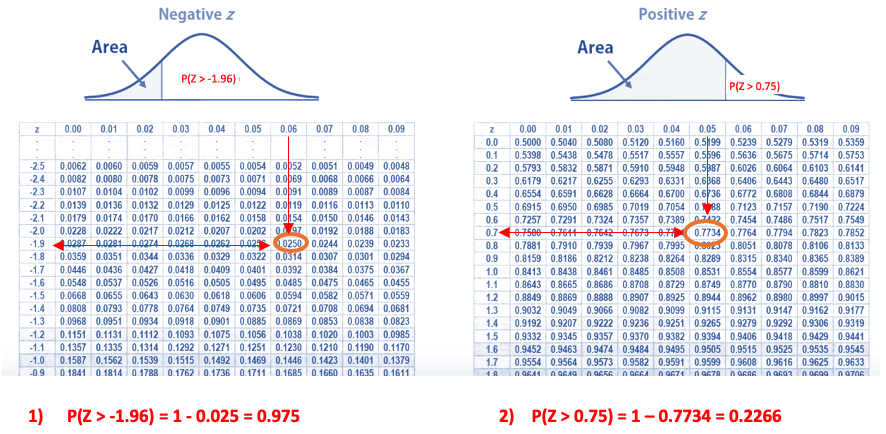
\includegraphics[width=0.6\linewidth]{week04/example02} \end{center}

Example 3. Find the probabilities indicated, where as always Z denotes a standard normal random variable.

1). P(-1.96 \textless{} Z \textless{} 0.75).

\textbf{Solution}: The general idea is to find the two \textbf{left tail areas} and then take the difference to get the area of the region defined by the two z-scores as shown in the following figure.

\begin{center}\includegraphics[width=0.6\linewidth]{week04/betweenArea} \end{center}

For 1), the probability is found in the following figure.

\begin{center}\includegraphics[width=0.6\linewidth]{week04/example03} \end{center}

\textbf{Summary of Finding Probabilities}

\hfill\break

\begin{center}\includegraphics[width=0.6\linewidth]{week04/summaryFindingProb} \end{center}

\hypertarget{finding-percentiles}{%
\subsection{Finding Percentiles}\label{finding-percentiles}}

We have introduced how to find a percentile from a given data set. We basically do the same thing for the standard normal distribution.

Recall that the q-the percentile is the cut-off value such that 100q\% data values are less than or equal to the cut-off value (q-th percentile). This means, we find a percentile, and the left tail area is always given. The general formulation of the problem is to find the cut-off k that satisfies
\[
P(Z < k) = 0.90,
\]
for a given q (such as 90\%, etc). This is depicted in the following figure.

\begin{center}\includegraphics[width=0.6\linewidth]{week04/findingPercentile} \end{center}

The process of finding a percentile is the opposite of the process of finding probability. If the given left tail probability itself is in the main body of the table, we then locate the row and the column to find the z-score (i.e., the percentile).

In general, the given left tail probability is not in the table but is closest to two values in the main boy of the table. Each of the two closed table values corresponds to a z-score. The average of the two z-scores is defined to be the desired percentile.

Example 4. Find 90th percentile of the standard normal distribution.

\textbf{Solution}: We go to the normal table and find two values in the main body of the table that is closest to 0.9 (see the figure below).

\begin{center}\includegraphics[width=0.6\linewidth]{week04/finding90thPercentile} \end{center}

\hfill\break

Example 5. \textbf{The Precision Scientific Instrument Company} manufactures thermometers that are supposed to give readings of \(0^oC\) at the freezing point of water. Tests on a large sample of these instruments reveal that the freezing point of water is around zero (some thermometers give positive degrees, some thermometers give negative degrees), Assume that the mean reading is \(0^oC\) and the standard deviation of the readings is \(1.00^oC\). Assume further that the readings are normally distributed.

\begin{enumerate}
\def\labelenumi{\arabic{enumi}.}
\item
  Find the probability that, at the freezing point of water, the reading is between \(0^oC\) and \(1.58^oC\).
\item
  Find the probability that the reading is between \(–2.43^oC\) and \(0^oC\).
\item
  Find the probability that the reading is between \(0.5^oC\) and \(2.5^oC\).
\item
  Find the probability that the reading is between \(–1^oC\) and \(–2.5^oC\).
\item
  Find the probability that the reading is between \(–1.5^oC\) and \(1^oC\).
\item
  Find the probability that the reading is exactly \(0^oC\).
\item
  Find the temperature z corresponding to \(P_{95}\), the 95th percentile (95\% of the readings less than z and 5\% of the readings are greater than z).
\item
  Fin the 10th percentile.
\end{enumerate}

\textbf{Solution}: Based on the given information, the thermometer readings follow the standard normal distribution. The standard normal distribution table will be used to answer the above questions. We only do questions 5 (finding probability) and 7 (finding percentile) to work and leave the rest of the questions to you to practice.

5). P( -1.5 \textless{} Z \textless{} 0) = P(Z \textless{} 0) - P(Z \textless{} -1.5) = 0.5 - P(Z \textless{} -1.5) = 0.5 - 0.0668 = 0.4332

\begin{center}\includegraphics[width=0.6\linewidth]{week04/example05-5} \end{center}

7). We want to find \(P_{95}\), or equivalently, to find \(k\) from \(P(Z < k) = 0.95\). We can see from the normal table that 0.9495 and 0.9505 are the two values that are closest to 0.95. The two corresponding z-scores are 1.64 and 1.65. By the convention, the 95th percentile is the average of the two z-scores (see the figure below).

\begin{center}\includegraphics[width=0.6\linewidth]{week04/example05-7} \end{center}

\hfill\break

\hfill\break

\hypertarget{general-normal-distribution}{%
\section{General Normal Distribution}\label{general-normal-distribution}}

\hfill\break

In practice, we rarely have a standard normal distribution. Many real-world problems are associated with general normal distribution. We still need to answer the two basic types of questions: finding probabilities and percentile. The following figure illustrates the two types of questions based on the normal distribution with a mean of 500 (\(\mu = 500\)) and a standard deviation of 100 (\(\sigma = 100\))

\begin{center}\includegraphics[width=0.6\linewidth]{week04/twoTypeQuestions} \end{center}

The question is whether we cannot use the standard normal distribution table to answer the above two types of questions associated with general normal distribution.

We can use z-score transformation to transform general normal distributions to the standard normal distribution to use the table and then transform back the original general normal distribution. The following figure outlines the above idea.

\begin{center}\includegraphics[width=0.6\linewidth]{week04/z-ScoreTranform} \end{center}

\hypertarget{finding-probabilities-1}{%
\subsection{Finding Probabilities}\label{finding-probabilities-1}}

We use the following example to show the steps for finding the left-tail probabilities.

Example 6. Consider the general normal distribution \(N(500, 100)\). Find \(P(X < 600) = ?\)

\textbf{Solution}. The following figure shows the z-score transformation to obtain the answer.

\begin{center}\includegraphics[width=0.6\linewidth]{week04/example06} \end{center}

\hypertarget{finding-percentiles-1}{%
\subsection{Finding Percentiles}\label{finding-percentiles-1}}

We continue to use the previous normal distribution as an example to show how to find a percentile of the general normal distribution.

Example 7. Consider the general normal distribution \(N(500, 100)\). Find the 15th percentile.

\textbf{Solution: } We are given that the left tail area is 0.15. After z-score transformation, the left tail area of the standard normal density curve is also 0.15 (see the following figure). We can find \(Z_0\) from \(P(Z < Z_0) = 0.15\) using the standard normal table which is \(Z_0 \approx -1.04\).

\begin{center}\includegraphics[width=0.6\linewidth]{week04/example07} \end{center}

Using the relationship between \(Z_0\) and \(K\) in the z-score transformation (see the above figure). We have

\[
-1.04 = \frac{K - 500}{100}
\]
Solve for \(K\), we have \(K = 500 - 1.04\times 100 = 396\).

Example 8. Tomkins Associates reports that the mean clear height for a Class A warehouse in the United States is 22 feet. Suppose clear heights are normally distributed and that the standard deviation is 4 feet. A Class A warehouse in the United States is randomly selected

a). What is the probability that the clear height is greater than 17 feet?

b). What is the probability that the clear height is less than 13 feet?

c). What is the probability that the clear height is between 25 and 31 feet?

d). Find the clear height such that 10\% of all clear heights are less than it.

\textbf{Solution} The following figures outline the process of finding the answers to each of the questions.

a). P(X \textgreater{} 17) = P(Z \textgreater{} -5/4) = 1 - P(Z \textless{} -5/4) = 0.8944.

\hfill\break

\begin{center}\includegraphics[width=0.6\linewidth]{week04/example08a} \end{center}

b). P(X \textless{} 13) = P(Z \textless{} 9/4) = 0.012.

\hfill\break

\begin{center}\includegraphics[width=0.6\linewidth]{week04/example08b} \end{center}

c). P(25 \textless{} X 31) = P(3/4 \textless{} Z \textless{} 9/4) = P(Z \textless{} 9/4) - P(Z \textless{} 3/4) = 0.9878 - 0.9734 = 0.2144.

\hfill\break

\begin{center}\includegraphics[width=0.6\linewidth]{week04/example08c} \end{center}

d). Since P(Z \textless{} Zo) =0.10, we have Zo = - 1.28 (from the normal table). The desired clear height (10th percentile) is \(X = 22-1.28\times4\) = 16.88 feet.

\hfill\break

\begin{center}\includegraphics[width=0.6\linewidth]{week04/example08d} \end{center}

Example 9. In redesigning jet ejection seats to better accommodate women as pilots, it is found that women's weights are normally distributed with a mean of 143 lb and a standard deviation of 29 lb.

a). If a woman is randomly selected, what is the probability that she weighs between 163 lb and 201 lb?

b). If the current ejection seat for men weighs between 130 lb and 211 lb, what percentage of women have weights that are within those limits?

c). If a woman is randomly selected, what is the probability that she weighs less than 125 lb?

d). If a woman is randomly selected, what is the probability that she weighs exactly 143 lb?

e). If a woman is randomly selected, what is the probability that she weighs between 90 lb and 130 lb?

f). Find the 10th percentile P10, that is, the weight separating the bottom 10\% from the top 90\%.

\textbf{Solution} The following are brief solutions with graphical explanations.

a). P(163 \textless{} X \textless{} 201) = P(0.69 \textless{} Z \textless{} 2) = P(Z \textless{} 2) - P(Z \textless{} 0.69) = 0.9772 - 0.7549 = 0.2223.\\

\begin{center}\includegraphics[width=0.6\linewidth]{week04/example09a} \end{center}

b). P(130 \textless{} X \textless{} 211) = P(-0.45 \textless{} Z \textless{} 2.35) = P(Z \textless{} 2.35) - P(Z \textless{} -0.45) = 0.9906 - 0.3264 = 0.6642.\\

\begin{center}\includegraphics[width=0.6\linewidth]{week04/example09b} \end{center}

c). P(X \textless{} 125) = P(Z \textless{} -0.62) = 0.2676.\\

\begin{center}\includegraphics[width=0.6\linewidth]{week04/example09c} \end{center}

d). P(x=143) = 0.

e). P(90 \textless{} X \textless{} 130) = P(-1.83 \textless{} Z \textless{} -0.45) = P(Z \textless{} -0.45) - P(Z \textless{} -1.83) = 0.3264 - 0.0336 = 0.2928.

\hfill\break

\begin{center}\includegraphics[width=0.6\linewidth]{week04/example09e} \end{center}

f). P(z \textless{} \(z_0\)) = 0.1, so we get \(z_0\) = -1.285. The \(P_{10}\) is calculated by \(x = 143-1.285\times 29 = 105.73\).

\hfill\break

\begin{center}\includegraphics[width=0.6\linewidth]{week04/example09f} \end{center}

\hypertarget{use-of-technology-2}{%
\section{Use of Technology}\label{use-of-technology-2}}

Two of the \textbf{ISLA} apps can be used to answer questions associated with the topics in this chapter. distribution we can use.

\begin{itemize}
\tightlist
\item
  \href{https://wcupeng.shinyapps.io/ZTable/}{Normal Table App} illustrate how to use standard normal table to answer the two basic questions based on the standard normal distribution.
\end{itemize}

\begin{center}\includegraphics[width=0.8\linewidth]{week04/introStatsApps-Ztable} \end{center}

\begin{itemize}
\tightlist
\item
  \href{https://peng-isla.shinyapps.io/TwoQ4NormalDist/}{Genaral Normal Distribution App} can be used to answer the two basic types of questions based on any normal distributions (including the standard normal distribution)
\end{itemize}

\hypertarget{clt-and-sampling-distributions}{%
\chapter{CLT and Sampling Distributions}\label{clt-and-sampling-distributions}}

We have discussed both standard normal and general normal distributions as well as associated two types of questions. In this course, we primarily focus on the inference about the population mean means and proportions from random samples. We will use the sample mean and sample proportion (\texttt{both\ are\ statistics}) to approximate the population mean and proportion (\texttt{both\ are\ parameters}).

Since both sample mean and proportions are statistics, they are random. We need to discuss the distributions of sample means and sample proportions.

\textbf{Some Terminologies}: We have learned concepts of the population (parameters) and sample (statistics) as well as probability distributions of random variables.

\begin{itemize}
\item
  \textbf{Random Sample} is a subset of values that represents the population of interest.
\item
  \textbf{Sampling Distribution} - the distributions of sample statistics are called sampling distributions.
\item
  \textbf{Sampling Distribution of Sample Means} -- A theoretical probability distribution of sample means that would be obtained by drawing from the population all possible samples of the same size.
\item
  \textbf{The Standard Error Sample Mean} -- The standard deviation of the sampling distribution of the mean. It describes how much dispersion there is in the sampling distribution of the mean
\end{itemize}

\hypertarget{central-limit-theorem-clt}{%
\section{Central Limit Theorem (CLT)}\label{central-limit-theorem-clt}}

\begin{quote}
\textbf{Central Limit Theorem}: If all possible random samples of size n are drawn from a population with a mean \(\mu\) and standard deviation \(\sigma\), then as n increases, the sampling distribution of sample means approaches a normal distribution with mean \(\mu\) and standard deviation \(\sigma/\sqrt{n}\).
\end{quote}

\textbf{Remarks}

\begin{enumerate}
\def\labelenumi{\arabic{enumi}.}
\item
  The population distribution is NOT specified in CLT. This implies that the CLT could be used for any population (continuous or discrete).
\item
  The sample size should be large to guarantee a good approximation of the sample mean to a normal distribution. \textbf{How large is large?} \texttt{By\ convention,\ in\ this\ course,\ if\ n\ \textgreater{}\ 30,\ the\ sample\ is\ called\ "large"}.
\item
  The distribution of the sample is \textbf{approximately normally distributed}. The mean of the sample means (\(\bar{X}\)) is equal to the population mean (\(\mu\)) and the standard deviation of the sample mean is equal to \(\sigma/\sqrt{n}\).
\end{enumerate}

In summary, let \(\{X_1, X_2, \cdots, X_n \}\) be a sample taken from a population \((\mu, \sigma)\), by convention, if \(n > 30\),

\[
\bar{X} \to N \big(\mu, \frac{\sigma}{\sqrt{n}} \big)
\]
or equivalently,
\[
\frac{\bar{X}-\mu}{\sigma/\sqrt{n}} \to N(0, 1)
\]

The following figure shows how the sample size impacts the variance of the sample mean.

\begin{center}\includegraphics[width=0.6\linewidth]{week05/CLT} \end{center}

\hfill\break

\textbf{An Important Fact}

\emph{If the population is normal, then}
\[
\bar{X} \to N \big(\mu, \frac{\sigma}{\sqrt{n}} \big)
\]
\emph{regardless of the sample size}.

\hfill\break

Example 1. The length of time people spend driving each day is different in different age groups. A previous study shows that drivers aged 15 to 19 drive on average \(\mu =\) 25 minutes a day and standard deviation \(\sigma =\) 1.5 minutes. A random sample of 50 drivers was selected What is the probability that the average time they spend driving each day is between 24.7 and 25.5 minutes?

\textbf{Solution:} Since \(n = 50 > 30\), from the Central Limit Theorem, the sampling distribution of sample means is approximately normal with \((\mu, \sigma/\sqrt{n}) = (25, 0.21)\).

\begin{center}\includegraphics[width=1\linewidth]{week05/example01} \end{center}

\hfill\break

Example 2. A bank auditor claims that \textbf{credit card balances are normally distributed}, with a mean of \$2870 and a standard deviation of \$900.

\begin{enumerate}
\def\labelenumi{\arabic{enumi}.}
\tightlist
\item
  What is the probability that a randomly selected credit card holder has a credit card balance of less than \$2500?
\end{enumerate}

\textbf{Solution}: Since the card balances are normally distributed, we convert the general normal distribution to the standard normal distribution to find the probability (see the following figure)

\begin{center}\includegraphics[width=1\linewidth]{week05/example02-1} \end{center}

Therefore, there is a 34\% chance that an individual will have a balance of less than \$2500.

\hfill\break

\begin{enumerate}
\def\labelenumi{\arabic{enumi}.}
\setcounter{enumi}{1}
\tightlist
\item
  You randomly select 25 credit cardholders. What is the probability that their mean credit card balance is less than \$2500?
\end{enumerate}

\textbf{Solution}: Because the population is normal, we use the important fact that the sample mean \(\bar{X}\) is normally distributed.

\begin{center}\includegraphics[width=1\linewidth]{week05/example02-2} \end{center}

Therefore, there is only a 2\% chance that the mean of a sample of 25 will have a balance of less than \$2500 (an unusual event).

\begin{enumerate}
\def\labelenumi{\arabic{enumi}.}
\setcounter{enumi}{2}
\tightlist
\item
  Is it possible that the auditor's claim that the mean is exactly \$2870 is incorrect?
\end{enumerate}

\textbf{Solution}

It is impossible since the probability of observing a single value from the population is always zero.

\hfill\break

\hypertarget{sampling-distribution-of-sample-proportion-hatp}{%
\section{\texorpdfstring{Sampling Distribution of Sample Proportion \(\hat{p}\)}{Sampling Distribution of Sample Proportion \textbackslash hat\{p\}}}\label{sampling-distribution-of-sample-proportion-hatp}}

As an application of the central limit theorem, we now discuss the sampling distribution of sample proportion (\(\hat{p}\)).

\begin{itemize}
\item
  In real-world problems, the responses of interest produce counts rather than measurements -- gender (male, female), political preference (republican, democrat), and approval of the new proposal (yes, no).
\item
  Our data will consist of counts or proportions based on the counts.
\item
  We want to learn about population proportions based on the information provided from sample proportions.
\end{itemize}

\textbf{A binary population}: contains only two possible distinct values, say ``success'' and ``failure''.

\textbf{Count}: X = the number of successes in a sample of size n

\textbf{Proportion}: \(\hat{p} =\) the proportion of successes in a sample of size n

\textbf{Sampling Distribution Of A Proportion}: if \(np > 5\) and \(n(1-p) > 5\), then
\[
\hat{p} \to N\Big( p, \sqrt{\frac{p(1-p)}{n}}\Big)
\]
or equivalently

\[
\frac{\hat{p}-p}{\sqrt{\frac{p(1-p)}{n}}} \to N(0, 1)
\]
\textbf{A cautionary note about proportion}: \emph{Whenever working with proportion, we MUST use proportion in the form of decimal in all calculations.}

\hfill\break

Example 3. Suppose it is known that 43\% of Americans own an iPhone. If a random sample of 50 Americans were surveyed, what is the probability that the proportion of the sample who owned an iPhone is between 45\% and 50\%?

\textbf{Solution}: We are given that \(n = 50\) and \(p = 0.43\). Because \(np = 50\times 0.43 = 21.5 > 5\) and \(n(1-p) = 50 \times (1-0.43) = 28.5 > 5\), we use the above sampling distribution. The following figure gives the steps for finding the probability.

\begin{center}\includegraphics[width=1\linewidth]{week05/example03} \end{center}

\hfill\break

\hypertarget{use-of-technology-3}{%
\section{Use of Technology}\label{use-of-technology-3}}

Three \textbf{IntroStatsApps} were created to illustrate the central limit theorem (CLT) and its applications. The solutions of the above examples were produced using ** IntroStatsApps**.

\hypertarget{clt-demo}{%
\subsection{CLT Demo}\label{clt-demo}}

\textbf{IntroStatsApps-Central Limit Theorem Demo} illustrates the CLT with various populations including the normal population. You can click the link (\url{https://wcupeng.shinyapps.io/CLTdemo/}) to explore the CLT under different populations. See the following screenshot of the demo.

\begin{center}\includegraphics[width=1\linewidth]{week05/cltDemo} \end{center}

\hypertarget{clt-for-mean}{%
\subsection{CLT for Mean}\label{clt-for-mean}}

When the sampling distribution is normal (the cases of CLT or normal population), we can use this application to answer questions of probability and percentile. The link to this application is at: \url{https://wcupeng.shinyapps.io/AppsCLT4Means/}.

\begin{center}\includegraphics[width=1\linewidth]{week05/cltMean} \end{center}

\hypertarget{clt-for-proportion}{%
\subsection{CLT for Proportion}\label{clt-for-proportion}}

For the sampling distribution of sample proportion, we use the following application to answer the questions about probability and percentile. The link to the applications is at: \url{https://wcupeng.shinyapps.io/AppsCLT4Prop/}.

\begin{center}\includegraphics[width=1\linewidth]{week05/cltProp} \end{center}

\hfill\break

\hypertarget{practice-exercises}{%
\section{Practice Exercises}\label{practice-exercises}}

\begin{enumerate}
\def\labelenumi{\arabic{enumi}.}
\item
  The U.S. National Center for Health Statistics publishes information on the length of stay by patients in short-stay hospitals in Vital and Health Statistics. According to that publication, the mean stay of female patients in short-stay hospitals is 5.8 days and the standard deviation is 4.3 days. Let \(\bar{x}\) denote the mean length of stay for a sample of discharged female patients.

  A). For a sample size of 81, find the mean and standard deviation of the sample mean. Interpret your results in words.

  B). Repeat part A) with n = 144. Find the percentage that the mean stay of those 144 female patients in short-stay hospitals is less than 5 days.
\end{enumerate}

\hfill\break

\begin{enumerate}
\def\labelenumi{\arabic{enumi}.}
\setcounter{enumi}{1}
\item
  According to the U.S. Census Bureau publication Current Construction Reports, the mean price of new mobile homes is \$43,800. The standard deviation of the prices is \$7200. Let \(\bar{x}\) denote the mean price of a sample of new mobile homes.

  A). For a sample of 49 randomly selected mobile homes, find the mean and standard deviation of the sample mean.

  B). Repeat part A) with n =100. Compare the results you obtained in A).

  C ). For a sample of 64 randomly selected mobile homes, find the probability that the mean is greater than \$45,000.

  D). For a sample of 64 randomly selected mobile homes, find the probability that the mean is exactly \$45,000.
\end{enumerate}

\hfill\break

\begin{enumerate}
\def\labelenumi{\arabic{enumi}.}
\setcounter{enumi}{2}
\item
  Suppose that the ages \(X\) of a certain population are normally distributed, with mean \(\mu = 27.0\) years, and standard deviation \(\sigma = 12.0\) years, i.e., \(X \to N(27,12)\).

  Find the probability that the mean age of a single sample of \(n = 16\) randomly selected individuals is less than 30 years.
\end{enumerate}

\hfill\break

\begin{enumerate}
\def\labelenumi{\arabic{enumi}.}
\setcounter{enumi}{3}
\tightlist
\item
  Fifty-one percent of adults in the U.S. whose New Year resolved to exercise more achieved their resolution. You randomly select 65 adults in the U.S. whose resolution was to exercise more and ask each if he or she achieved that resolution. What is the probability that the sample proportion is greater than 50\%?
\end{enumerate}

\hypertarget{confidence-intervals-for-population-means}{%
\chapter{Confidence Intervals for Population Means}\label{confidence-intervals-for-population-means}}

We will discuss the general framework of confidence intervals of population means and proportions. In the next few sections, we learn how to \textbf{estimate the population parameters} such as mean, standard deviation, and proportion from a random sample and build a confidence interval (also called interval estimate) to show how good the estimate is, and finally, we should be able to interpret the estimate.

\hypertarget{a-general-framework}{%
\section{A General Framework}\label{a-general-framework}}

This section dedicates the basic framework to estimating population means using confidence intervals.

\hypertarget{some-technical-terms}{%
\subsection{Some Technical Terms}\label{some-technical-terms}}

The following is a list of several basic terms to use when discussing the estimate of population parameters.

\begin{itemize}
\item
  An \textbf{estimate} is \emph{a specific value} or \emph{range of values} obtained from a random sample that is used to approximate a population parameter.
\item
  A \textbf{point estimate} is a single value (obtained from the random sample) that is used to approximate a population parameter.
\end{itemize}

Example 1. The sample mean, denoted by \(\bar{x}\), is the best point estimate of the population mean \(\mu\).

Example 2. The sample variance, denoted by \(s^2\) is the best point estimate of the population variance \(\sigma^2\).

\begin{itemize}
\item
  The \textbf{bias of the point estimate} is equal to the difference between the estimate and the true parameter. For example, the bias of the sample mean is \(\bar{x} -\mu\). The bias of an estimate measures \emph{the accuracy of the estimate}.
\item
  Since the point estimate of a parameter is obtained from an underlying random sample, it is a random variable. The variance of the point estimate measures the precision of the point estimate of the corresponding population parameter.
\item
  \textbf{The goodness of an estimate} -- \emph{no bias and small variance}.
\end{itemize}

\hfill\break

\hypertarget{issues-of-a-point-estimate-and-the-logic-for-developing-a-solution}{%
\subsection{Issues of A Point Estimate and the Logic for Developing A Solution}\label{issues-of-a-point-estimate-and-the-logic-for-developing-a-solution}}

For a point estimate, we can only say that it is close to the true population parameter. Three questions remain to answer:

1). How close is ``close''?

2). How confident is your statement?

3). How precise is the estimate?

We use the following artificial example to explain the above issues about a \textbf{point estimate} of the population mean.

Example 3. Assume that the true mean height of WCU student population is 69 inches. To estimate the true mean, we randomly select a sample of 50 students and measure their heights to get a random sample of 50 heights. Assume that the sample average of 68.5 inches.

Now the question: \textbf{Is 68.5 close to 69? }

Apparently, we cannot provide an objective answer to the above question with a single sample mean without any additional information.

To address the issue, let's pretend sampling is free. We could take as many samples of the same size using the same protocol as we wish. Then we get many sample means. For example, pretending we obtained 100 sample means from 100 random samples taken from the WCU student population with the same size of 50.

\begin{verbatim}
68.2 68.3 68.3 68.4 68.4 68.5 68.6 68.6 68.6 68.6 68.6 68.7 68.7 68.7 68.7 68.7 
68.7 68.7 68.8 68.8 68.8 68.8 68.8 68.8 68.8 68.8 68.8 68.8 68.8 68.8 68.8 68.8 
68.9 68.9 68.9 68.9 68.9 68.9 68.9 68.9 68.9 68.9 68.9 68.9 69.0 69.0 69.0 69.0
69.0 69.0 69.0 69.0 69.0 69.0 69.0 69.1 69.1 69.1 69.1 69.1 69.1 69.1 69.1 69.1 
69.1 69.1 69.1 69.2 69.2 69.2 69.2 69.2 69.2 69.2 69.2 69.2 69.2 69.3 69.3 69.3 
69.3 69.3 69.3 69.4 69.4 69.4 69.5 69.5 69.5 69.5 69.5 69.5 69.6 69.6 69.6 69.6
69.7 69.7 69.7 69.9
\end{verbatim}

With these sample means, we make a histogram in the following

\begin{center}\includegraphics[width=0.6\linewidth]{week06/example03} \end{center}

We use the definition of percentile to find 2.5\% and 97.5\% percentiles to be 68.3, and 69.7 respectively (shown in the above figure). This means that 95\% of the sample means are within interval: {[}68.3, 69.7{]}. Clearly, 69 is inside the interval.

With the above interval, address the aforementioned three issues:

\begin{itemize}
\item
  \textbf{All values inside the interval are considered to be close to the true mean of 69.}
\item
  The interval contains 95\% of the sample means. If a sample mean is in the interval, we are 95\% confident that the sample mean is close to the true mean of 69.
\item
  The width of the interval (\(69.7 - 68.3 = 1.4\)) reflects the precision of the estimate.
\end{itemize}

Therefore, this interval contains all desired information, but what is more important is that \textbf{the interval was constructed from the distribution of sample means}.

\textbf{Definition 1: } The area of \(0.95 = 95\%\) of the middle region in the above figure is called ** 95\% Confidence Level**.

\textbf{Definition 2: } \emph{The above interval is called the 95\% confidence interval of the average height of WCU student population}. Furthermore, \textbf{68.3} is called lower confidence limit (LCL) and \textbf{69.7} is called upper confidence limit (UCL).

The above interval was found based on the histogram of 100 sample means. In real-world applications, taking multiple samples could be very costly. \textbf{The new and practical question is} \emph{how to find an interval similar to the above one without taking multiple samples}.

\hfill\break

\hypertarget{general-framework-of-confidence-intervals}{%
\subsection{General Framework of Confidence Intervals}\label{general-framework-of-confidence-intervals}}

The key information needed to find the confidence interval of a population mean (\(\mu\)) is to know the distribution of the sample mean (\(\bar{X}\)). The distribution of \(\bar{X}\) is also called the sampling distribution of the sample mean.

We have discussed the sampling distribution of sample \(\bar{X}\) in the previous note.

\begin{itemize}
\tightlist
\item
  If the sample size \(n > 30\), by the CLT, the distribution of the sample mean (\(\bar{X}\)) is \emph{approximately} normal with the mean and standard deviation specified below
\end{itemize}

\[
\bar{X} \to N\Big( \mu, \frac{\sigma}{\sqrt{n}} \Big)
\]

\begin{itemize}
\tightlist
\item
  If the population is normally distributed as \(N(\mu, \sigma)\), the
\end{itemize}

\[
\bar{X} \to N\Big( \mu, \frac{\sigma}{\sqrt{n}} \Big)
\]

regardless of the sample size.

\begin{itemize}
\tightlist
\item
  For a binary population with success probability \(p\), the sampling distribution of sample proportion (\(\hat{p}\)) is
\end{itemize}

\[
\hat{p} \to N\Big(p, \sqrt{\frac{p(1-p)}{n}} \Big)
\]

\hfill\break
\textbf{Thought Process of Obtaining A Confidence Interval of Population Mean}\\

With the above sampling distribution, we can find the confidence interval without taking multiple samples. Next, we use the sampling distribution based on the CLT to illustrate the logic for obtaining the confidence interval of the population mean (\(\mu\)).

\begin{itemize}
\tightlist
\item
  when \(n > 30\),
\end{itemize}

\[
\bar{X} \to N\Big(\mu, \frac{\sigma}{\sqrt{n}}\Big)
\]

\begin{center}\includegraphics[width=0.6\linewidth]{week06/samplingConfLimits} \end{center}

For the given \texttt{95\%\ confidence\ level} (the area of the middle region in the above figure), we cannot find the \texttt{confidence\ limits\ LCL\ and\ UCL} directly from the normal table since \(\bar{X}\).

\begin{itemize}
\tightlist
\item
  However, we can use z-score transformation to transform the sampling distribution of \(\bar{X}\) to the standard normal distribution in the following.
  \[
  Z = \frac{\bar{X}-\mu}{\sigma/\sqrt{n}} \to N(0, 1)
  \]
\end{itemize}

\begin{center}\includegraphics[width=0.6\linewidth]{week06/stdNormConfLimits} \end{center}

When the area of the middle region in the above standard normal curve is given to be 0.95, we can find the 2.5\% and 97.5\% percentiles (-1.96 and 1.96 respectively) from the normal table directly.

\textbf{Definition 3: } The percentiles \(\pm 1.96\) are called \textbf{critical values (CV)} of 95\% confidence level for the standard normal distribution. The two critical values are symmetric to the origin!

\hfill\break

\begin{itemize}
\tightlist
\item
  Relationship between Critical Values and Confidence Limits
\end{itemize}

The critical values corresponding to the 95\% confidence level are \(\pm 1.96\). Using the z-score transformation, we have the following relationship.
\[
-1.96 = \frac{LCL - \mu}{\sigma/\sqrt{n}}
\]
and
\[
1.96 = \frac{UCL - \mu}{\sigma/\sqrt{n}}
\]
We can solve the confidence limits

\[
LCL = \mu - 1.96\times \frac{\sigma}{\sqrt{n}}, \ \ \ \ \  UCL =  \mu + 1.96\times \frac{\sigma}{\sqrt{n}}
\]

\begin{itemize}
\tightlist
\item
  If we replace \(\mu\) and \(\sigma\) with sample mean \(\bar{X}\) and sample standard deviation \(s\), then LCL and UCL will be completely dependent on the sample data. Then 95\% confidence interval can be written as
\end{itemize}

\[
(LCL, UCL) = (\bar{X} - 1.96\times \frac{s}{\sqrt{n}}, \ \ \ \ \ \bar{X} + 1.96\times \frac{s}{\sqrt{n}})
\]

\begin{itemize}
\tightlist
\item
  Since the confidence interval is constructed based on the random sample, it is random. We can interpret the confidence interval: \textbf{there is a 95\% chance that the confidence interval {[}68.3, 69.7{]} contains the true population mean (\(\mu\)).}
\end{itemize}

\hfill\break
The above thought process is summarized in the following chart

\begin{center}\includegraphics[width=0.8\linewidth]{week06/summaryCIProcess} \end{center}

\hfill\break

Example 4. Suppose we want to estimate, with 95\% confidence level, the mean (average) length of all walleye fingerlings in a fish hatchery pond. A random sample of 100 fingerlings was selected. The average length is 7.5 inches and the standard deviation is 2.3 inches. That is, \(\bar{x} = 7.5\), \(s = 2.3\), and \(n = 100\).

\textbf{Solution}: Since \(n = 100 > 30\), by the central limit theorem, the sample mean is approximately distributed. The 95\% critical values are \(\pm 1.96\) (using normal table). Based on the above discussion, the lower and upper confidence limits are
\[
(LCL, UCL) = (7.5 - 1.96\times 2.3/\sqrt{100}, \ \ 7.5 + 1.96\times 2.3/\sqrt{100}) = (7.05, \ 7.95)
\]
That is, interval \((7.05, \ 7.95)\) has a 95\% chance of containing the true population mean length of all walleye fingerlings in a fish hatchery pond.

\hfill\break

\hypertarget{formal-steps-for-constructing-c.i.}{%
\section{Formal Steps For Constructing C.I.}\label{formal-steps-for-constructing-c.i.}}

We now formulate the steps for constructing a CI based on the above framework and introduce a few new concepts.

\textbf{Step 1}: Identify the confidence level. If it is NOT given, our default confidence level \(1 - \alpha = 0.95\) should be used in this class.

\textbf{Step 2}: Based on the confidence level to find the critical value from the normal table.

\textbf{Step 3}: Evaluate the margin of error, denoted by E and defined to be
\[
E = CV \times \frac{s}{\sqrt{n}}
\]
\textbf{Step 4}: Write out the confidence interval explicitly in the following form
\[
\bar{x} \pm E = (\bar{x} - E, \ \bar{x} + E)
\]

\textbf{Step 5}: Interpretation of the confidence interval: Two versions of interpretations

\begin{verbatim}
Version #1: We are 95% confident that the interval contains the population mean

Version #2: There is a 95% chance that the interval contains the population means.
\end{verbatim}

\hfill\break

\textbf{Some Remarks}: The following important general facts of confidence intervals can be visualized using \textbf{IntroStatsApps: Normal Confidence Interval} at: \url{https://wcu-peng.shinyapps.io/NormalCI4MeanProp/}

\begin{itemize}
\tightlist
\item
  By convention, we use \(1 - \alpha\) to denote the confidence level (i.e., the area of the middle symmetric region on the density curve). This means that \(\alpha\) is the sum of the two tail areas. In other words, both left and right tail areas are equal to \(\alpha / 2\).
\end{itemize}

\begin{center}\includegraphics[width=0.6\linewidth]{week06/confLevel} \end{center}

\begin{itemize}
\item
  The margin of error, E, is equal to half of the width of the interval.
\item
  Since sample size, n, is in the denominator of E, as sample size increases, E decreases. This implies that as the sample size increases, the interval gets narrower (See the following formula).
\end{itemize}

\begin{center}\includegraphics[width=0.6\linewidth]{week06/ciFormula} \end{center}

\begin{itemize}
\tightlist
\item
  As the level of confidence increases, the critical value (CV) increases. This implies that the width of the confidence interval increases as the confidence level increases (see the above formula for this relationship).
\end{itemize}

\hfill\break

\textbf{Example 5.} Assume that we collect 81 measurements of the iron-solution index of tin-plate specimens, designed to measure the corrosion resistance of tin-plated steel. Assume that the sample mean is 57 and the sample standard deviation is 15. Construct a 95\% confidence interval of the iron-solution index.

\textbf{Solution} We will follow the 5-step procedure to construct the confidence interval.

\textbf{Step 1}: The confidence level \(1 - \alpha = 0.95\), this means that \(\alpha/2 = 0.025\).

\textbf{Step 2}: The critical value is \(CV = Z_{0.025} = 1.96.\)

\textbf{Step 3}: The margin of error
\[
E = CV\times \frac{s}{\sqrt{n}} = 1.96\times \frac{15}{\sqrt{81}} = 3.27.
\]

\textbf{Step 4}: The explicit expression of the 95\% CI is given by
\[
57 \pm E = (57 - 3.27, \ 57 + 3.27) = (53.73, \ 60.27).
\]

\textbf{Step 5}: The interpretation of CI.
We are 95\% confident that the interval (53.73, ~60.27) contains the true population mean of the iron-solution index.

\hfill\break

\textbf{Example 6} (continuation of Example 5). If we change the confidence level from 95\% to 90\% and 99\% respectively, how will be the corresponding \textbf{margin of error} and \textbf{confidence interval} changed?

\textbf{Solution}. We follow the first four of the same 5-step procedure to calculate the margin of error and construct the confidence interval corresponding to the three significant levels and summarize the results in the following figure.

\begin{center}\includegraphics[width=0.8\linewidth]{week06/marginEandWidthCI} \end{center}

We can see the same patterns outlined earlier. as the confidence level increases, the margin of error gets bigger (the left panel in the above figure), hence, the corresponding confidence interval gets wider (the right panel of the figure).

\hfill\break

\hfill\break

\hypertarget{use-of-technology-4}{%
\section{Use of Technology}\label{use-of-technology-4}}

I also created an interactive application to generate confidence intervals for population mean and proportion based on the assumption of large samples. The app is at: \url{https://wcu-peng.shinyapps.io/NormalCI4MeanProp/}

\hfill\break

The following is the screenshot of the solution of Example 5 generated by the app.

\hfill\break

\hfill\break

\begin{center}\includegraphics[width=1\linewidth]{week06/ciNormalDemo} \end{center}

\hypertarget{confidence-intervals-for-population-means-and-proportions}{%
\chapter{Confidence Intervals for Population Means and Proportions}\label{confidence-intervals-for-population-means-and-proportions}}

We have developed the steps for constructing confidence intervals for population means based on large samples with which the central limit theorem can be used to find the sampling distribution of the sample mean.

\begin{center}\includegraphics[width=0.6\linewidth]{week07/ciFormulaReCap} \end{center}

As a review, we present the following example to highlight the importance of the steps for constructing a confidence interval.

Example 1. Market researchers use the number of sentences per advertisement as a measure of readability for magazine advertisements. The following represents a random sample of the number of sentences found in 50 advertisements. (Source: Journal of Advertising Research)

\begin{verbatim}
9  20   18  16  9  9  11  13   22  16    5  18   6    6   5   12   25
17  23  7  10   9   10   10    5   11  18   18   9  9   17  13  11  7
14  6   11   12  11   6   12   14  11    9   18  12  12   17  11   20
\end{verbatim}

The summarized statistics are given in the following table.

\begin{center}\includegraphics[width=0.6\linewidth]{week07/example01DataSummary} \end{center}

Based on the above data, construct a 95\% confidence interval of the mean number of sentences (µ) in all magazine advertisements.

\textbf{Solution} We are going to use the 5-step procedure to construct the confidence interval in the following.

\textbf{Step 1}: We are given a confidence level of 95\%.

\textbf{Step 2}: Since the sample size \(n = 50 > 30\), using the CLT, we claim that the sample mean is approximately normally distributed. The critical value based on the standard normal distribution should be used. The critical value was found and labeled in the following figure.

\begin{center}\includegraphics[width=0.6\linewidth]{week07/example01CV} \end{center}

\textbf{Step 3}: Find the margin of error E in the following
\[
E = Z_{\alpha/2}\times \frac{s}{\sqrt{n}} \approx 1.96\times \frac{5.0}{\sqrt{50}} \approx 1.4.
\]

\textbf{Step 4}: The explicit form of the confidence interval is given by
\[
(\bar{X} - E, \ \bar{X} - E) = (12.4 - 1.4, \ 12.4 + 1.4) = (11.0, 13.8).
\]

\textbf{Step 5}: The confidence interval (11,13.8,) has a 95\% chance to include the true average number of sentences in all magazine advertisements.

\hfill\break

\hypertarget{confidence-interval-of-proportion}{%
\section{Confidence Interval of Proportion}\label{confidence-interval-of-proportion}}

Recall that the sample proportion (\(\hat{p}\)) is approximately normally distributed if both \(n\hat{p}\) and \(n(1-\hat{p})\) are large. To be more specific, in this course, if \(n\hat{p} \ge 5\) and \(n(1-\hat{p}) \ge 5\), we have
\[
\hat{p} \to N\Big(p, \sqrt{\frac{p(1-p)}{n}}  \Big),
\]

which is equivalent to

\[
\frac{\hat{p} - p}{\sqrt{\frac{p(1-p)}{n}}} \to N(0, 1).
\]

Therefore, we can use the same 5-step procedure as used previously in constructing the confidence interval of the population mean for the large sample. The only difference is that the form of the margin of error involves the sampling error of the sample proportion. The following annotated formula explains the components of the confidence interval of the proportion.

\begin{center}\includegraphics[width=0.6\linewidth]{week07/ciPropotionFormula} \end{center}

Next, we use an example to illustrate the 5-step procedure for constructing the confidence interval of proportion.

Example 2. In a survey of 1219 U.S. adults, 354 said that their favorite sport to watch is football. Construct a 95\% confidence interval for the proportion of adults in the United States who say that their favorite sport to watch is football.

\textbf{Solution}: First of all, the sample proportion \(\hat{p} = 354/1219 \approx 0.29\) and sample size \(n = 1219\).

\textbf{Step 1}: The confidence level is \(1 - \alpha = 0.95\). \(\alpha/2 = 0.025\).

\textbf{Step 2}: Since \(n\hat{p} = 354 > 5\) and \(n(1-\hat{p}) = 1219 \times 0.71 = 865 > 5\), the sampling distribution of \(\hat{p}\) is normally distributed. The critical value corresponding to 95\% confidence level is \(Z_{0.025} = 1.96\) (from the normal table).

\begin{center}\includegraphics[width=0.6\linewidth]{week07/example01CV} \end{center}

\textbf{Step 3}: The margin of error for the confidence interval of population proportion is given by
\[
E = Z_{\alpha/2}\times\sqrt{\frac{\hat{p}(1-\hat{p})}{n}} = 1.96\times \sqrt{\frac{0.29(1-0.29)}{1219}} \approx 0.025.
\]

\textbf{Step 4}: The explicit form of the confidence interval is given by
\[
(\hat{p} - E, \ \hat{p} + E) = (0.29 - 0.025, \ 0.29 + 0.025) = (0.365, \ 0.315).
\]

\textbf{Step 5}: The confidence interval (0.265, 0.315) has a 95\% chance to include the true proportion of adults who say football is their favorite sport.

\hfill\break

\hypertarget{t---confidence-interval-for-mean-mu}{%
\section{\texorpdfstring{t - Confidence Interval for Mean (\(\mu\))}{t - Confidence Interval for Mean (\textbackslash mu)}}\label{t---confidence-interval-for-mean-mu}}

We have constructed confidence intervals based on the CLT that require a large sample size. When we construct a confidence interval based on small samples, we need to make stronger assumptions about the population so that we have enough information for the interval.

\hypertarget{t-distribution-and-t-table}{%
\subsection{t-distribution and t-Table}\label{t-distribution-and-t-table}}

We have pointed out that
\[
\frac{\bar{X} - \mu}{\sigma/\sqrt{n}} \to N(0, 1)
\]
if the sample is from a normal population regardless of the sample size. However, if the population is unknown, we need to use the sample standard deviation to estimate the population standard deviation. In this case,

\[
\frac{\bar{X} - \mu}{s/\sqrt{n}} \not \rightarrow N(0, 1)
\]
\textbf{if the sample size is small!} The correct distribution is called t-distribution with \(n-1\) degrees of freedom.

The difference between standard normal and t-distributions are depicted in the following figure.

\begin{center}\includegraphics[width=0.8\linewidth]{week07/t-Dist} \end{center}

We can see from the above figure that t-distributions are also bell-shaped. As the degrees of freedom increase, the t-distributions approach the standard normal distribution! \textbf{However}, when the degree of freedom is small, the t-distribution and the standard normal distribution are VERY different.

This implies that when a small sample from a normal population with unknown population variance, we should NOT use the normal critical value to construct the confidence interval for the unknown population mean. Instead, we MUST use the t-critical value that can be found in the t-table!

Example 3. Find the critical value for a 95\% confidence when the sample size is 15.

\textbf{Solution} since sample size \(n = 15\), the degrees of freedom \(df = n -1 = 14.\) We use the notation \(t_{df, \alpha/2}\) to denote the critical value based on the t-distribution. The following figure shows the location of the CV on the density curve.

\begin{center}\includegraphics[width=0.4\linewidth]{week07/t-CV} \end{center}

The critical value \(CV = t_{14, 0.025} = 2.145\) which is found from the t-distribution table. The following table illustrates the structure of the t-table and how to use the t-table to find the critical value.

\begin{center}\includegraphics[width=0.7\linewidth]{week07/t-Table} \end{center}

\hypertarget{t-confidence-interval}{%
\subsection{t-confidence Interval}\label{t-confidence-interval}}

The steps for constructing t-confidence intervals are identical to those in the normal confidence intervals except for the critical value that is found in the t-table. We will use an example to show the steps for constructing a t-confidence interval.

Example 4. . Estimating Car Pollution - In a sample of seven cars, each car was tested for nitrogen-oxide emissions (in grams per mile) and the following results were obtained: \texttt{0.06,\ 0.11,\ 0.16,\ 0.15,\ 0.14,\ 0.08,\ 0.15} (based on data from the Environmental Protection Agency). Assuming that this sample is representative of the cars in use. Further, the amounts of nitrogen-oxide emission for all cars are normally distributed. Construct a 98\% confidence interval estimate of the mean amount of nitrogen-oxide emission for all cars

\textbf{Solution}: We first calculate the sample mean and sample standard deviation using the formulas introduced in the note of descriptive statistics.
\[
\bar{x} = 0.1214, \ \ \ s = 0.0389.
\]

\textbf{Step 1}: The confidence level for the t-confidence interval is \(1-\alpha = 0.98\). The right-tailed area of the t-density curve is \(\alpha/2 = 0.01\)

\textbf{Step 2}: We need to use the t-critical value to calculate the confidence interval: CV = \(t_{6, 0.01} = 3.143\). The density curve and the table below.

\begin{center}\includegraphics[width=0.7\linewidth]{week07/example04CV} \end{center}

\begin{center}\includegraphics[width=0.7\linewidth]{week07/example04Table} \end{center}

\textbf{Step 3}: The margin of error
\[
E = t_{n-1, \alpha/2} \times \frac{s}{\sqrt{n}} = 3.143\times\frac{0.0398}{\sqrt{7}} \approx 0.0462.
\]

\textbf{Step 4}: Therefore, the 98\% confidence interval estimate of the population mean is\\
\((\bar{x} - E, \bar{x} + E)= (0.1214-0.0462, 0.1214+0.0462) = (0.075, 0.168)\).

\textbf{Step 5}: The interval (0.075, 0.168) has a 98\% chance to include the true average amount of nitrogen-oxide emission of all cars in use.

\hypertarget{normal-or-t-confidence-interval-a-summary}{%
\subsection{Normal or t-Confidence Interval: A Summary}\label{normal-or-t-confidence-interval-a-summary}}

When a normal or t confidence interval should be constructed is dependent on the given amount of information. The following brief flow chart summarizes the selection of the two types of confidence intervals based on different conditions.

\begin{center}\includegraphics[width=0.6\linewidth]{week07/normalOrT} \end{center}

\hfill\break

\hypertarget{use-of-technology-5}{%
\section{Use of Technology}\label{use-of-technology-5}}

Two \textbf{IntroStatsApps} can be used to generate solutions to most of the problems. You can these apps to check your work and make sure you correctly understand the concepts and steps for finding the confidence intervals of either population mean or proportion.

\hypertarget{introstatsapps-normal-ci}{%
\subsection{\texorpdfstring{\textbf{IntroStatsApps}: Normal CI}{IntroStatsApps: Normal CI}}\label{introstatsapps-normal-ci}}

The direct link to the app is at: \url{https://wcu-peng.shinyapps.io/NormalCI4MeanProp/}. The following screenshot is the solution to \textbf{Example 1}.

\begin{center}\includegraphics[width=0.8\linewidth]{week07/appsMeanProp} \end{center}

\hypertarget{introstatsapps-t-ci}{%
\subsection{\texorpdfstring{\textbf{IntroStatsApps}: t-CI}{IntroStatsApps: t-CI}}\label{introstatsapps-t-ci}}

The following apps generate solutions for t-confidence intervals. The direct link is at: \url{https://wcu-peng.shinyapps.io/Student-t-CI/}

The following screenshot is the solution to \textbf{Example 4}.

\begin{center}\includegraphics[width=0.9\linewidth]{week07/appsT-CI} \end{center}

\hypertarget{introstatsapps-t-table}{%
\subsection{\texorpdfstring{\textbf{IntroStatsApps}: t-Table}{IntroStatsApps: t-Table}}\label{introstatsapps-t-table}}

For convenience, I also create an interactive t-table that provides the correct probability or percentile based on the provided information. The direct link is at: \url{https://wcu-peng.shinyapps.io/t-Table/}

The following screenshot is the solution to \textbf{Example 3}.

\begin{center}\includegraphics[width=0.9\linewidth]{week07/appsT-Table} \end{center}

\hfill\break

\hfill\break

\hypertarget{practice-exercises-1}{%
\section{Practice Exercises}\label{practice-exercises-1}}

\hfill\break
Please do the following problems manually and then use the \textbf{IntroStatsApps} to check your work.

\hfill\break

\begin{enumerate}
\def\labelenumi{\arabic{enumi}.}
\item
  A team of efficiency experts intends to use the mean of a random sample of size n =150 to estimate the average mechanical aptitude of assembly-line workers in a large industry (as measured by a certain standardized test) and found that the sample mean is 19.9 minutes, and the sample standard deviation is 5.73 minutes. Construct a 95\% confidence interval for the average mechanical aptitude of assembly line workers in the given industry.
\item
  A college admissions director wishes to estimate the mean age of all students currently enrolled. In a random sample of 20 students, the mean age is found to be 22.9 years. From past studies, the standard deviation is known to be 1.5 years, and the population is normally distributed. Construct a 90\% confidence interval of the population mean age.
\item
  Suppose you are interested in investigating the factors that affect the prevalence of tuberculosis among intravenous drug users. In a group of 97 individuals who admit to sharing needles, 24.7\% had a positive tuberculin skin test result. Construct 95\% confidence intervals for the population proportions.
\item
  Find the confidence interval for average SAT score for women given that n =15, the sample mean is 496, and the sample standard deviation is 108. Assume that the SAT scores are normally distributed.
\end{enumerate}

\hypertarget{the-logic-and-components-of-hypothesis-testing}{%
\chapter{The Logic and Components of Hypothesis Testing}\label{the-logic-and-components-of-hypothesis-testing}}

We have introduced how to construct confidence intervals to estimate the population means and proportion under various assumptions. We now introduce a new inference that justifies a statement about a population mean or proportion - \textbf{Testing Hypotheses}.

\begin{itemize}
\item
  In statistics, a hypothesis is a claim or statement about a property of a population. A hypothesis test is a process that uses sample statistics to test a claim about the value of a population parameter.
\item
  The fundamental idea is to let data speak truthfully.
\item
  \textbf{Rare Event Rule for Inferential Statistics}

  Under a given assumption (e.g., the null hypothesis is correct), if the probability of an observed event is exceptionally small, we conclude that the assumption (the null hypothesis) is probably not correct.
\end{itemize}

Example 1. If someone claims that the average height of WCU student population is at least 80 inches. To justify the claim, we take a random sample of 100 students (a set of representatives of the WCU student population). Assume that the sample mean is 68 inches and the standard deviation 15 inches.

\hfill\break

\hypertarget{steps-for-hypothesis-testing-some-analogies}{%
\section{Steps for Hypothesis Testing: Some Analogies}\label{steps-for-hypothesis-testing-some-analogies}}

To better understand the logic and steps for conducting a statistical hypothesis and the types of inevitable errors in the decision process, we use the two analogies that are familiar to us.

\begin{center}\includegraphics[width=1\linewidth]{week08/analogyHT} \end{center}

No matter what decision will be made, there are two possible errors:

\begin{enumerate}
\def\labelenumi{\arabic{enumi}.}
\item
  \textbf{Type I Error}: the patient has a disease, but the doctor claims NO disease.
\item
  \textbf{Type II Error}: the patient has NO disease, but the doctor claims a disease.
\end{enumerate}

\hfill\break

\hypertarget{components-of-testing-hypothesis}{%
\section{Components of Testing Hypothesis}\label{components-of-testing-hypothesis}}

The approach to formulating the process of hypothesis testing in this course is divided into three blocks: a practical claim (also called a practical hypothesis), steps for statistical hypothesis testing, and a conclusion addressing the claim.

The following chart depicts the process for testing a hypothesis.

\begin{center}\includegraphics[width=0.45\linewidth]{week08/blocksHT} \end{center}

Next, we introduce the components of hypothesis testing based on the above chart.

\hypertarget{the-claim-or-practical-hypothesis}{%
\subsection{The claim (or practical hypothesis)}\label{the-claim-or-practical-hypothesis}}

A claim (or a practical hypothesis) is a statement about the population parameter of interest such as population mean (µ) and proportion (p). It has six possible distinct forms. Using population mean (\(\mu\)) as an example, we have the following six possible claims.

\begin{center}\includegraphics[width=0.15\linewidth]{week08/possibleClaims} \end{center}

where \(\mu_0\) is the claimed value. Three of them involve an equal sign (\(=, \ge, \le\)) and the other three do not have an equal sign (\(\ne, >, <\)). For a given problem, we need to identify the claim and write it explicitly.

Some of the keywords are helpful for identifying the claim:

\textbf{at most} implies \(\ge\);

\textbf{at least} implies \(\le\);

\textbf{differs} implies \(\ne\);

\textbf{majority} implies that proportion is greater than 0.5, i.e., \(p > 0.5\).

\hfill\break

\textbf{Example 1. } A water faucet manufacturer announces that the mean flow rate of a certain type of faucet is at most 2.5 gallons per minute.

What is the claim about the population mean flow rate of the type of faucet?

\textbf{Solution}: we see the keyword \textbf{at most} in the claim. Therefore, the claim is \(\mu \le 2.5\).

\hfill\break

\textbf{Example 2. } A cereal company advertises that the mean weight of the contents of its 20-ounce size cereal boxes is more than 20 ounces.

What is the claim about the population mean?

\textbf{Solution}: We see the statement has keyword \textbf{more than}, the claim is \(\mu > 20\).

\hfill\break

\textbf{Example 3. } A university publicizes that the proportion of its students who graduate in 4 years is 82\%.

What is the claim about the population proportion?

\textbf{Solution}: Key word \textbf{is} implies that the claim is: \(p = 0.82\). Caution: The proportion MUST be written as a decision in all formulas.

\hfill\break

\textbf{A Cautionary Note:} If the claim in the problem is vague, we have to choose an explicit claim in order to set up the null and alternative hypotheses.

\hfill\break
\textbf{Example 4. } A bakery machine fills boxes with crackers, averaging 454 grams (roughly one pound) of crackers per box. The quality control manager wants to know whether the production process still maintains the quality standard. What is the claim about the mean weight of crackers per box?

\textbf{Solution}: The \textbf{claim} is vague. The manager only wants to know whether the production line still maintains the same quality over time. Therefore, the claim could be either \(\mu =454\) or \(\mu \ne 454\). No matter what claim is used, we eventually draw a conclusion to justify it.

\hfill\break

\hypertarget{null-and-alternative-hypotheses}{%
\subsection{Null and Alternative Hypotheses}\label{null-and-alternative-hypotheses}}

\textbf{Definition 1}: \emph{Null Hypothesis} - The null hypothesis (H0) is a statement about a single value of a population parameter (such as the mean). It MUST take one of the following forms:

\[H_0:   \mu = \mu_0 ,  \ \ \ \ \       H_0:  \mu \ge \mu_0,    \ \ \ \ \ \       H_0: \mu \le \mu_0\]

where \(\mu_0\) is the value in the claim to be justified.

\textbf{Important Observation}: ``='' must be included in \(H_0\).

\textbf{Definition 2}: \emph{Alternative Hypothesis}: The alternative hypothesis (\(H_a\) or \(H_1\)) is the statement that must be true if the null hypothesis is false. That is, the corresponding alternative hypothesis of each of the above three null hypotheses must be:

\[H_a:   \mu \ne \mu_0 ,  \ \ \ \ \       H_a:  \mu < \mu_0,    \ \ \ \ \ \       H_a: \mu > \mu_0\]

\textbf{Important Observation}: \(H_a\) must NOT have ``=''!

\textbf{Relationship between \(H_0\) and \(H_a\)}

The null and alternative hypotheses are mutually complementary. This means that only one of the hypotheses is correct.
For example, if we reject \(H_0\), then we must accept \(H_a\), and vice versa.

Because of the relationship between \(H_0\) and \(H_a\), there are ONLY three possible pairs of NULL and alternative hypotheses. Next, we use population mean as an example to explicitly write these three possible pairs of \(H_0\) and \(H_a\).

\[
H_0: \mu = \mu_0  \ \ v.s. \ \ H_a: \mu \ne \mu_0 \ ,
\]
\[
H_0: \mu \ge \mu_0  \ \ v.s. \ \ H_a: \mu < \mu_0,
\]

and

\[
H_0: \mu \le  \mu_0  \ \ v.s. \ \ H_a: \mu > \mu_0.
\]
The above relationship is depicted in the following.

\begin{center}\includegraphics[width=0.45\linewidth]{week08/claimVSH0Ha} \end{center}

\hfill\break

\textbf{Relationship between the claim and \(H_a\)}.

The following table illustrates the relationship.

\begin{center}\includegraphics[width=0.55\linewidth]{week08/settingUpHoHa} \end{center}

\textbf{Example 5. } A bakery machine fills boxes with crackers, averaging 454 grams (roughly one pound) of crackers per box

(a). If the management of the bakery is concerned about the possibility that the actual average is different from 454 grams, what null hypothesis and what alternative hypothesis should it use to put this to test?

(b). If the management of the bakery is concerned about the possibility that the actual average is at most 454 grams, what null hypothesis and what alternative hypothesis should it use to put this to test?

\textbf{Solution}: We use the relationship between claim, null and alternative hypotheses.

(a). The original claim: ``the actual average is different from 454 grams'', i.e., \(\mu \ne 454\). Since claim \(\mu \ne 454\) doesn't have an ``='' sign, it is used as \(H_a\). Therefore, the null and alternative hypotheses are specified in the following.
\[ H_0: \mu = 454  \ \ v.s. \ \ H_a: \mu \ne 454.\]

(b). The original claim: '' the actual average is at most 454 grams'', i.e., \(\mu \le 454\). Since the ``='' sign is contained in the claim, the claim \(\mu \le 454\) is used as \(H_0\). Therefore, the null and alternative hypotheses are specified in the following.

\[H_0:   \mu \le 454   \ \   v.s  \ \  H_a:  \mu >  454\]
\textbf{Exercises} Read examples 1 - 4 and set up the null and alternative hypotheses for these examples.

\hfill\break

\hypertarget{test-statistic}{%
\subsection{Test Statistic}\label{test-statistic}}

Some characteristics of test statistics.

\begin{itemize}
\item
  The \textbf{test statistic} is a value computed from the sample data that is used to decide whether \textbf{null hypothesis} is rejected.
\item
  The \textbf{test statistic} converts the sample statistic (such as sample mean) to a score (such as z-score, t-score, etc.) with the assumption that the null hypothesis is true.
\item
  When we test the claims about a population mean (\(\mu\)) in a large sample case, we can use the central limit theorem (CLT) to derive the distribution of the \textbf{test statistic}.
\end{itemize}

In other words, a test statistic is an \textbf{information aggregator} that consolidates information from multiple sources. For example, the following \textbf{test statistic} is used to test a population mean \(\mu\).

\[
TS = \frac{\bar{x} - \mu_0}{s/\sqrt{n}}.
\]

The above \textbf{test statistic} contains information from the sample (\(\bar{x}\), \(s\), and sample size \(n\)) and the hypotheses (the claimed population mean \(\mu_0\)).

\textbf{Recall that} the above \textbf{test statistic} is an approximate standard normal distribution if the sample size is large (n \textgreater{} 30 in our course).

\textbf{An Intuitive Interpretation of TS:} TS is a standardized ``distance'' that measures the discrepancy between the observed value (\(\bar{x}\)) and the claimed value (\(\mu_0\)).

For example, if the above test statistic is used to test

\[ H_0: \mu = \mu_0  \ \ v.s. \ \ H_a: \mu \ne \mu_0.\]

If TS is close to \(0\), the observed value and the claimed value are close to each other implying that the sample evidence supports the null hypothesis (\(H_0\)) and rejects the alternative hypothesis (\(H_a\)). Otherwise, if TS is NOT close to \(0\), there is a difference between the observed value and the claimed value implying that the sample evidence \textbf{does not} support the null hypothesis (\(H_0\)) but supports the alternative hypothesis (\(H_a\)).

\textbf{A natural question:} \emph{how close} is called close?

\hfill\break

\textbf{Example 6. } We use the body temperature data collected by the researchers at the University of Maryland with characteristics: \(n=36\), \(\bar{x} = 98.20^0F\), \(s=0.62^0F\). Find the value of the test statistic for the claim that the population mean is \(\mu = 98.6^0F\).

\textbf{Solution}: Based on the given information and the formula, we calculate the test statistic in the following
\[
\frac{\bar{x} - \mu_0}{s/\sqrt{n}} = \frac{98.2 - 98.6}{0.62/\sqrt{36}} = -3.87.
\]

\textbf{The ``closeness'' question:} Is \(TS = -3.87\) close to \(0\)?

\begin{center}\includegraphics[width=0.45\linewidth]{week08/closenessTS} \end{center}

We can see from the above figure that TS is not close to \(0\) since it is located far away from the center. The next question is how to find a threshold that can tell \textbf{closeness}. The threshold is called \textbf{critical value}.

\hfill\break

\hypertarget{significance-level-and-critical-values}{%
\subsection{Significance Level and Critical Value(s)}\label{significance-level-and-critical-values}}

\begin{itemize}
\item
  The \textbf{Rejection Region (RR)} is the set of all values of the score converted from the statistic that causes us to reject the \textbf{null hypothesis}. The cut-off value(s) is(are) called Critical Value(s).
\item
  The \textbf{significance level} (denoted by \(\alpha\)) is the probability that the test statistic will fall into the critical region while the null hypothesis is true. This \(\alpha\) is the same \(\alpha\) in confidence level \(1-\alpha\) used in constructing confidence intervals.
\end{itemize}

\hfill\break

\textbf{Example 7. (continuation of Example 6) } Assume we null and alternative hypotheses are
\[ H_0: \mu = 98.6  \ \ v.s. \ \ H_a: \mu \ne 98.6.\]
we have found that \(TS = - 3.87\). Under Ho, we have the following density curve

\begin{center}\includegraphics[width=0.6\linewidth]{week08/example06BodyTempRR} \end{center}

Since left and right cut-offs are unknown, we still cannot tell whether \(\bar{X} = 98.2 ^0F\) is close to \(H_0: \ \mu_0 = 98.6^0F\). However, we can easily see from the standardized test statistic on the density curve of the standard normal curve is NOT close to 0 (see the following figure).

\begin{center}\includegraphics[width=0.7\linewidth]{week08/example06CV-RR} \end{center}

As we have discussed in the confidence interval, all numbers in interval \((-1.96, 1.96)\) are considered to be close to \(0\). Therefore, \(TS = -3.87\) is NOT close to 0. This implies that \(\bar{x} = 98.2^0F\) is NOT close to \(H_0: \ \mu_0 = 98.6^0F\). Since the bottom panel of the above figure is independent of the specific normal distribution, we use the distribution of TS to define rejection region(s) and critical value(s) for a given significance level. In other words, for testing

\[ H_0: \mu = 98.6  \ \ v.s. \ \ H_a: \mu \ne 98.6.\]
at \textbf{significance level} \(\alpha = 0.05\),

\textbf{Rejection Region (RR): } consists of two tail regions.

\textbf{Critical Values (CV): } are the values that are defined in such a way that both tail areas are equal to \(\alpha/2 = 0.05/2 = 0.025.\) That is, the critical value for this testing hypothesis is \(CV = \pm 1.96\) which can be found in the normal table.

\hfill\break

\hypertarget{statistical-decision-on-ho}{%
\subsection{\texorpdfstring{Statistical Decision on \textbf{Ho}}{Statistical Decision on Ho}}\label{statistical-decision-on-ho}}

Once we found the critical value and the value of the test statistic, we can make a statistical decision using the following rule:

\begin{itemize}
\item
  If TS falls into the rejection region (RR), we \textbf{reject} null hypothesis \textbf{Ho};
\item
  If TS does NOT fall into the rejection region (RR), we \textbf{fail to reject} null hypothesis \textbf{Ho}.
\end{itemize}

\hfill\break

\hypertarget{conclusion-about-the-claim}{%
\subsection{Conclusion about the Claim}\label{conclusion-about-the-claim}}

We use the relationship between \textbf{the claim}, \textbf{null hypothesis}, and \textbf{alternative hypothesis} to conclude the claim (supporting or rejecting the claim.)

\hfill\break

\textbf{Example 8. (continuation of Example 6) } The claim is \emph{the population mean is \(\mu = 98.6^0F\)}. Recall that null and alternative hypotheses are
\[ H_0: \mu = 98.6  \ \ v.s. \ \ H_a: \mu \ne 98.6.\]
and
\[
TS = -3.87.
\]

For this specific hypothesis test. The rejection region (RR) has two parts located on each tail (see the figure below).

\begin{center}\includegraphics[width=0.7\linewidth]{week08/example07DecisionRule} \end{center}

Apparently, the test statistic \(TS = -3.87\) falls into the rejection. Therefore, we reject the null hypothesis \(H_0: \ \mu = 98.6\). Since the null hypothesis and the claim are identical, the sample does not have evidence to support the claim.

\hfill\break

\hypertarget{formal-steps-for-hypothesis-testing}{%
\section{Formal Steps for Hypothesis Testing}\label{formal-steps-for-hypothesis-testing}}

Based on the components discussed in the previous section, we formulate the following \textbf{six-step procedure} for testing the hypothesis about the mean or proportion of a population.

\textbf{Step 1}: Identify the claim about a population parameter such as the population mean or proportion.

\textbf{Step 2}: Set up null and alternative hypotheses.

\textbf{Step 3}: Evaluate the test statistic.

\textbf{Step 4}: Find the critical value(s) based on the given significance level (\(\alpha\)) and specify the rejection region (RR).

\textbf{Step 5}: Make a statistical decision: reject or fail to reject \(H_0\).

\textbf{Step 6}: Draw a conclusion about the population parameter in the claim.

These steps will be used in all examples of hypothesis testing problems throughout the course.

\hypertarget{types-of-hypothesis-tests}{%
\section{Types of Hypothesis Tests}\label{types-of-hypothesis-tests}}

In examples 6 - 8, we test the null hypothesis \(H_0: \ \mu_0 = 98.6\). This means that the null hypothesis should be rejected if the test statistic \(TS\) is far from zero (in either a positive or negative direction), the rejection region has two parts: one on the left tail and one on the right tail. This type of test is called the \textbf{two-tailed} test.

The form of the alternative hypothesis tells the type of test. For example, for a two-tailed test, the alternative hypothesis test takes the form of \(H_0: \ mu \ne \mu_0\). Note that \(\ne\) means either \(>\) or \(<\). That is, \textbf{the direction of the inequality sign points to the location of the rejection region (RR)}.

\hypertarget{two-tailed-test}{%
\subsection{Two-tailed Test}\label{two-tailed-test}}

The following figure shows the locations of the rejection regions of a two-tailed test. The form of the alternative hypothesis \(H_a: \mu \ne \mu_0\) implies that \(TS\) is not close to \(0\). Therefore, the rejection region of \(H_0\) is \textbf{evenly} split into right and left sub-rejection-regions.

\begin{center}\includegraphics[width=0.5\linewidth]{week08/twoTailedTest} \end{center}

both tail areas in the density curve are equal to half of the significance level.

\hypertarget{right-tailed-test}{%
\subsection{Right-tailed Test}\label{right-tailed-test}}

When the alternative hypothesis takes the form of \(H_a: \ \mu > \mu_0\), the corresponding test is called a \textbf{right-tailed test} with the inequality sign in \(H_a\) pointing to the right. Consequently, there is only \textbf{one} critical value on the right tail of the density curve.

\begin{center}\includegraphics[width=0.5\linewidth]{week08/rightTailedTest} \end{center}

This is intuitive since the null hypothesis of a right-tailed test takes the form of \(H_0: \mu \le \mu_0\). This implies that \(H_0\) is supported if the observed \textbf{test statistic} is far left. Otherwise, we reject the null hypothesis \(H_0\). Consequently, there are \textbf{two} critical values: one on the right tail and one on the left tail of the density curve.

The right tail area of the density curve is equal to the significance level.

\hypertarget{left-tailed-test}{%
\subsection{Left-tailed Test}\label{left-tailed-test}}

When the alternative hypothesis takes the form of \(H_a: \ \mu < \mu_0\), the corresponding test is called a \textbf{left-tailed test} with the inequality sign in \(H_a\) pointing to the left. Consequently, there is only \textbf{one} critical value on the left tail of the density curve.

\begin{center}\includegraphics[width=0.5\linewidth]{week08/leftTailedTest} \end{center}

Similarly, the null hypothesis of a right-tailed test takes the form of \(H_0: \mu \ge \mu_0\). This implies that \(H_0\) is supported if the observed \textbf{test statistic} is far right. Otherwise, we reject the null hypothesis \(H_0\).

The left tail area of the density curve is equal to the significance level.

\hfill\break

\textbf{Example 9.} A professor wants to investigate the effectiveness of a new pedagogical method. Assume the average score for the mean population is 80 before the experiment. With a new training method, the professor believes that the score might change. Professor tested randomly 36 students' scores. The average score of the sample is 88 and the standard deviation is 10. With a 5\% significance level, is there enough evidence to suggest the average score changed?

\hfill\break
\textbf{Solution}: We follow the 6-step procedure to perform the hypothesis to answer the above question.

\textbf{Step 1}: Since the statement \textbf{`professor believes the mean score \emph{might change}' } does not specifically mention the direction of the change, we can take either one of the two forms: \(\mu = 80\) or \(\mu \ne 80\).

In this solution, we take the form: \(\mu \ne 80\).

\textbf{Step 2}: Since the claim \(\mu \ne 80\) has no `=' in it, it will be the alternative hypothesis and the opposite of it will be the null hypothesis. More specifically,
\[H_0: \ \mu = 80 \ \ v.s. \ \ H_a: \mu \ne 80  \]

This is a two-tailed test. Therefore, there will be two rejection regions.

\textbf{Step 3}: The test statistic is defined by
\[TS = \frac{\bar{x} - \mu_0}{s/\sqrt{n}} = \frac{88 - 80}{10/\sqrt{36}} = 4.8.\]

\textbf{Step 4}: Since \(n = 36 > 30\), by the central limit theorem (CLT), the test statistic is approximately normally distributed. We use the given confidence level \(\alpha = 0.05\) and the normal table to find the two critical values: \(\pm z_{0.05/2} = \pm z_{0.025} \pm 1.96\). All above information is labeled in the following figure.

\begin{center}\includegraphics[width=0.5\linewidth]{week08/example09} \end{center}

\textbf{Step 5}: Since \(TS = 4.8\) is in the rejection region (right-hand side), the null hypothesis is rejected.

\textbf{Step 6}: We conclude that the population score has changed after the training program.

\hfill\break

\textbf{Critical values of Z-tests with commonly used significance level}: Three commonly used significance levels are \(\alpha = 0.10, 0.05\) and \(0.01\). Their corresponding critical values associated with different types of tests are summarized in the following table.

\hfill\break

\begin{center}\includegraphics[width=0.5\linewidth]{week08/example09} \end{center}

\hfill\break

\hypertarget{use-of-technology-6}{%
\section{Use of Technology}\label{use-of-technology-6}}

The Stats Apps you can use for generating the solution to Example 09 is at \url{https://wcu-peng.shinyapps.io/oneMean-z-Test/}. The following screenshot shows the input information.

\begin{center}\includegraphics[width=1\linewidth]{week08/useTechnology} \end{center}

\hypertarget{hypothesis-testing-normal-tests}{%
\chapter{Hypothesis Testing: Normal Tests}\label{hypothesis-testing-normal-tests}}

\hypertarget{introduction-1}{%
\section{Introduction}\label{introduction-1}}

This note focuses on the normal tests for the population means and proportions using the central limit theorem. We have formulated a general six-step testing procedure \textbf{for all hypothesis tests} in the previous topic. Also introduced was the critical value method for making a statistical decision on \(H_0\). For normal tests using the normal table, we can also use another method of statistical decision: the p-value method.

We will use the same six-step procedure with both p-value and critical value methods to test the population means and proportions.

\hypertarget{recall-the-6-step-procedure-of-testing-hypotheses}{%
\subsection{Recall the 6-step procedure of testing hypotheses}\label{recall-the-6-step-procedure-of-testing-hypotheses}}

\textbf{Step 1}: Identify the claim about a population parameter such as the population mean or proportion.

\textbf{Step 2}: Set up null and alternative hypotheses.

\textbf{Step 3}: Evaluate the test statistic.

\textbf{Step 4}: Find the critical value(s) based on the given significance level (\(\alpha\)) and specify the rejection region (RR).

\textbf{Step 5}: Make a statistical decision: reject or fail to reject \(H_0\).

\textbf{Step 6}: Draw a conclusion about the population parameter in the claim.

\hypertarget{a-review-example}{%
\subsection{A Review Example}\label{a-review-example}}

\textbf{Example 1.} According to the salary survey by the National Association of Colleges and Employers, the average salary offered to computer science majors who graduated in May 2002 was \$50,352. Suppose this result is true for all computer science majors who graduated in May 2002. A random sample of 200 computer science majors who graduated this year showed that they were offered a mean salary of \$51,750 with a standard deviation of \$5240. Use significance level 5\%, can you conclude that the mean salary of this year's computer science graduates is \textbf{higher than} \$50,352?

\textbf{Solution} Note that sample statistics given in the above story problem are: \(n = 200\), \(\bar{x} = 51750\), and \(s = 5240\). We are also given the significance level \(\alpha = 0.05\). Next, we explicitly write out the 6-step procedure for this hypothesis test.

\textbf{Step 1}: Since the last sentence contains the keyword \emph{higher than}, the original claim takes the form \(\mu > 50352\).

\textbf{Step 2}: Based on the above claim, the null and alternative hypotheses are given by
\[H_0:  \ \mu \le 50352    \  \ vs.  \  \ H_a: \  \ \mu > 50352.\]

The form of \(H_a\) indicates that this is a right-tailed test with a rejection region on the right-hand side tail. We

\textbf{Step 3}: Evaluate the test statistic for testing the population mean in the following
\[TS = \frac{\bar{x} - \mu_0}{s/\sqrt{n}} = \frac{51750 - 50352}{5240/\sqrt{200}} \approx 3.773\]

\textbf{Step 4}: Since \(n = 200 > 30\), by the central limit theorem (CLT), TS approximately follows the standard normal distribution. For the given significance level, we go to the standard normal distribution table to find the critical value (i.e., 95th percentile) on the right tail: \(CV = z_{0.05} = 1.645.\). The above information is labeled in the following figure.

\begin{center}\includegraphics[width=0.5\linewidth]{week09/example01} \end{center}

\textbf{Step 5}: Statistical decision on \textbf{Ho} ( always on Ho ).
Since the test statistics \(TS = 3.773\) is in the rejections, we \textbf{REJECT} the null hypothesis \textbf{Ho: } \(\mu \le 50352\) and \textbf{CONCLUDE} the alternative hypothesis \textbf{Ha: } \(\mu > 50352\).

\textbf{Step 6}: The sample evidence supports the claim that the mean salary is \textbf{higher than} 50352 dolloars.

\hfill\break

\hypertarget{testing-population-means-using-p-value-method}{%
\section{Testing Population Means Using P-value Method}\label{testing-population-means-using-p-value-method}}

We first introduce the method of p-value method for testing population means.

\hypertarget{what-is-p-value}{%
\subsection{What is P-value?}\label{what-is-p-value}}

In the critical value method, the decision rule is simple: if the test statistic TS is inside the rejection region (RR) defined by the critical value(s), we reject the null hypothesis (\textbf{Ho}); otherwise we fail to reject the null hypothesis (\textbf{Ho}).

Next we use the \textbf{right-tailed test} in the above example to demonstrate an equivalent decision rule. First of all, once we obtained the value of the test statistic, we can use the normal table to find the area to \textbf{the right-hand side of the tail region}. In the above example, the right-tailed area is 0.000079 (see the following figure).

\begin{center}\includegraphics[width=0.5\linewidth]{week09/definitionPValue} \end{center}

The area to the right of the test statistic for the right-tailed test is called \textbf{p-value}.

\textbf{Important Observations}:

\begin{enumerate}
\def\labelenumi{\arabic{enumi}.}
\item
  If the test statistic is in the reject region, the \textbf{p-value} is \textbf{less than} the significance level \(\alpha = 0.05\). That is, if the \textbf{p-value} is \textbf{less than} the significance level, we REJECT \textbf{Ho};
\item
  If the test statistic is outside the rejection region, the \textbf{p-value} (\emph{area to the right of the test statistic}) is \textbf{greater than} the significance level \(\alpha = 0.05\). That is, if the \textbf{p-value} is \textbf{greater than} the significance level, we FAIL TO REJECT \textbf{Ho}.
\end{enumerate}

The above observations established a general decision method -- the p-value method:

\begin{itemize}
\tightlist
\item
  If the p-value is less than \(\alpha\), \(H_0\) is REJECTED.
\item
  If the p-value is greater than \(\alpha\), \(H_0\) is concluded.
\end{itemize}

The p-value defined above is based on the right-tailed test. The general definition of the p-value for all three types of tests.

\hfill\break

\hypertarget{definitions-of-p-values}{%
\subsection{Definitions of P-values}\label{definitions-of-p-values}}

The p-value is defined based on the type of tests. The following figures \textbf{show} the p-value of the three types of tests.

\begin{enumerate}
\def\labelenumi{\arabic{enumi}.}
\tightlist
\item
  For a right-tailed test, the p-value is defined to be the area to the \textbf{right} of the test statistic \textbf{TS}.
\end{enumerate}

\begin{center}\includegraphics[width=0.6\linewidth]{week09/rightTailedPVal} \end{center}

\begin{enumerate}
\def\labelenumi{\arabic{enumi}.}
\setcounter{enumi}{1}
\tightlist
\item
  For a left-tailed test, the p-value is defined to be the area to the \textbf{left} of the test statistic \textbf{TS};
\end{enumerate}

\begin{center}\includegraphics[width=0.6\linewidth]{week09/leftTailedPVal} \end{center}

\begin{enumerate}
\def\labelenumi{\arabic{enumi}.}
\setcounter{enumi}{2}
\tightlist
\item
  For a two-tailed test, the p-value is defined as the smaller tail area times two (i.e., double the smaller tail area).
\end{enumerate}

\begin{center}\includegraphics[width=0.65\linewidth]{week09/twoTailedPVal} \end{center}

\hypertarget{summary-of-p-value}{%
\subsection{Summary of p-Value}\label{summary-of-p-value}}

We can see from the above discussion that the definition of p-value requires

\begin{enumerate}
\def\labelenumi{\arabic{enumi}.}
\item
  The sampling distribution of the test statistic;
\item
  The value of the test statistic.
\end{enumerate}

In terms of changes in the testing procedure, (1) instead of finding the critical value in \textbf{step 4}, we will find the \textbf{p-value}; (2) the decision rule in \textbf{step 5} will be changed from the \textbf{critical value} method to \textbf{p-value} Method.

In this course, we only use the p-value method when the sampling distribution is normal.

\hfill\break

\textbf{Example 2.} {[}p-value Method{]} A manufacturer of salad dressings uses machines to dispense liquid ingredients into bottles that move along a filling line. The machine that dispenses salad dressings is \textbf{working properly when 8 ounces are dispensed}. Suppose that the average amount dispensed in a particular sample of 36 bottles is 7.91 ounces with a variance of 0.04 ounces. Is there evidence that the machine should be stopped for repairs?

\textbf{Solution}: We use the p-value method to answer this question.

\textbf{Step 1}: The question ``\emph{Is there evidence that the machine should be stopped for repairs?}'' implies that the claim is \(\mu \ne 8\).

\textbf{Step 2}: The null and alternative hypotheses are
\[H_o \    \mu = 8  \ \  v.s.  \ \  Ha: \mu \ne 8 \]
The form of the alternative hypothesis indicates that this is a two-tailed test.

\textbf{Step 3}: The test statistic is evaluated below
\[
TS = \frac{\bar{x} - \mu_0}{s/\sqrt{}n} = \frac{7.91 - 8}{0.2/\sqrt{36}} = 2.7  
\]

\textbf{Step 4}: Since the sample size \(n = 36\), by the CLT, the sampling distribution of \(TS\) is a standard normal distribution. Since this is a two-tailed test, the p-value is equal to the smaller tail area times 2. That is, p-value = \(2 \times 0.0035 = 0.007\). The following figure shows the way of finding the p-value.

\begin{center}\includegraphics[width=0.65\linewidth]{week09/example02} \end{center}

\textbf{Step 5}: Decision rule. Since the p-value = 0.07 \textless{} 0.05 (default significance), we reject \(H_o: \  \mu = 8\).

\textbf{Step 6}: Based on the decision made in \textbf{step 5} and the relationship between the claim in \textbf{step 1} and the hypotheses in \textbf{step 2}, the sample evidence supports the claim. This implies that the machine should be stopped for repairs.

\hfill\break

\hypertarget{testing-hypotheses-about-population-proportions}{%
\section{Testing Hypotheses About Population Proportions}\label{testing-hypotheses-about-population-proportions}}

We have discussed the sampling distribution of sample proportions.

\[
\hat{p} \to N\Big(p, \sqrt\frac{p(1-p)}{n} \Big)
\]

when \(np > 5\) and \(n(1-p) > 5\). We standardize the above sampling distribution to get
\[
Z = \frac{\hat{p}-p}{\sqrt{\frac{p(1-p)}{n}}} \to N(0,1)
\]

The above equation measures the ``distance'' between the observed proportion from the sample (\(\hat{p}\)) and the true proportion of the population. Therefore, for testing \(H_0: \ p = p_0\), we use the following test statistic
\[
TS = \frac{\hat{p}-p_0}{\sqrt{\frac{\hat{p}(1-\hat{p})}{n}}} \to N(0,1)
\]
when the same conditions, \(np_0 > 5\) and \(n(1-p_0) > 5\), are satisfied.

Note that, another more commonly used test statistic is given by

\[
TS = \frac{\hat{p}-p_0}{\sqrt{\frac{p_0(1-p_0)}{n}}} \to N(0,1)
\]

From theory, both are valid test statistics, and both have an approximate standard normal distribution when the above two conditions are satisfied. The latter one was used in Stats Apps and examples.

With the above test statistic and its sampling distribution, we can perform hypothesis testing about population proportion using the same 6-step procedure as we used in testing population means. The only difference is the form of the test statistic and the conditions of the sampling distribution of the test statistic.

Next, we use an example to illustrate the steps for the hypothesis test.

\textbf{Example 3.} Suppose the previous example is stated a little bit differently. The CEO claims that at least 80 percent of the company's customers are very satisfied. To justify the CEO's claim, 166 customers are surveyed using simple random sampling and found that 73 percent are very satisfied. Based on these results, should we accept or reject the CEO's claim? Assume a significance level of 0.05.

\textbf{Solution}: We use the p-value method to perform this test.

\textbf{Step 1}: The claim is clearly given in the statement ``\emph{The CEO claims that at least 80 percent of the company's customers are very satisfied. }'': \(p \ge 0.8\) (the proportion MUST be written in the decimal form).

\textbf{Step 2}: The claim contains an ``='' sign, it is used as the null hypothesis and its opposite is the alternative hypothesis.
\[H_0: \ p \ge 0.8  \ \  v.s.  \  \  H_a: \  p < 0.8.\]
This means that this is a left-tailed test.

\textbf{Step 3}: The test statistic is evaluated below using the following form

\[
TS = \frac{\hat{p}-p_0}{\sqrt{\frac{p_0(1-p_0)}{n}}}  =  \frac{0.73-0.8}{\sqrt{\frac{0.8\times (1-0.8)}{166}}} \approx -2.255.
\]

\textbf{Step 4}: Since this is a left-tailed test, the p-value is the left-tailed area labeled in the following density curve. Note also that \(166\times 0.73 = 122 > 5\) and \(166 \times (1 - 0.73) = 45 > 5\), therefore, the test statistic is normally distributed.

\begin{center}\includegraphics[width=0.65\linewidth]{week09/example03} \end{center}

The p-value is equal to the left-tail area = 0.0122.

\textbf{Step 5}: Since the p-value is less than the significance level of 0.05, we reject the null hypothesis.

\textbf{Step 6}: Based on the decision in \textbf{Step 5}, the same evidence supports the CEO's claim that at least 80 percent of the company's customers are very satisfied.

\textbf{Remark} We can change steps 4 and 5 to use the critical value method.

\hfill\break

\hypertarget{use-of-technology-7}{%
\section{Use of Technology}\label{use-of-technology-7}}

We can use the Stats Apps to perform the \textbf{normal tests} for population means and proportion.

\hypertarget{normal-test-for-means}{%
\subsection{Normal Test for Means}\label{normal-test-for-means}}

The App for a normal test of the population mean is at: (\url{https://wcu-peng.shinyapps.io/oneMean-z-Test/}). We use the app to generate the solution of Example 2 (see the following screenshot). We need to provide information on the left navigation panel.

\begin{center}\includegraphics[width=1\linewidth]{week09/technology01} \end{center}

Note that the App requires the \textbf{variance of the sample}. If you are given the sample standard deviation, you need to square it to get the variance.

\hfill\break

\hypertarget{normal-test-for-proportion}{%
\subsection{Normal Test for Proportion}\label{normal-test-for-proportion}}

The App for a normal test of the population proportion is at: (\url{https://chpeng.shinyapps.io/oneProp-z-testR/}). We next generate the solution of example 3.

\begin{center}\includegraphics[width=1\linewidth]{week09/technology02} \end{center}

\hfill\break

\hypertarget{practice-exercises-2}{%
\section{Practice Exercises}\label{practice-exercises-2}}

Please do the following exercises manually first and then check your answers using Stats Apps.

\begin{enumerate}
\def\labelenumi{\arabic{enumi}.}
\tightlist
\item
  An industrial company claims that the mean pH level of the water in a nearby river is 6.8. You randomly select 31 water samples and measure the pH of each. The sample mean and standard deviation are 6.7 and 0.24, respectively. Is there enough evidence to reject the company's claim at \(\alpha = 0.05\)? Assume the population is normally distributed.
\end{enumerate}

\hfill\break

\begin{enumerate}
\def\labelenumi{\arabic{enumi}.}
\setcounter{enumi}{1}
\tightlist
\item
  A used car dealer says that the mean price of a 2005 Honda Pilot LX is at least \$23,900. You suspect this claim is incorrect and find that a random sample of 36 similar vehicles has a mean price of \$23,500 and a standard deviation of \$1250. Is there enough evidence to reject the dealer's claim at \(\alpha = 0.05\)?
\end{enumerate}

\hfill\break

\begin{enumerate}
\def\labelenumi{\arabic{enumi}.}
\setcounter{enumi}{2}
\tightlist
\item
  The mayor of a large city claims that the average net worth of families living in this city is at least \$300,000. A random sample of 100 families selected from this city produced a mean net worth of \$288,000 with a standard deviation of \$80,000. Using the 2.5\% significance level, can you conclude that the mayor's claim is false?
\end{enumerate}

\hfill\break

\begin{enumerate}
\def\labelenumi{\arabic{enumi}.}
\setcounter{enumi}{3}
\tightlist
\item
  In an advertisement, a pizza shop claims that its mean delivery time is less than 30 minutes. A random selection of 36 delivery times has a sample mean of 28.5 minutes and a standard deviation of 3.5 minutes. Is there enough evidence to support the claim at \(\alpha = 0.01\)?
\end{enumerate}

\hfill\break

\begin{enumerate}
\def\labelenumi{\arabic{enumi}.}
\setcounter{enumi}{4}
\tightlist
\item
  Survey of Voters In a survey of 1002 people, 701 said that they voted in the recent presidential election (based on data from ICR Research Group). Use a 0.05 significant level to test the claim that when surveyed, the proportion of people who say that they voted is equal to 0.61.
\end{enumerate}

\hypertarget{hypothesis-testing-t-tests}{%
\chapter{Hypothesis Testing: t-tests}\label{hypothesis-testing-t-tests}}

In this note, we discuss the hypothesis test of the means of \textbf{normal populations} with the assumption that the population variances are unknown. Unlike the normal test we discussed earlier, the sampling distribution of the sample means is NOT a moral distribution. We will introduce a new distribution to characterize the random behavior of the test statistic.

As an application, we also introduce a special procedure to test the difference between paired samples based on the t-test.

\hypertarget{t-test-for-normal-population-means}{%
\section{t-test for Normal Population Means}\label{t-test-for-normal-population-means}}

In the previous topic, we test means of unspecified populations based on large samples using the central limit theorem to derive the normal distribution of the test statistic. When the population is normal and population variance is unknown, then the test statistic

\[
TS = \frac{\bar{x} - \mu}{s/\sqrt{n}} \to t_{n-1}
\]

We introduced t-distribution when we constructed confidence intervals for normal population means in an earlier topic. The critical value(s) used to define rejection region(s) are found from the t-table.

Next, we use a numerical example to show the steps for a t-test.

\textbf{Example 1.} The yield of alfalfa from a random sample of six test plots is 1.4, 1.6, 0.9, 1.9, 2.2 and 1.2 tons per acre. Assume that the random sample comes from a normal population. Test at the 0.05 level of significance whether this supports the contention that the average yield for this kind of alfalfa is 1.5 tons per acre.

\textbf{Solution}: We are given a small raw data set of alfalfa yields \(\{ 1.4, 1.6, 0.9, 1.9, 2.2, 1.2 \}\). To perform the test, we calculate the sample statistics from the sample. \(n = 6\), \(\bar{x} = (1.4 + 1.6 + 0.9 + 1.9 + 2.2 + 1.2)/5 = 1.533\), and \(s = 0.472\).

\textbf{Step 1}: The claim is clearly specified in the question \textbf{'' the average yield for this kind of alfalfa is 1.5 tons per acre''}, that is, \(\mu = 1.5\).

\textbf{Step 2}: The null and alternative hypotheses are given by
\[
H_0: \ \mu = 1.5 \ \ v.s. \  \  H_a: \ \mu \ne 1.5.
\]
This is a two-tailed test. There are two rejection regions.

\textbf{Step 3}: The test statistic is given below

\[
TS = \frac{\bar{x}-1.5}{s/\sqrt{n}} = \frac{1.533 - 1.5}{0.472/\sqrt{6}} \approx 0.171. 
\]

\textbf{Step 4} Since \(n = 6\) and the population is normal with an unknown variance. The above test statistic is a t distribution with 5 degrees of freedom. We use the t-table to find the critical values: \(CV = \pm t_{0.05/2, 6-1} = \pm t_{0.025, \ \ 5}= \pm 2.571\)

\begin{center}\includegraphics[width=1\linewidth]{week10/example01} \end{center}

\textbf{Step 5}: Since the test statistic \(TS = 0.156\) is NOT in the rejection region, we fail to reject the null hypothesis \(H_0: \ \mu = 1.5\).

\textbf{Step 6}: We do not have enough evidence to reject the null hypothesis that the mean yield of the given kind of alfalfa is 1.5 tons. The data tend to support the contention.

\hfill\break

\textbf{Remarks}: Here are some remarks about the t-test.

\begin{enumerate}
\def\labelenumi{\arabic{enumi}.}
\item
  The steps of the t-test are identical to those in the normal test except for the distribution table used in the test.
\item
  If the sample size is large, the t-test and the normal test based on the central limit theorem will yield essentially the same result.
\item
  If the sample size is small and the normal population variance is unknown, we must use the t-test.
\item
  If the small size is small and the population is NOT normal, we cannot perform any test in this course.
\end{enumerate}

\hfill\break

\hypertarget{t-test-for-paired-samples}{%
\section{t-test for Paired Samples}\label{t-test-for-paired-samples}}

This is a special hypothesis test that involves two samples. The general two-sample tests will be discussed later as a new topic. We can also use the one-sample t-test to generate the solution to the paired t-test.

\hfill\break

\hypertarget{what-are-paired-samples}{%
\subsection{What Are Paired Samples?}\label{what-are-paired-samples}}

Paired samples are samples taken from the set of subjects under two different conditions such that each observation in one sample can be paired with an observation in the other sample.

To understand the idea of the paired sample, let's consider a hypothetical example. A pharmaceutical manufacturer is developing a new blood pressure drug that requires the FDA's evaluation of safety and effectiveness. To show FDA's review panel the effectiveness of the potential new drug, the clinical trial team recruits a group of subjects following the regulatory requirements. For example, the team selected 4 subjects to participate in the clinical trial. \textbf{BEFORE} they receive the new drug, the team took the blood pressure readings from the group of subjects \(S_1 = \{x_1, x_2, x_3, x_4 \}\) and took another blood pressure readings \textbf{AFTER} they received the new drug denoted by \(S_2 = \{y_1, y_2, y_3, y_4 \}\).

\begin{center}\includegraphics[width=0.5\linewidth]{week10/pairedSample} \end{center}

\(S_1\) and \(S_2\) are called paired samples because \(x_1\) and \(y_1\), \(x_2\) and \(y_2\), \(x_3\) and \(y_3\), \(x_4\) and \(y_4\) are paired. These paired readings were taken from the same subjects \textbf{before} and \textbf{after} receiving the treatment.

The paired sample method is widely used in many real-world applications.

\hfill\break

\hypertarget{the-logic-of-paired-t-test}{%
\subsection{The Logic of Paired t-test}\label{the-logic-of-paired-t-test}}

The object of the paired t-test is to compare the mean measurement between two groups under different conditions in which each observation in one sample can be paired with an observation in the other sample.

If the ``before'' and ``after'' means are equal to each other, the drug has no treatment effect. This implies that we assess the treatment effect by comparing the two means of ``before'' and ``after'' sample means. For paired samples, we can convert this ``two-sample'' problem to a one-sample problem and use the regular t-test to compare the two means.

The following figure depicts the structure and notations related to the paired data and the testing procedure.

\begin{center}\includegraphics[width=0.5\linewidth]{week10/pairedDataNotation} \end{center}

Recall that our primary interest is test a claim related to \((\mu_{before} - \mu_{after})\) to see the difference between the two means. With the above notation and fact that \(\Delta = \mu_{before} - \mu_{after}\), we only need to test claims associated with \(\Delta\).

For example, testing the following hypotheses

\[
H_0 \ (\mu_{before} - \mu_{after}) = 0 \  \  v.s. \ \ H_a: \ (\mu_{before} - \mu_{after}) \ne 0
\]

is equivalent to testing

\[
H_0: \ \Delta = 0 \ \ v.s. \ \ H_a: \ \Delta \ne 0.
\]

However, the test based on \(\Delta\) only needs to use the single sample data of differences between the paired measurements in the ``before'' and ``after'' samples. Therefore, we can use the regular t-test introduced earlier to perform the paired t-test.

\hfill\break

\hypertarget{steps-for-paired-t-test}{%
\subsection{Steps for Paired t-test}\label{steps-for-paired-t-test}}

The steps for paired t-test are the same as those we used before except for the data preparation step added to the 6-step procedure. Due to the nature of the design of the paired sample problems, the size of the sample is usually small. We need to assume the differences of paired measurements, \(\{d_1, d_2, d_3, \cdots, d_n \}\), are normally distributed.

In the initial step of data preparation, we need to calculate the mean and standard deviation of the data:

\[D=\frac{d_1 + d_2 + \cdots + d_n}{n}, \ \ s_d = \sqrt{\frac{(d_1 - D)^2 + (d_2 - D)^2 + \cdots + (d_n - D)^2}{n-1}}\]

We will use the following example to illustrate the paired t-test.

\textbf{Example 2.} To determine whether applying a protective coating to the exterior of a printer increases its operating temperature, 6 printers were selected, and the operating temperature was recorded before and after treatment.

\begin{center}\includegraphics[width=0.4\linewidth]{week10/coatingData} \end{center}

Assuming that the temperatures are normally distributed. Does the data support the theory that the coating increases the mean operating temperature? \(\alpha = 0.05\).

\textbf{Solution}: We first calculate the mean and standard deviation of the differences (the last column in the following table).

\begin{center}\includegraphics[width=0.4\linewidth]{week10/coatingDataDIff} \end{center}

After some algebra (using the given formulas), we have \(D =2\) and \(s_d=2.28\).

\textbf{Step 1}. The claim is that \emph{coating increases the mean operating temperature}. That is D = coating. temp -- no-coating.temp \textgreater{} 0.

\textbf{Step 2}. Setting up the null and alternative hypotheses

\[H_0: \ \Delta  \le 0  \  \  versus   \    \    H_a: \ \Delta > 0\]
This is a right-tailed test.

\textbf{Step 3}. The test statistic is defined by
\[
TS = \frac{D - 0}{s_d/\sqrt{n}} = \frac{2-0}{2.28/\sqrt{6}} \approx 2.15.
\]

\textbf{Step 4}. The critical value of this right-tailed test is given by
\(CV =t_{5,0.05} = 2.015\). This means that the rejection region is \(RR = (2.015,\infty)\). All information is summarized in the following figure.

\begin{center}\includegraphics[width=0.7\linewidth]{week10/example02} \end{center}

\textbf{Step 5}. Since the test statistic is in the rejection region, we \textbf{reject} the null hypothesis \(H_0: \ \Delta \le 0\) and \textbf{conclude} the alternative hypothesis \(H_a: \ \Delta > 0\).

\textbf{Step 6}. We conclude that the protective coating on the exterior of a printer increases its operating temperature.

\textbf{A Cautionary Remark}. When calculating the differences in paired measurements, we take the form of either \emph{before - after} or \emph{after-before}. However, the form of the difference will impact the form of the claim. In the above example, the claim is \textbf{coating increases the mean operating temperature}, if \emph{d = coating - no.coating}, the form of the claim is \(\Delta > 0\); if \emph{d = no.coating - coating}, the form of the claim is \(\Delta < 0\).

\hfill\break

\hypertarget{use-of-technology-8}{%
\section{Use of Technology}\label{use-of-technology-8}}

Stats App \emph{one sample t-test} is available at: (\url{https://wcu-peng.shinyapps.io/oneMean-ttest/}). You can use this app to check your work.

\hypertarget{one-sample-t-test}{%
\subsection{One-sample t-test}\label{one-sample-t-test}}

We use the Apps to generate the solution of the above \textbf{Example 1}. Since we have raw data (i.e., individual data values), we need to type in all values with adjacent values separated by a comma.

\begin{center}\includegraphics[width=1\linewidth]{week10/techOneSample} \end{center}

The generated solution is essentially the same as the manual solution except for small rounding-up errors.

\hypertarget{paired-t-test}{%
\subsection{Paired t-test}\label{paired-t-test}}

Before using this for paired t-test, we first calculate the difference. Then based on the form of the difference specified in the claim and provide this information to the app. To illustrate this application, we generate the solution of the above example 2.

Recall the claim and the form of difference used in example 2: D = coating. temp -- no-coating.temp \textgreater{} 0. The set of differences is \(\{3, 1, 4, 4, -2, 2 \}\) and will be typed in the raw data input box.

\begin{center}\includegraphics[width=1\linewidth]{week10/techPairedttest} \end{center}

\hfill\break

\hypertarget{practice-exercises-3}{%
\section{Practice Exercises}\label{practice-exercises-3}}

Practice the following exercises and use the app to check your work.

\begin{enumerate}
\def\labelenumi{\arabic{enumi}.}
\item
  We have the potato yield from 12 different farms. We know that the standard potato yield for the given variety is \(\mu=20\). Test if the potato yield from these farms is significantly better than the standard yield using the following random sample.

  21.5, 24.5, 18.5, 17.2, 14.5, 23.2, 22.1, 20.5, 19.4, 18.1, 24.1, 18.5
\end{enumerate}

\hfill\break

\begin{enumerate}
\def\labelenumi{\arabic{enumi}.}
\setcounter{enumi}{1}
\tightlist
\item
  Two different tips are available for a hardness-testing machine. The machine operates by pressing the tip into a metal specimen and then measuring the depth of the resulting depression. Eight metal specimens are chosen, and each specimen is tested with both tips. Assuming that depths are normally distributed, and the resulting depths are shown below (coded). At level \(\alpha = 0.05\), is there any difference between the two tips?
\end{enumerate}

\begin{center}\includegraphics[width=0.5\linewidth]{week10/ex01Data} \end{center}

\hfill\break

\begin{enumerate}
\def\labelenumi{\arabic{enumi}.}
\setcounter{enumi}{2}
\tightlist
\item
  A golf club manufacturer claims that golfers can lower their scores by using the manufacturer's newly designed golf clubs. Eight golfers are randomly selected, and each is asked to give his or her most recent score. After using the new clubs for one month, the golfers are again asked to give their most recent score. The scores for each golfer are shown in the table. Assuming the golf scores are normally distributed, is there enough evidence to support the manufacturer's claim at \(\alpha = 0.10\)?
\end{enumerate}

\begin{center}\includegraphics[width=0.55\linewidth]{week10/ex02Data} \end{center}

\begin{enumerate}
\def\labelenumi{\arabic{enumi}.}
\setcounter{enumi}{3}
\tightlist
\item
  To assess whether or not a certain training program can increase the max vertical jump (in inches) of college basketball players, we recruit a simple random sample of 20 college basketball players and measure each of their max vertical jumps and then have each player use the training program for one month. At the end of the month, we measure their max vertical jump again. The following table records the measurements.
\end{enumerate}

\begin{center}\includegraphics[width=0.4\linewidth]{week10/ex03Data} \end{center}

\begin{enumerate}
\def\labelenumi{\arabic{enumi}.}
\setcounter{enumi}{4}
\tightlist
\item
  A professor wants to know whether the average scores of quiz 1 and quiz 2 are different. The scores of the two quizzes are given below.
\end{enumerate}

\begin{center}\includegraphics[width=0.2\linewidth]{week10/ex04Data} \end{center}

\hypertarget{two-sample-tests}{%
\chapter{Two-sample Tests}\label{two-sample-tests}}

In practice, we may want to compare some characteristics of two populations. Two-sample tests are used for this purpose. In the previous topic, we introduced a special two-sample test - paired t-test in which the two populations are defined based on the same group of subjects, but measurements are taken under different conditions. In this note, we discuss two independent samples that are taken from two independent populations. For example, we want to know whether the percentages of STEM majors at WCU and Bloomsburg University
are different. We take a random sample for WCU and one from Bloomsburg. There is no way to pair observations from WCU with those from Bloomsburg.

\begin{center}\includegraphics[width=0.7\linewidth]{week11/indepPairedSamples} \end{center}

The objective of this topic is to test various hypotheses about the difference between the two population means based on both large sample and small sample scenarios.

\hfill\break

\hypertarget{testing-two-populations-means-large-samples}{%
\section{Testing Two Populations Means: Large Samples}\label{testing-two-populations-means-large-samples}}

The general 6-step procedure will be used in the two-sample test. Before we use examples to illustrate the steps, we need to know how to define the test statistic and what is the sampling distribution of the test statistic.

\hypertarget{test-statistic-and-its-sampling-distribution}{%
\subsection{Test Statistic and Its Sampling Distribution}\label{test-statistic-and-its-sampling-distribution}}

The claimed the difference \(\mu_1 - \mu_2\) can be estimated by \(\bar{x}_1 - \bar{x}_2\). In order to define the test statistic, we need the variance of \(\bar{x}_1 - \bar{x}_2\) which has form \(\frac{\sigma_1^2}{n_1} + \frac{\sigma_2^2}{n_2}\). In practice, population variances \(\sigma_1^2\) and \(\sigma_2^2\) are estimated by their corresponding sample variances \(s_1^2\) and \(s_2^2\), respectively.

The test statistic for testing \(\mu_1 -\mu_2 = 0\) can be defined to be of the following form

\[
TS = \frac{(\bar{x}_1 - \bar{x}_2) -0}{\sqrt{\frac{s_1^2}{n_1} + \frac{s_2^2}{n_2}}} \to N(0, 1)
\]

\hypertarget{steps-for-testing-two-means}{%
\subsection{Steps for Testing Two Means}\label{steps-for-testing-two-means}}

The 6-step procedure for testing the difference between two population means. The next example shows the detailed steps for the two-sample test based on large samples.

\hfill\break

\textbf{Example 1.} The American Automobile Association claims that the average daily cost for meals and lodging for vacationing in Texas is less than the same average cost for vacationing in Virginia. The table shows the results of a random survey of vacationers in each state. The two samples are independent. At \(\alpha = 0.01\), is there enough evidence to support the claim?

\includegraphics[width=0.3\linewidth]{week11/example01Data}

\textbf{Solution}: We follow the 6-step to perform the hypothesis testing.

\textbf{Step 1}: The statement \emph{'' the average daily cost for meals and lodging for vacationing in Texas (\(\mu_1\)) is less than the same average cost for vacationing in Virginia (\(\mu_2\)).''} Therefore, the claim is \(\mu_1 - \mu_2 < 0\).

\textbf{Step 2}: The null and alternative hypotheses are given by
\[
H_0: \ \mu_1 - \mu_2 \ge 0    \  \  v.s. \  \  H_a: \ \mu_1 - \mu_2 < 0.
\]

The alternative hypothesis indicates that this is left tailed test.

\textbf{Step 3}: The test statistic is defined to be
\[
TS = \frac{(\bar{x}_1 - \bar{x}_2) -0}{\sqrt{\frac{s_1^2}{n_1} + \frac{s_2^2}{n_2}}} = \frac{(248 - 252) -0}{\sqrt{\frac{15^2}{50} + \frac{22^2}{35}}}= -0.934
\]

\textbf{Step 4}: Since the test statistic is normally distributed. The critical value of this left-tailed test is \(CV = -z_{0.01} = -2.33\)

\includegraphics[width=0.7\linewidth]{week11/example01}

We can also find the p-value \(=P(Z < -0.934) \approx 0.1752.\)

\textbf{Step 5}: Both critical value and p-value methods indicate that the null hypothesis is NOT rejected. This implies that the alternative hypothesis is supported.

\textbf{Step 6}: The sample evidence supports the claim that the average daily cost for meals and lodging for vacationing in Texas is less than the same average cost for vacationing in Virginia.

\hfill\break
\textbf{Remark}: For all two-sample tests of the difference between two population means, we need to keep the form of difference of the two means consistent in (1) claim; (2) null and alternative hypotheses; and (3) the test statistic.

\hfill\break

\hypertarget{two-sample-t-tests}{%
\section{Two-sample t-tests}\label{two-sample-t-tests}}

In the previous section, we test the difference between two population means based on a large sample assumption so that the test statistic is approximately normally distributed.

Now, we want to test the difference of means of \textbf{two normal populations with unknown but equal variances}. Since the two population variances are assumed to be equal, we need to combine the two samples to estimate the common variance.
\[
s_{pool}^2 = \frac{(n_1-1)s_1^2 + (n_2-1)s_2^2}{n_1 + n_2 -2}
\]

The test statistic is defined by
\[
TS = \frac{(\bar{x}_1 -\bar{x}_2)-0}{\sqrt{s_{pool}^2/n_1 + s_{pool}^2/n_2}} \to t_{n_1+n_2-2}
\]

The sampling distribution of \(TS\) is t-distribution with \(n_1+n2-2\) degrees of freedom. We next perform the two-sample t-test using the above test statistic and its sampling distribution with a numerical example.

\hfill\break

\textbf{Example 2.} The braking distances of 8 Volkswagen GTIs and 10 Ford Focuses were tested when traveling at 60 miles per hour on dry pavement. The results are shown below. Can you conclude that there is a difference in the mean braking distances of the two types of cars? Use \(\alpha = 0.01\). Assume the populations are normally distributed and the population variances are equal.

\includegraphics[width=0.25\linewidth]{week11/example02Data}

\textbf{Solution}: The 6-step procedure is given below.

\textbf{Step 1}: The claim \emph{there is a difference in the mean braking distances of the two types of cars} implies that \(\mu_{GTI} - \mu_{Ford} \ne 0\).

\textbf{Step 2}: The null and alternative hypotheses are given below.
\[
H_0: \ \mu_{GTI} - \mu_{Ford} = 0 \ \ v.s.  \ \ H_a: \ \mu_{GTI} - \mu_{Ford} \ne 0
\]

This is a two-tailed test.

\textbf{Step 3}: The pooled sample variance is calculated as follows
\[
s_{pool}^2 = \frac{(n_1-1)s_1^2 + (n_2-1)s_2^2}{n_1 + n_2 -2} = \frac{(8-1)6.9^2 + (10-1)6.6^2}{8 + 10 -2}=45.33.
\]
The test statistic is given by
\[
TS = \frac{(\bar{x}_1 -\bar{x}_2)-0}{\sqrt{s_{pool}^2/n_1 + s_{pool}^2/n_2}} = \frac{(134 -143)-0}{\sqrt{45.33/8 + 45.33/10}} \approx -2.818.
\]

\textbf{Step 4}: The t-critical value of this two-tailed test with 16 degrees of freedom is \(CV = \pm 2.921\).

\includegraphics[width=0.7\linewidth]{week11/example02}

\textbf{Step 5}: Since the test statistic is NOT inside the rejection, we fail to reject the null hypothesis.

\textbf{Step 6}: We have enough sample evidence to support the claim that there is a difference in the mean braking distances of the two types of cars.

\textbf{Remarks}: (1). If one of the sample sizes is small, we have to assume both populations to be normal and variance are unknown but equal; (2). If any of the assumptions are not satisfied, we cannot perform any two-sample test in this class.

\hfill\break

\hypertarget{two-sample-test-workflow-summary}{%
\section{Two-sample Test Workflow: Summary}\label{two-sample-test-workflow-summary}}

The following flow chart shows the workflow of two-sample tests.

\includegraphics[width=0.7\linewidth]{week11/twoSampleWorkFlow}

\hfill\break

\hypertarget{practice-exercises-4}{%
\section{Practice Exercises}\label{practice-exercises-4}}

\begin{enumerate}
\def\labelenumi{\arabic{enumi}.}
\tightlist
\item
  Suppose we have a dataset containing 130 observations of body temperature, along with the gender of each individual and his or her heart rate. Is there a significant difference between the mean body temperatures for men and women? Summarized sample statistics are:
\end{enumerate}

\begin{verbatim}
            n         Mean        Stdev
Women     65       98.105        0.699
Men       65       98.395         0.743
\end{verbatim}

\hfill\break

\begin{enumerate}
\def\labelenumi{\arabic{enumi}.}
\setcounter{enumi}{1}
\tightlist
\item
  A consumer education organization claims that there is a difference in the mean credit card debt of males and females in the United States. The results of a random survey of 200 individuals from each group are shown below. The two samples are independent. Do the results support the organization's claim? Use \(\alpha = 0.05\).
\end{enumerate}

\includegraphics[width=0.3\linewidth]{week11/ex02}

\hfill\break

\begin{enumerate}
\def\labelenumi{\arabic{enumi}.}
\setcounter{enumi}{2}
\tightlist
\item
  A manufacturer claims that the calling range (in feet) of its 2.4-GHz cordless telephone is greater than that of its leading competitor. You perform a study using 14 randomly selected phones from the manufacturer and 16 selected similar phones from its competitor. The results are shown below. At \(\alpha = 0.05\), can you support the manufacturer's claim? Assume the populations are normally distributed and the population variances are equal.
\end{enumerate}

\includegraphics[width=0.3\linewidth]{week11/ex03}

\hfill\break

\hypertarget{use-of-technology-9}{%
\section{Use of Technology}\label{use-of-technology-9}}

The Stats Apps for the two-sample test is at: (\url{https://chpeng.shinyapps.io/twoSampleTests/}).

\hypertarget{two-sample-test-large-samples}{%
\subsection{Two-sample Test: Large Samples}\label{two-sample-test-large-samples}}

\includegraphics[width=1\linewidth]{week11/tech01}

\hypertarget{two-sample-t-test}{%
\subsection{Two-sample t-test}\label{two-sample-t-test}}

\begin{center}\includegraphics[width=1\linewidth]{week11/tech02} \end{center}

\hypertarget{correlation-and-least-square-regression}{%
\chapter{Correlation and Least Square Regression}\label{correlation-and-least-square-regression}}

\hfill\break
In this note, we focus on the relationship between continuous numeric variables. There are different types of relationships between two numeric variables. The relationship we are interested in is the linear relationship. Two specific topics to be covered in this note are

\begin{itemize}
\item
  \textbf{Correlation coefficient} - determining if there is a relationship between these two variables.
\item
  \textbf{Linear regression} - Describing how the values of one variable change when the corresponding changes in the other variable.
\end{itemize}

\hfill\break

\hypertarget{correlation-coefficient}{%
\section{Correlation Coefficient}\label{correlation-coefficient}}

\hfill\break

A correlation exists between two numeric variables when one of them is related to the other in some ways. To visualize the relational pattern, we use a graphic tool - scatter plot (or scatter diagram), which is a graph of the paired (x, y) data with a horizontal x-axis and a vertical y-axis.

\hfill\break

\begin{center}\includegraphics[width=0.5\linewidth]{week12/scatterPlot} \end{center}

\hypertarget{linear-correlations}{%
\subsection{Linear Correlations}\label{linear-correlations}}

We now look at a few scatter plots that demonstrate different general relationships.

\begin{itemize}
\item
  A relationship is \textbf{linear} when the points on a scatter plot follow a somewhat straight-line pattern.

  \begin{itemize}
  \tightlist
  \item
    \textbf{Positive linear association}: The scatter plot has points that incline upwards to the right: As x values increase, y values increase. As x values decrease, y values decrease.
  \end{itemize}
\end{itemize}

\hfill\break

\begin{center}\includegraphics[width=0.5\linewidth]{week12/linearPos} \end{center}

\begin{itemize}
\tightlist
\item
  \textbf{Example 1}. There's a positive \textbf{correlation} between height and weight. In general, as the weight increases, the height increases.
\end{itemize}

~

\begin{itemize}
\item
  \textbf{Negative linear association}: The scatter plot has points that decline down to the right. As x values increase, y values decrease. As x values decrease, y values increase.\\
\item
  \textbf{Example 2}. There exist a negative correlation between absence and the scores obtained by the student in the exams, i.e., the more lectures a student missed, the lower the scores he/she will obtain in the exam.
\end{itemize}

\begin{center}\includegraphics[width=0.5\linewidth]{week12/linearNeg} \end{center}

\begin{itemize}
\tightlist
\item
  \textbf{Non-linear Relationships} have an apparent pattern, just not linear. The following two figures represent a quadratic relationship between two numeric variables.
\end{itemize}

\hfill\break

\begin{center}\includegraphics[width=0.6\linewidth]{week12/curveLinear} \end{center}

\hfill\break
+ \textbf{Example 3}. Non-linear relationship is everywhere in the real world. For example, the following figure based on real-world data shows two special non-linear relationships. \emph{Left Panel}: the relationship between age and death rate worldwide in 2007. \emph{Right Panel}: the US infant mortality rate and maternal age.

~

\begin{center}\includegraphics[width=0.8\linewidth]{week12/deathRates} \end{center}

\hfill\break
* When two variables have \textbf{no relationship}, there is no straight-line relationship or non-linear relationship. When one variable changes, it does not influence the other variable.

\hfill\break

\begin{center}\includegraphics[width=0.5\linewidth]{week12/uncorrelated} \end{center}

\begin{itemize}
\tightlist
\item
  \textbf{Example 4}. The amount of coffee that individuals consume and their shoe sizes have no relationship with each other.\\
\end{itemize}

\hfill\break

\hypertarget{linear-correlation-coefficient}{%
\subsection{Linear Correlation Coefficient}\label{linear-correlation-coefficient}}

\hfill\break
The above visual representations and examples demonstrate the various relationship between two numeric variables. To quantify the \textbf{strength} and \textbf{direction} of the relationship between two variables, we use the \textbf{linear} correlation coefficient that can be estimated from sample data using the following formula
\[
r = \frac{\sum_{i=1}^n(x_i-\bar{x})(y_i-\bar{y})}{\sqrt{\sum_{i=1}^n(x_i-\bar{x})^2}\sqrt{(y_i-\bar{y})^2}}
\]
The structure of data used in estimating the correlation coefficient is something like the following data which will be used in the following Example 5.

\begin{center}\includegraphics[width=0.5\linewidth]{week12/correlationData} \end{center}

We can think about \textbf{Height(cm)} and \textbf{Weight(kg)} to be \(X\) and \(Y\). The components in the formula of the correlation coefficient are important `sum of squares which are used in the parameters in the simple linear regression (with only one independent variable).

\[
SS_{xx} = \sum_{i=1}^n(x_i-\bar{x})^2, \ \  \  \  \ SS_{yy} = \sum_{i=1}^n(y_i-\bar{y})^2, \ \ \ \ and \  \  \  \  \   SS_{xy} = \sum_{i=1}^n(x_i-\bar{x})(y_i-\bar{y}). 
\]

With the above notation, we can re-express the correlation coefficient as

\[
r = \frac{SS_{xy}}{\sqrt{SS_{xx}}\sqrt{SS_{yy}}}
\]

The calculation of the sum of squares is not difficult but could be time-consuming.

\textbf{Example 5}. Let's consider the relationship between height and weight. A sample data set is given in the above data table. Make a scatter plot and calculate the correlation coefficient.

\textbf{Solution}: We first make the scatter plot in the following.

\begin{center}\includegraphics[width=0.5\linewidth]{week12/example05} \end{center}

Using the above formula, we calculate the coefficient of correlation between weight and height and obtain \(r = 0.789\). You can use IntroStatsApps (\url{https://chengpeng.shinyapps.io/correlation-reg/}) to calculate the correlation coefficient on any other data. This data was used in the App as a default example.

The interpretation of the correlation coefficient is summarized in the following table.

\hfill\break

\begin{center}\includegraphics[width=0.6\linewidth]{week12/corrInterpretation} \end{center}

\textbf{Important Remarks}

\begin{enumerate}
\def\labelenumi{\arabic{enumi}.}
\item
  Correlation coefficient is defined to measure the strength of the \textbf{linear} correlation between two numeric variables. Therefore, the correlation coefficient should never be used to measure the non-linear relationship between two numeric variables.
\item
  In general, a linear correlation does not necessarily imply causation.
\item
  If we use notation \textbf{corr(X, Y)} to denote the correlation coefficient between X and Y, then \(cor(X, Y) = cor(Y, X)\).
\end{enumerate}

\hypertarget{least-square-regression-lines}{%
\section{Least Square Regression Lines}\label{least-square-regression-lines}}

The linear correlation coefficient provides us with the strength and the direction of the association between two numeric variables. However, it does not tell how the change of one variable is impacted by the change of the other variable. For example, in the following figure, if we increase x by one unit, the change of y in the left plot is less than the change in y in the right plot. However, the correlation coefficients of the two variables are the same.

\hfill\break

\begin{center}\includegraphics[width=0.6\linewidth]{week12/corrVSReg} \end{center}

\hfill\break

\hypertarget{linear-regression-and-interpretations}{%
\subsection{Linear Regression and Interpretations}\label{linear-regression-and-interpretations}}

The equation of the linear regression line is, in general, given by
\[
y = b + m x
\]
It gives the explicit relationship between two variables. \(b\) is the intercept and \(m\) is the slope. Variable \(x\) is called a predictor or explanatory variable that explains the other variable \(y\) called the response or dependent variable.

\begin{itemize}
\item
  If \(m > 0\), \(x\) and \(y\) are positively (linearly) correlated.
\item
  If \(m < 0\), \(x\) and \(y\) are negatively (linearly) correlated.
\item
  If \(m = 0\), \(x\) and \(y\) are NOT \textbf{linearly} correlated.
\end{itemize}

Note that both \(b\) and \(m\) are estimated from the. Once their estimated values are obtained, the estimated regression model is written in the following form
\[
\hat{y} = \hat{b} + \hat{m} x
\]
where

\begin{itemize}
\item
  \(\hat{y}\) = predicted (or fitted) value.
\item
  \(\hat{b}\) and \(\hat{m}\) are estimated intercept and slope.
\end{itemize}

The following figure shows the concepts given above.

\begin{center}\includegraphics[width=0.5\linewidth]{week12/linearRegStructure} \end{center}

\textbf{Example 6}. A hydrologist creates a model to predict the volume flow for a stream at a bridge crossing with a predictor variable of daily rainfall in inches.

\[
\hat{y} = 1.6 + 29x.
\]
The \textbf{y-intercept} \(b = 1.6\) can be interpreted this way: On a day with no rainfall, there will be 1.6 gal. of water/min. flowing in the stream at that bridge crossing.

The \textbf{slope} \(m = 29\) tells us that if it rained one inch that day the flow in the stream would increase by an additional 29 gal./min. If it rained 2 inches that day, the flow would increase by an additional 58 gal./min.

\textbf{Prediction}: What would be the average stream flow if it rained 0.45 inches that day?

\(\hat{y} = 1.6 + 29x = 1.6 + 29(0.45) =14.65\) gal./min.

\hypertarget{estimating-regression-coefficients}{%
\subsection{Estimating Regression Coefficients}\label{estimating-regression-coefficients}}

The structure of the data set for the regression is the same as the one used in calculating the correlation coefficient (see the Weight and Height data set). In fact, we can use the \textbf{sum of squares} introduced above to estimate the regression coefficients in the following.
\[
m = \frac{SS_{xy}}{SS_{xx}}  \ \ \ \  and \ \ \ \ b = \bar{y} - m \bar{x}
\]

With the above explicit expression of the regression coefficient, we can estimate the intercept and slope from given data sets.

\textbf{Example 7}. \textbf{Determining If There Is a Relationship}: Is there a relationship between the alcohol content and the number of calories in 12-ounce beer? To determine if there is one a random sample was taken of beer's alcohol content and calories and the data is in the following table.

\begin{center}\includegraphics[width=0.6\linewidth]{week12/example07Data} \end{center}

\textbf{Solution}: The objective of least square regression is to find the intercept \(b\) and the slope \(m\) to uniquely determine the regression line based on the data set and then use the fitted regression equation to answer the questions.

We use the following table to calculate the sum of squares that are used to estimate the regression coefficients.

\begin{center}\includegraphics[width=0.6\linewidth]{week12/example07Answer} \end{center}

Based on the sum of squares in the above table and the formulas for the regression coefficients, we have
\[
\hat{m} = \frac{SS_{xy}}{SS_{xx}} = \frac{327.667}{12.45} \approx 26.3.
\]
\[
\hat{b} = \bar{y} - \hat{m}\bar{x} = 170.222 -26.3 \times 5.51667 \approx 25.0
\]
Therefore, the estimated (also called fitted) regression line is given by
\[
\hat{y} = 25 + 26.3 x.
\]
The above regression indicates that if we increase the alcohol content by 1 unit, the corresponding number of calories increases by 26.3 units. The above regression equation can also be used as a prediction model when a new

\hypertarget{coefficient-of-determination}{%
\subsection{Coefficient of Determination}\label{coefficient-of-determination}}

The coefficient of determination assesses the goodness of the regression line by measuring the amount of variation in the response captured by the regression model. To develop a formula to calculate the coefficient of determination, we need the following sum of squares of errors depicted in the following figure.

\begin{center}\includegraphics[width=0.5\linewidth]{week12/Rsq} \end{center}

where

\begin{itemize}
\tightlist
\item
  \textbf{The sum of squares of total variability about the mean (SST)}: \(SST = \sum_{i=1}^n(y_i-\bar{y})^2\) measures the difference between the observed and the mean.
\item
  \textbf{the sum of squares due to regression (SSR)}: \(SSR = \sum_{i=1}^n(\hat{y}_i-\bar{y})^2\) represents the variability \texttt{explained\ by\ the\ regression\ line}.
\item
  \textbf{the sum of squares due to error (SSE)}: \(SSE = \sum_{i=1}^n(y_i-\hat{y})^2\) represents the prediction errors.
\end{itemize}

Note that, \textbf{Total Variation (SST) = Explained Variation (SSR) + Unexplained Variation (SSE)}

Therefore, we have the following definition of the coefficient of determination
\[
R^2 = \frac{Variation \ \ Explained}{Total \ \ Variation} = \frac{SSR}{SST}
\]

\textbf{Interpretation of \(R^2\)}: The percentage of total variation (in the response) by the regression.

\textbf{Relationship between the correlation coefficient (\(r\)) and the coefficient of determination (\(R^2\))}: \(R^2 = r^2\)

\hypertarget{inference-of-regression-coefficients}{%
\subsection{Inference of Regression Coefficients}\label{inference-of-regression-coefficients}}

Two major applications of regression models are association analysis and predictive analysis. The inference will focus on these two applications. Although the following discussions are valid for more general regression models, we restrict our discussion to simple linear regression: \(y = b + mx\).

\begin{itemize}
\item
  \textbf{Association Analysis}: The goal of association analysis is to assess the relationship between the two numeric variables through slope coefficient(s). As usual, confidence intervals and testing hypotheses are inferential tools for analyzing regression coefficients.

  \begin{itemize}
  \tightlist
  \item
    \textbf{Confidence Interval Method}: The confidence intervals we discussed in this class are called two-sided confidence intervals. We can also construct two-sided confidence intervals for slope \(m\) in the above regression model.

    \begin{itemize}
    \tightlist
    \item
      if \(0\) is inside the confidence interval, \(x\) and \(y\) do NOT have a significant linear correlation.
    \item
      if \(0\) is NOT in the confidence interval, \(x\) and \(y\) have a significant linear correlation. To explore the direction of the linear correlation, one-sided confidence intervals are needed. This is not covered in this course.
    \end{itemize}
  \item
    \textbf{Testing Hypothesis}: By default, computer programs test \(H_0: m = 0\) v.s. \(H_a: m \ne 0\) and report the p-value for a statistical decision on whether the two variables are correlated. For testing the positive/negative correlation between \(x\) and \(y\), we need to redefine the p-value based on the output from computer programs.
  \end{itemize}
\end{itemize}

\hfill\break

\hypertarget{use-of-technology-10}{%
\section{Use of Technology}\label{use-of-technology-10}}

Two StatsApps were created for studying the linear relationship between two numeric variables.

\hypertarget{understanding-correlation-and-linear-regression---simulation}{%
\subsection{Understanding Correlation and Linear Regression - Simulation}\label{understanding-correlation-and-linear-regression---simulation}}

This simulation demonstrates the correlation between \(x\) and \(y\) through simulated data sets. The app is at (\url{https://chpeng.shinyapps.io/LSE-Reg/}). The following is the screenshot of the simulator. You can click the \textbf{arrows} under the slider bar to automatically select different intercepts and slopes as well as the random \emph{y-values}.

\begin{center}\includegraphics[width=1\linewidth]{week12/corRegDemo} \end{center}

You can watch the animation in the video.

(\url{https://github.com/pengdsci/MAT121/raw/main/notes/video/MAT121-corRegDemo.mp4})

\hypertarget{interactive-apps}{%
\subsection{Interactive Apps}\label{interactive-apps}}

This app analyzes user input data. You can click this link \url{https://chengpeng.shinyapps.io/correlation-reg/} to use it. The following screenshot of the app.

\begin{center}\includegraphics[width=1\linewidth]{week12/corRegAnalyzer} \end{center}

\hfill\break

\hypertarget{practice-exercises-5}{%
\section{Practice Exercises}\label{practice-exercises-5}}

\begin{enumerate}
\def\labelenumi{\arabic{enumi}.}
\tightlist
\item
  When an anthropologist finds skeletal remains, they need to figure out the height of the person. The height of a person (in cm) and the length of their metacarpal bone (in cm) were collected and are in the following table.
\end{enumerate}

\begin{center}\includegraphics[width=0.5\linewidth]{week12/ex01} \end{center}

\begin{enumerate}
\def\labelenumi{\arabic{enumi}.}
\setcounter{enumi}{1}
\tightlist
\item
  The World Bank collected data on the percentage of GDP that a country spends on health expenditures (``Health expenditure,'' 2013) and also the percentage of women receiving prenatal care (``Pregnant woman receiving,'' 2013). The part of the data for the countries where this information is available for the year 2011 is in the following table.
\end{enumerate}

\begin{center}\includegraphics[width=0.5\linewidth]{week12/ex02} \end{center}

(1). Create a scatter plot of the data and find a regression equation between the percentage spent on health expenditure and the percentage of women receiving prenatal care.

(2). Use the regression equation to find the percent of women
receiving prenatal care for a country that spends 5.0\% of GDP on health expenditure and for a country that spends 12.0\% of GDP.

(3). Which prenatal care percentage that you calculated do you think is closer to the true percentage? Why?

\begin{enumerate}
\def\labelenumi{\arabic{enumi}.}
\setcounter{enumi}{2}
\tightlist
\item
  A random sample of beef hotdogs was taken, and the amount of sodium (in mg) and calories were measured (``Data hotdogs,'' 2013). The data are in the following table.
\end{enumerate}

\begin{center}\includegraphics[width=0.5\linewidth]{week12/ex03} \end{center}

(1). Create a scatter plot and find a regression equation between the number of calories and the amount of sodium.

(2). Use the regression equation to find the amount of sodium a beef hotdog has if it is 170 calories and if it is 120 calories. Which sodium level that you calculated do you think is closer to the true sodium level? Why?

\hypertarget{chi-square-tests}{%
\chapter{Chi-square Tests}\label{chi-square-tests}}

We have discussed the relationship between two numerical variables using linear correlation coefficient and linear regression. We now explore the relationship between two categorical variables. The idea is to make an assumption (hypothesis) about the variable (s) and use the assumption to construct a frequency table (called the expected table). At the same time, we tabulated the data to obtain an observed table. The discrepancy between the expected table and the observed table can be used to make the inference about the relationship between categorical variables.

\hypertarget{chi-square-test-of-goodness-of-fit}{%
\section{Chi-square Test of Goodness-of-fit}\label{chi-square-test-of-goodness-of-fit}}

\textbf{A goodness-of-fit test} of a distribution is a testing procedure that justifies whether the null hypothesis that specified distribution is correct based on sample information.

For a single categorical variable, the null hypothesis should specify the cell probabilities. In other words, if the category has k categories, then (\(p_1, p_2 \cdots, p_k\)) must be specified in the null hypothesis.

\hypertarget{a-motivational-example}{%
\subsection{A Motivational Example}\label{a-motivational-example}}

As a special case, we look at the following example of testing the proportion problem.

\textbf{Example 1}. We want to justify a claim that about 30\% of WCU students are STEM majors. That is, we test the following hypotheses.
\[
H_0: \  \ p = 0.3 \ \ \ \ v.s. \ \ \ \ H_a: \ \ p \ne 0.3.
\]
We take a random sample of 100 students and record the majors and found that 33 of them claimed a major in STEM. This means 67 of them are non-STEM majors. We have introduced a procedure to test the above hypotheses with the test statistic
\[
TS = \frac{\hat{p}-p_0}{\sqrt{p_0(1-p_0)/n}}
\]

that compares the claimed proportion with the sample proportion.

Note that the proportion of STEM majors contains the number of majors (frequencies) in both STEM and non-STEM disciplines. we can think about using (observed)sample frequencies and null (expected) frequencies to define the test statistic.

\begin{itemize}
\item
  \textbf{Under \(H_0\)}, we would \textbf{expect} to have 30 STEM majors and 70 non-STEM majors.
\item
  We \textbf{observed} 33 STEM majors and 67 STEM majors in the random sample.
\end{itemize}

The above observed and expected number of STEM and non-STEM majors are summarized in the following table.

\begin{center}\includegraphics[width=0.5\linewidth]{week13/example01-ExpObsTable} \end{center}

In fact, a test statistic that measures the ``distance'' between the observed and expected frequency tables and has a \(\chi^2\) (chi-square) distribution is defined below
\[
TS = \frac{(O_1 - E_1)^2}{E_1} + \frac{(O_2 - E_2)^2}{E_2} \to \chi_1^2.
\]

The value of the test statistic in this example

\[TS = \frac{(33-30)^2}{30} + \frac{(67-70)^2}{70} = 9/30 + 49/70 = 3/10 + 7/10 = 1\]

With the above value of test statistic, we can make a statistical decision on \(H_0\) based on a given significance level.

\hypertarget{chi-square-distribution}{%
\subsection{Chi-square Distribution}\label{chi-square-distribution}}

The chi-square distribution is used to characterize the positive random variable. Unlike normal and t distributions that have symmetric density curves, the chi-square distributions (dependent on the degrees of freedom) have skewed density curves.

\begin{center}\includegraphics[width=0.6\linewidth]{week13/chisqDensity} \end{center}

We can find the critical value of chi-square distribution from the chi-square table that is available on the course web page. The structure of the chi-square table is similar to the t-table.

\begin{center}\includegraphics[width=0.8\linewidth]{week13/chisqTable} \end{center}

The possible degrees of freedom are listed in the first column, the possible right-tail areas are listed in the top row, and the critical values are listed in the main body of the table.

The steps for finding the critical values are the same as those we followed for finding t- critical values.

\textbf{Example 2}. Find the critical value of the chi-square distribution with 5 degrees of freedom with significance level 0.05.

\begin{center}\includegraphics[width=0.8\linewidth]{week13/example02ChisqCV} \end{center}

The above figure shows how to find the critical value, denoted by \(CV = \chi^2_{5, 0.05} = 11.071\). The first subscript denotes 5 degrees of freedom and the second subscript is the significance level of 0.05.

\hypertarget{formulation-of-chi-square-test-of-goodness-of-fit}{%
\subsection{Formulation of Chi-square Test of Goodness-of-fit}\label{formulation-of-chi-square-test-of-goodness-of-fit}}

Let \(k\) be the number of categories of categorical variable \(Y\). The category labels are \(C_1, C_2, \cdots, C_k\). Let \(P_1 = Pr(C_1), P_2 = Pr(C_2), \cdots, P_k = Pr(C_k)\). The null hypothesis claims that the categorical follows a specific distribution, and the alternative hypothesis claims that the categorical distribution does NOT follow the distribution specified in the null hypothesis. That is,
\[
H_0:\ \ P_1 = p_1, P_2 = p_2, \cdots, P_k = p_k \ \ \ \ v.s. \  \  \  \  H_a: \ \ the \ distribution \ in \ H_0 \ is \ not \ correct.
\]
The \(N\) is the sample size. We can then calculate the \textbf{expected cell frequency} of each category using formulas: \(E_1 = N\times p_1, E_2 = N \times p_2, \cdots, E_k = N \times p_k\). The \textbf{observed cell frequency}, denoted by \(O_i\) (for \(i=1,2, \cdots, k\)), of each category is obtained from the data set. The \textbf{expected} and \textbf{observed} frequencies are summarized in the following table.

\begin{center}\includegraphics[width=0.6\linewidth]{week13/obsExpTable} \end{center}

The chi-square statistic is

\[
G^2 = \frac{(O_1-E_1)^2}{E_1} + \frac{(O_2-E_2)^2}{E_2} + \cdots + \frac{(O_k-E_k)^2}{E_k} \to \chi_{k-1}^2
\]

A small \(G^2\) indicates a lack of evidence for rejecting the null hypothesis. This implies that \textbf{the Pearson chi-square test of goodness is always a right-tailed test}.

The degrees of freedom are always \((k-1)\) if the categorical factor variable has k levels.

\textbf{Example 3}. A gambler wants to test a die to determine whether it is fair. The gambler rolls a die that has six possible outcomes: 1, 2, 3, 4, 5, and 6; and the die is fair if each of these outcomes is equally likely. The gambler rolls the die 60 times and counts the number of times each number comes up. These counts, which are called the observed frequencies, are

\begin{center}\includegraphics[width=0.35\linewidth]{week13/example03Data} \end{center}

\textbf{Solution}: The null hypothesis is that the six-sided die is fair. That is equivalent to
\[
H_0: \ \  p_1 = p_2 = p_3 = p_4 = p_5 = p_6 = 1/6 \ \ \ \ v.s. \ \ \ \ H_a: \ \ The \ die \ is \ NOT \ fair.
\]
Based on the observed frequency table, the size of the sample is 60. Using the \emph{cell probabilities} in \(H_0\), we have \textbf{expected frequencies} of the 6 categories to be equal to 10. We summarize the \textbf{expected} and \textbf{observed} frequencies in the following table.

\begin{center}\includegraphics[width=0.45\linewidth]{week13/example03} \end{center}

The test statistic for testing \(H_0\) is defined by
\[
G^2 = \frac{(12-10)^2}{10}+\frac{(7-10)^2}{10}+\frac{(14-10)^2}{10}+\frac{(15-10)^2}{10}
+\frac{(4-10)^2}{10}+\frac{(8-10)^2}{10} \\ =(4+9+16+25+36+4)/10=9.4
\]
Since the categorical variable (number of dots on the faces of the 6-sided die) has 6 categories. The test statistic has 5 degrees of freedom. The critical value based on the significance level of 0.05 is given in the following figure

\begin{center}\includegraphics[width=0.85\linewidth]{week13/example03CV} \end{center}

The test statistic is NOT in the rejection region. We fail to reject the null hypothesis. The die is a fair die.

\textbf{Example 4}. Grade distribution: A statistics teacher claims that, on average, \(20\%\) of her students get a grade of A, \(35\%\) get a B, \(25\%\) get a C, \(10\%\) get a D, and \(10\%\) get an F. The grades of a random sample of 100 students were recorded. The following table presents the sample frequencies of each grade.

\begin{center}\includegraphics[width=0.25\linewidth]{week13/example04Data} \end{center}

\textbf{Solution}: Based on the given information. \(N = 100\). The null hypothesis and the alternative hypothesis are
\[
H_0: \ \ p_A = 0.2, p_B = 0.35, p_C = 0.25, p_D = 0.1, p_F = 0.1 \ \ \ \ v.s. H_a: \ \ The \ claimed \ distribution \ is \ wrong.
\]
Under the null hypothesis, the expected table is given by

\begin{center}\includegraphics[width=0.25\linewidth]{week13/example04ExpTable} \end{center}

The test statistic has 4 degrees of freedom and the value is calculated as follows
\[
G^2=\frac{(29-20)^2}{20}+\frac{(42-35)^2}{35}+\frac{(20-25)^2}{25}+\frac{(5-10)^2}{10}+\frac{(4-10)^2}{10}=12.56
\]
The critical value with a significance level of 0.05 is given by

\begin{center}\includegraphics[width=0.75\linewidth]{week13/example04CV} \end{center}

Since the test statistic is inside the rejection region, we reject the null hypothesis. That is, the sample does not support the claimed grade distribution in \(H_0\).

\textbf{Remark}: In the chi-square goodness-of-fit test, the crucial step is to find the *expected** frequency table under the null hypothesis.

\hypertarget{chi-square-test-of-independence}{%
\section{Chi-square Test of Independence}\label{chi-square-test-of-independence}}

Let \(X\) and \(Y\) be two categorical variables with \(k\) and \(m\) categories respectively. Their relationship between \(X\) and \(Y\) is characterized by their joint distribution (table). For simplicity, we use the following two special categorical to explain the ideas of statistical testing of independence.

\hypertarget{independence-of-two-categorical-variables}{%
\subsection{Independence of Two Categorical Variables}\label{independence-of-two-categorical-variables}}

We use the following example to illustrate \textbf{independence} and \textbf{dependence} between two categorical variables.

\textbf{Example 5}. \emph{Joint probabilities and contingency tables.} Let \(X =\) political preference (Democrat vs Republican) and \(Y =\)gender (Male and Female). Let's \textbf{assume} their joint distribution to be of the following \emph{contingency table}.

\begin{center}\includegraphics[width=0.65\linewidth]{week13/twoWayContingencyTable} \end{center}

The cell numbers are joint probabilities. For example, \(p_{12} = 0.2 = 20\%\) says \(20\%\) of the \emph{study population} are male republicans. The row and column totals represent the percentage of male/female and democrats/republicans in the study population. Any observed data table is \textbf{governed} by the above joint distribution table.

\textbf{Definition} Two categorical variables are \textbf{independent} if and only if their joint probabilities are equal to the product of their corresponding marginal probabilities.

With this definition, we can see that \(X\) and \(Y\) with joint distribution specified in the above table (in Example 5) ar NOT independent since \(p_{11} =0.3 \ne 0.5\times 0.5 = 0.25\).

\textbf{Example 6}. We consider two variables \(X =\) preference of hair color (Blonde and Brunette) and \(Y =\) gender (Male and Female). Assume the joint distribution of the two variables is given by

\begin{center}\includegraphics[width=0.35\linewidth]{week13/independenceContingencyTable} \end{center}

Based on the definition of independence. The preference for hair color is independent of gender. Since \textbf{all} joint probabilities are equal to the product of their corresponding marginal probabilities.

\(0.45\times 0.40 = 0.18, 0.45 \times 0.60 = 0.27, 0.55 \times 0.40 = 0.22\), and \(0.55 \times 0.60 = 0.33.\)

\hypertarget{expected-table-under-independence-assumption-h_0}{%
\subsection{\texorpdfstring{Expected Table Under Independence Assumption (\textbf{\(H_0\)})}{Expected Table Under Independence Assumption (H\_0)}}\label{expected-table-under-independence-assumption-h_0}}

We construct the \textbf{expected table} under the \textbf{null hypothesis of independence} and the \textbf{observed contingency table}. For ease of interpretation, we use an example to illustrate the steps for obtaining the expected table.

\textbf{Example 7}. Consider the potential dependence between the attendance (good vs poor) and course grade (pass vs fail). We take 50 students from a population and obtain the following observed table.

\begin{center}\includegraphics[width=0.35\linewidth]{week13/attendancePassFail} \end{center}

\textbf{Question}: Whether the attendance is independent of class performance?
\[
Ho: \ \ attendance \ is \ \ independent \ \ of \ the \ performance
\]
\[versus\]

\[
Ha: \ \ attendance \ is  \ \ dependent \ of \ the \ performance
\]

To obtain the expected table, we follow the next few steps.

\begin{enumerate}
\def\labelenumi{\arabic{enumi}.}
\tightlist
\item
  Estimate the marginal probabilities
\end{enumerate}

\begin{center}\includegraphics[width=0.5\linewidth]{week13/marginalTable} \end{center}

~~~~~~~~~~~where marginal probabilities are calculated by Pr(Good) = 27/50 = 0.54, Pr(Poor) = 23/50 = 0.46, Pr(Pass) = 33/50 = 0.66, Pr(Fail) = 17/50 = 0.34.

\begin{enumerate}
\def\labelenumi{\arabic{enumi}.}
\setcounter{enumi}{1}
\tightlist
\item
  Estimate the joint probability under the null hypothesis of independence
\end{enumerate}

\begin{center}\includegraphics[width=0.5\linewidth]{week13/jointProb} \end{center}

~~~~~~~~~~~where joint probabilities under the independence assumption (\(H_0\)) are calculated by taking the product of the corresponding marginal probabilities. For example, 0.54 \(\times\) 0.66 = 0.3564.

\begin{enumerate}
\def\labelenumi{\arabic{enumi}.}
\setcounter{enumi}{2}
\tightlist
\item
  Calculate Expected Table
\end{enumerate}

~~~~~~~~~~The expected frequencies are calculated in the following table (with detailed steps).

\begin{center}\includegraphics[width=0.65\linewidth]{week13/expectedTable} \end{center}

\hfill\break

\textbf{Remark}. For categorical variables with \textbf{more than two categories}, the expected table can be found using ** the same 3 steps** as those used in the above example.

\hfill\break

\hypertarget{formulation-of-chi-squares-test-of-independence}{%
\subsection{Formulation of Chi-squares Test of Independence}\label{formulation-of-chi-squares-test-of-independence}}

The test statistic used to test the independence of two categorical variables is the same as that used in the goodness-of-fit test. That is the standardized ``distance'' between the observed and the expected table (under \(H_0\)).

\textbf{Assume that the two categorical variables have \(k\) and \(m\) categories respectively, then the resulting test statistic has a chi-square distribution with \((k-1)\times(m-1)\) degrees of freedom.}

\textbf{Example 8}. {[}Continuation of \textbf{Example 7}{]}. Test whether \textbf{attendance} and \textbf{class performance}.

\textbf{Solution}: We have found the expected table under \(H_0\) in \textbf{Example 7}, we put the observed and expected tables in the following.

\begin{center}\includegraphics[width=0.7\linewidth]{week13/example08ExpObs} \end{center}

The test statistic is given by

\[
TS = \frac{(25-18.82)^2}{17.82} + \frac{(2-9.18)^2}{9.18} + \frac{(8-15.18)^2}{15.18} + \frac{(15-7.82)^2}{7.82} = 17.75
\]

The test statistic has a chi-square distribution with \((2-1)\times (2-1) = 1\) degrees of freedom. The critical value at the significance level of 0.05 is found in the following figure.

\begin{center}\includegraphics[width=0.85\linewidth]{week13/example08ChisqCV} \end{center}

Since the test statistic is inside the rejection region, we reject the null hypothesis that attendance and class performance are independent.

\textbf{Example 9}. Do some college majors require more studying than others? The National Survey of Student Engagement asked a number of college freshmen what their major was and how many hours per week they spent studying, on average. A sample of 1000 of these students was chosen, and the numbers of students in each category are tabulated in the following two-way contingency table.

\begin{center}\includegraphics[width=0.6\linewidth]{week13/example09Data} \end{center}

\textbf{Solution}: The null and alternative hypotheses are given by

\begin{verbatim}
       Ho: studying time is INDEPENDENT on majors
                   versus
       Ha: studying time is DEPENDENT on majors.
\end{verbatim}

Under the null hypothesis, we obtained the expected table using the same steps in Example 7 in the following.

\begin{center}\includegraphics[width=0.55\linewidth]{week13/example09ExpTable} \end{center}

The test statistic is given by

\begin{center}\includegraphics[width=0.6\linewidth]{week13/example09TS} \end{center}

The critical value and rejection region based on significance level 0.05 is given by

\begin{center}\includegraphics[width=0.8\linewidth]{week13/example09CV} \end{center}

\textbf{Conclusion}: Since the test statistic is inside the rejection region, we reject the null hypothesis and conclude that the studying time is dependent on the majors.

\hypertarget{use-of-technology-11}{%
\section{Use of Technology}\label{use-of-technology-11}}

Two apps were created for the two chi-square tests of goodness-of-fit and independence respectively.

\hypertarget{goodness-of-fit-chi-square}{%
\subsection{Goodness-of-fit Chi-square}\label{goodness-of-fit-chi-square}}

The app is at: \url{https://chpeng.shinyapps.io/chisq-gof/}. The following screenshot illustrates the use of this app using Example 03 in this note.

\begin{center}\includegraphics[width=1\linewidth]{week13/useTech01} \end{center}

\hypertarget{chi-square-test-of-independence-1}{%
\section{Chi-square Test of Independence}\label{chi-square-test-of-independence-1}}

The app is at \url{https://chpeng.shinyapps.io/chisq-independence/}. We use this app with Example 09.

\begin{center}\includegraphics[width=1\linewidth]{week13/useTech02} \end{center}

\hfill\break

\hypertarget{practice-exercises-6}{%
\section{Practice Exercises}\label{practice-exercises-6}}

\hfill\break
\hfill\break
You can use the apps to do the following exercises.

\begin{enumerate}
\def\labelenumi{\arabic{enumi}.}
\tightlist
\item
  \textbf{College Sports}
\end{enumerate}

A University conducted a survey of its recent graduates to collect demographic and health information for future planning purposes as well as to assess students' satisfaction with their undergraduate experiences. The survey revealed that a substantial proportion of students were not engaging in regular exercise, many felt their nutrition was poor and a substantial number were smoking. In response to a question on regular exercise, 60\% of all graduates reported getting no regular exercise, 25\% reported exercising sporadically and 15\% reported exercising regularly as undergraduates. The next year the University launched a health promotion campaign on campus in an attempt to increase health behaviors among undergraduates. The program included modules on exercise, nutrition, and smoking cessation. To evaluate the impact of the program, the University again surveyed graduates and asked the same questions. The survey was completed by 470 graduates and the following data were collected on the exercise question:

\begin{center}\includegraphics[width=0.75\linewidth]{week13/practiceEx01Data} \end{center}

We specifically want to compare the distribution of responses in the sample to the distribution reported the previous year (i.e., 60\%, 25\%, 15\% reporting no, sporadic and regular exercise, respectively). Whether the data supports the above distribution at a significance level of 0.05.

\begin{enumerate}
\def\labelenumi{\arabic{enumi}.}
\setcounter{enumi}{1}
\tightlist
\item
  \textbf{Political Affiliation and Opinion}
\end{enumerate}

The following table based on the sample will be used to explore the relationship between Party Affiliation and Opinion on Tax Reform.

\begin{center}\includegraphics[width=0.35\linewidth]{week13/practiceEx02Data} \end{center}

Find the expected counts for all of the cells.

\begin{enumerate}
\def\labelenumi{\arabic{enumi}.}
\setcounter{enumi}{2}
\tightlist
\item
  \textbf{Tire Quality}
\end{enumerate}

The operations manager of a company that manufactures tires wants to determine whether there are any differences in the quality of work among the three daily shifts. She randomly selects 496 tires and carefully inspects them. Each tire is either classified as perfect, satisfactory, or defective, and the shift that produced it is also recorded. The two categorical variables of interest are the shift and condition of the tire produced. The data can be summarized by the accompanying two-way table. Does the data provide sufficient evidence at the 5\% significance level to infer that there are differences in quality among the three shifts?

\begin{center}\includegraphics[width=0.35\linewidth]{week13/practiceEx03Data} \end{center}

\begin{enumerate}
\def\labelenumi{\arabic{enumi}.}
\setcounter{enumi}{3}
\tightlist
\item
  \textbf{Condiment preference and gender}
\end{enumerate}

A food services manager for a baseball park wants to know if there is a relationship between gender (male or female) and the preferred condiment on a hot dog. The following table summarizes the results. Test the hypothesis with a significance level of 10\%.

\begin{center}\includegraphics[width=0.35\linewidth]{week13/practiceEx04Data} \end{center}

  \bibliography{book.bib,packages.bib}

\end{document}
